\cleardoublepage
%\begin{refsection}
\chapter{Modeling interferences in complex coherent instruments}
\chaptermark{Modeling interferences}
\label{sec:chapter2}

%#############################################################################
\section{Introduction}
\label{sec:chapter2_0}

We propose a new physically-based model for computing the frequency-dependent gain of a coherent quasi-optical instrument.
This model predicts the interferences caused by infinite reflections between every pair of optical elements along every possible optical paths.
One originality of this model is that is not iterative: it uses a closed-form mathematical representation of the system to solve directly for its steady state.

No model is perfect: models rely on simplifications, and their predictions within these specifications can only be as accurate as our knowledge of the model parameters.
We are working toward a zero-order description of the system that includes the complicated interactions between all the cavities via all the possible optical paths, rather than considering the higher-order effects related to the spatial distribution of the reflected fields and exchange or scattering of power between beam modes.
For this reason, the modeling technique that we present in this chapter ignores the self-diffraction of the electromagnetic beams
The model that we propose works with plane waves.
This plane-wave approach to quasi-optical interferences is justified practically and formally.

Real beams have a finite extent that causes them to diffract~\parencite{goldsmith1998quasioptical}.
That self-diffraction widens the beam and curves its phase front,
which attenuates the power integrated over a plane apperture, as illustrated
in~\cref{fig:self-diffraction}.
This attenuation is cumulative, affecting the wave during each round-trip inside a cavity.
Consequently, the interferences are weaker with finite beams than with plane waves.
The plane-wave model presented in this chapter provides a valuable worst-case scenario.

\begin{figure}
    \centering
    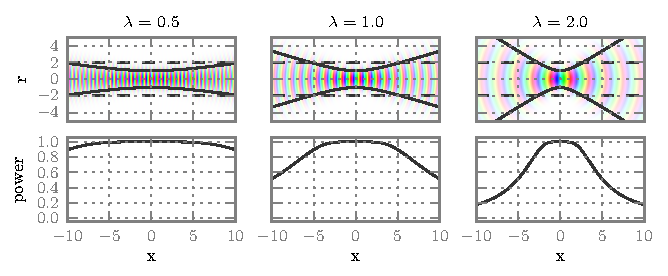
\includegraphics[width=\textwidth]{self_diffraction}
    \caption{
        These plots illustrate the effect of the self-diffraction of a Gaussian beam
        on the power detected by an apperture.
        Three Gaussian beams of different wavelengths
        are propagating along the $\vectu{x}$ axis.
        Their waist is placed at $x=0$.
        \emph{Top}:
            Amplitude $E(r, x)$ (color saturation) and
            phase (color hue) of the electric field of the beam,
            as a function of~$x$ and the distance~$r$ to the axis.
            The black solid lines show the beam width, defined by $E(r,x)=E(0,x) / e$
            where~$e$ is the base of the natural logarithm.
            Distances and wavelengths are normalized to the beam width at the waist.
            The dashed lines show the radius of a detector.
        \emph{Bottom}:
            Power (normalized to 1) flowing through a plane circular apperture of radius~2
            (between the dotted lines on top-row plots),
            placed on the beam axis, perpendicular to the beam axis, as a function of~$x$.
    }
    \label{fig:self-diffraction}
\end{figure}

In the particular case of HIFI, a model based on plane waves should provide a good approximation.
First, most of the optical elements of HIFI are placed at the waist of the beams, where the wavefront is plane.
Second, HIFI has well-designed and matched optics, so that the dominant reflections in the system always reflect power back in roughly the same beam mode.
Third, HIFI makes use of corrugated horns to couple the optical beams to the local oscillator diodes or the mixers.
When corrugated horns are used with properly tuned waveguides, they emit and receive single-mode beams \parencite{clarricoats1966propagation}.
Similarly, a device designer makes sure that his microwave circuit optimally couples to the fundamental waveguide mode by making a selection of coupling structures, device substrates, and in general by assuring an impedance match to the electromagnetic environment.
In other words, if any energy is converted to a high-order mode by the optics, then it does not couple to the mixer.
In that case, it is formally correct to model it with a simple term of loss.

In order to keep this chapter focused solely on interferences, some more general content has been gathered into~\cref{sec:complex_harmonic_plane_waves}, \nameref{sec:complex_harmonic_plane_waves}.
In this appendix, we derive the laws of refraction and reflection for complex harmonic plane waves: plane waves with complex fields, complex wave vectors and complex frequencies.
This work was motivated by the desire to treat metals and dielectrics on an equal footing.
It allows a proper treatment of materials that are lossy without being perfect conductors, for any angle of incidence.
In this general case, the iso-phase and iso-amplitude planes of a wave do not coincide.
By allowing the wave vector (not simply the wave number) to be complex, we decouple the direction of propagation from the direction of decay.
By using complex frequencies, we allow my model to compute the response of a time-invariant system to a time-varying input\footnote{
Infinitely differentiable only: a Laplace Transform could model infinite slopes (ideal switch on/off), but these are usually unphysical.
} without having to step through time.
The result is a much more general, elegant and useful expression of Snell's law and Fresnel's equations for plane waves in passive linear isotropic homogeneous materials.
In the current chapter, we apply the results of~\cref{sec:complex_harmonic_plane_waves} to the interferences in cavities.

We will begin this chapter with the study of a simple cavity.
This will provide a concrete example to illustrate the more abstract second part of this chapter, in which we detail the mathematics of our model.
Next, we will describe a complete implementation of our model with algorithms that can easily be translated into any imperative programming language.
Finally, we will provide a short catalog of typical optical elements that can be used with our model.





%#############################################################################
\FloatBarrier


\section{Gain modulation}
\label{sec:from_cavity_to_ripple}
\label{sec:fabry_perot_example}

Cavities can have a dramatic effect on the gain of a coherent receiver, as illustrated in~\cref{fig:mars_50010cb7_WBSH_USB_chp2}.
The baseline of this spectrum present a strong ripple with a period of~\SI{90}{\mega\hertz}.
Atmospheric models of Mars predict that the baseline of this spectrum, on each side of the absorption line, should be featureless.
This indicates that the ripple is an instrumental artifact: interferences in cavities modulate the gain of the instrument.
In this section, we will show how cavities produce ripples.
\begin{figure}
    \centering
    \includegraphics[width=\textwidth]{mars_50010cb7_WBSH_USB}
    \caption{Interferences have modulated the baseline of this HIFI spectrum of the planet Mars.
        Source: Herschel Science Archive, obsid 0x50010cb7.
    }
    \label{fig:mars_50010cb7_WBSH_USB_chp2}
    % obsid 0x50010cb7, 2012-05-24, OD 1106
    % AOT single point
    % Proposal      "KPGT_pharto01_1"
    % Proposal name "Mars CO 5-4 window 5"
    % Observer      "pharto01"
    % HifiPointModeDBS
    % raNominal  163.09653265005198 deg
    % decNominal 8.449952059887298  deg
    % radec system ICRS 2000
    % frame: heliocentric
    % redshift type: redshift
    % redshift frame: LSR
    % vlsr 0  (redshift value in km/s if redshiftType is optical or radio)
    % Band 1b
    % LO frequency measured 570.44025      # Actually tuned
    % LO frequency          570.4664221..  # modified for redshift
    % LOFcode               [97769, 68063] => 570.44025
    % forward eff 0.96
\end{figure}

An optical cavity is an arrangement of two or more reflective (or semi-reflective) surfaces that reflect the light waves back and forth between them.
The light interferes with itself constructively or destructively according to its frequency, the length of the cavity and the properties of the propagation medium.

One of the simplest types of cavity is the Fabry-Pérot\index{Fabry-Pérot} etalon, which is typically made of a single transparent plate with plane and parallel surfaces.
We can find these in heterodyne instruments, where they can be used as beam splitters (either directly, or as substrate to a wire grid polarizer).

In this section, we derive the reflection and transmission coefficients and gains of a Fabry-Pérot etalon for a homogeneous plane wave at normal incidence.
This will show how a cavity in the optical path of a coherent instrument can produce ripples on the baseline of a spectrum.



%=============================================================================

\subsection{Reflection and transmission coefficients of a cavity}

We consider three linear homogeneous and isotropic propagation media $A$, $B$ and $C$
delimited by two plane and parallel interfaces, as illustrated in~\cref{fig:cavity_notations}.
In~\cref{sec:complex_harmonic_plane_waves}, we have shown how the interface between two propagation media partially reflects and transmits electromagnetic waves.
These two interfaces, separated by a distance $L$, form a cavity.

Let us consider the general case in which the reflection and transmission coefficients differ for each side of each interface,
which happens in practice when the three media have different electric permittivities and magnetic permeabilities.

Each interface has two sides, so we have four sides in total that we label with the numbers~1 to~4,
four coefficients of reflection~$\cp{r}_1$ to~$\cp{r}_4$ and
four coefficients of transmission~$\cp{t}_1$ to~$\cp{t}_4$.

We represent the amplitude, phase and direction of the electric fields of the plane waves on each side of the interface with phasors.
We introduced phasors in~\cref{sec:phasor_notation}.

We assume that all the waves are plane, harmonic and homogeneous
(see~\cref{sec:complex_harmonic_plane_waves})
and that the wave vectors are normal to the interfaces.
As a result, all the electric fields in this problem are collinear.
This makes our problem one-dimensional.
We can therefore use scalar phasors instead of vector phasors.
This shortens our demonstration without diminishing its value.

We use the letter~$\cp{a}$ to indicate the phasor of a wave propagating toward an interface and the letter~$\cp{b}$ when the wave propagates away from an interface.

We call $\cp{a}_1$ the incident electric field phasor at the position of the $AB$ interface,
this represents the plane wave emitted by the source, the only input to the system.

We are interested in the outputs $\cp{b}_1$ and $\cp{b}_4$.
The plane wave of phasor~$\cp{b}_4$ at the interface $BC$ propagates towards a detector (not represented): it is the wave that our instrument detects.
The plane wave of phasor~$\cp{b}_1$ at the interface $AB$ propagates back to the source.

Finally, we call $\cp{d}$ the coefficient of propagation for the distance~$L$ in the medium~$B$.

\begin{figure}
    \centering
    \input{cavity.pdf_tex}
    \caption{Fabry-Pérot etalon, notations.}
    \caption*{
       The vertical dotted lines represent the interfaces between the propagation media $A$, $B$ and~$C$.
       The solid arrows represent coefficients of reflection, transmission and propagation.
       $\cp{r}$ is a coefficient of reflection.
       $\cp{t}$ is a coefficient of transmission.
       The dotted arrows represent the direction of propagation of plane waves.
       $\cp{a}$ is the electric phasor of a wave propagating toward an interface and
       $\cp{b}$ that of a wave propagating away from an interface.
       $\cp{d}$ is the coefficient of propagation for the distance~$L$ in the medium~$B$.
    }
    \label{fig:cavity_notations}
\end{figure}

All these quantities are linked by the following equations.
\begin{subequations}
    \begin{align}
    \cp{a}_2 &= \cp{d} \cp{b}_3                       \label{eq:cavity_rel_a2} \\
    \cp{a}_3 &= \cp{d} \cp{b}_2                       \label{eq:cavity_rel_a3} \\
    \cp{b}_1 &= \cp{t}_2 \cp{a}_2 + \cp{r}_1 \cp{a}_1 \label{eq:cavity_rel_b1} \\
    \cp{b}_2 &= \cp{t}_1 \cp{a}_1 + \cp{r}_2 \cp{a}_2 \label{eq:cavity_rel_b2} \\
    \cp{b}_3 &= \cp{r}_3 \cp{a}_3                     \label{eq:cavity_rel_b3} \\
    \cp{b}_4 &= \cp{t}_3 \cp{a}_3                     \label{eq:cavity_rel_b4}
    \end{align}
\end{subequations}
By substitution, we can compute the value of~$\cp{a}_3$ which is required to find~$\cp{b}_4$.
\begin{align}
    \cp{a}_3
    &= \cp{d} \cp{b}_2                                                 \notag \\
    &= \cp{d} \cp{t}_1 \cp{a}_1 + \cp{d}   \cp{r}_2 \cp{a}_2           \notag \\
    &= \cp{d} \cp{t}_1 \cp{a}_1 + \cp{d}^2 \cp{r}_2 \cp{b}_3           \notag \\
    &= \cp{d} \cp{t}_1 \cp{a}_1 + \cp{d}^2 \cp{r}_2 \cp{r}_3 \cp{a}_3  \notag
    \\
    \cp{a}_3 \left(1 - \cp{d}^2 \cp{r}_2 \cp{r}_3 \right)
    &=
    \cp{d} \cp{t}_1 \cp{a}_1
    \notag
    \\
    \cp{a}_3
    &=
    \cp{d} \cp{t}_1 \frac{1}{\cp{1} - \cp{d}^2 \cp{r}_2 \cp{r}_3} \cp{a}_1
    \notag
    \\
    \cp{b}_4
    &=
    \cp{d} \cp{t}_1 \frac{1}{1 - \cp{d}^2 \cp{r}_2 \cp{r}_3} \cp{t}_3 \cp{a}_1
    \label{eq:cavity_b4_a1}
\end{align}
Likewise, we can compute~$\cp{a}_2$ in order to find~$\cp{b}_1$.
\begin{align}
    \cp{a}_2
    &=
    \cp{d} \cp{b}_3                                     
    \notag
    \\
    &=
    \cp{d} \cp{r}_3 \cp{a}_3
    \notag
    \\
    &=
    \cp{d}^2 \cp{r}_3 \cp{t}_1 \frac{1}{1 - \cp{d}^2 \cp{r}_2 \cp{r}_3} \cp{a}_1
    \notag
    \\
    \cp{b}_1
    &=
    \left(
        \cp{d}^2 \cp{r}_3 \cp{t}_1
        \frac{1}{1 - \cp{d}^2 \cp{r}_2 \cp{r}_3} \cp{t}_2 + \cp{r}_1
    \right)
    \cp{a}_1
    \label{eq:cavity_b1_a1}
\end{align}
Equations~\eqref{eq:cavity_b4_a1} and \eqref{eq:cavity_b1_a1} give us the outputs of our cavity for an input~$\cp{a}_1$.
The reflection and transmission coefficients $\cp{r}$ and $\cp{t}$ of our cavity are
\begin{subequations}
\begin{align}
    \cp{r} &\equaldef
    \frac{\cp{b}_1}{\cp{a}_1}
    =
    \cp{r}_1 + \cp{d}^2 \cp{r}_3 \cp{t}_1 \cp{t}_2
    \frac{1}{1 - \cp{d}^2 \cp{r}_2 \cp{r}_3}
    \label{eq:cavity_reflection_coefficient}
    \\
    \cp{t} &\equaldef
    \frac{\cp{b}_4}{\cp{a}_1}
    =
    \cp{d} \cp{t}_1 \cp{t}_3
    \frac{1}{1 - \cp{d}^2 \cp{r}_2 \cp{r}_3}
    \text{.}
    \label{eq:cavity_transmission_coefficient}
\end{align}
\end{subequations}

\begin{samepage}
Both equations have a term in $\frac{1}{1 - \cp{d}^2 \cp{r}_2 \cp{r}_3}$.
This fraction has the shape of $\frac{1}{1 - \cp{q}}$
with $\cp{q}=\cp{d}^2 \cp{r}_2 \cp{r}_3$.
The quantity $\frac{1}{1 - \cp{q}}$ is the limit of the sum of the infinite series
\begin{equation}
    1 + \cp{q} + \cp{q}^2 + \cp{q}^3 + \ldots
    =
    \sum_{j=0}^\infty \cp{q}^j
    =
    \frac{1}{1-\cp{q}}
    \label{eq:infinite_series}
\end{equation}
as long as $\abs{\cp{q}} < 1$.
In our case $\cp{q}=\cp{d}^2 \cp{r}_2 \cp{r}_3$ represents the effect on the phase and the amplitude of a complete round-trip inside the cavity: $\cp{r}_2$ and $\cp{r}_3$ model the reflections on both interfaces and $\cp{d}^2$ models crossing the space between these interfaces twice.
The term $\frac{1}{1 - \cp{d}^2 \cp{r}_2 \cp{r}_3}$ models the effect of an infinite amount of round-trips of the electromagnetic wave inside the cavity.
\end{samepage}




%=============================================================================

\subsection{Reflection and transmission gain of a cavity}

We define the reflection gain~$R$ and the transmission gains~$T$ of the cavity with
\begin{align}
    R &\equaldef \frac{\power{P}_{b_1}}{\power{P}_{a_1}} \\
    T &\equaldef \frac{\power{P}_{b_4}}{\power{P}_{a_1}}
\end{align}
in which $\power{P}_{a_1}$, $\power{P}_{b_1}$ and $\power{P}_{b_4}$ are the active power carried by the waves of phasor $\cp{a}_1$, $\cp{b}_1$ and $\cp{b}_4$.

In~\cref{sec:time_averaged_complex_poynting_vector} we derived the expression of the time-averaged active Poynting vector of a homogeneous plane wave in a linear uniform isotropic medium,
\cref{eq:complex_poynting_homogeneous_real},
which we reproduce here:
\begin{align}
    \Re\left( \Timeavg{\vectcp{\power{S}}} \right)
    &=
    \frac{1}{2}
    \exp(2\omega_\im t)
    Y_\re % \Re\left(\sqrt{\frac{\cp{\epsilon}}{\cp{\mu}}}\right)
    \norm{\vect{e}_1}^2
    \vectu{k}
    %
    &
    %
    \text{with }
    Y_\re = \Re\left( \sqrt{\frac{\cp{\epsilon}}{\cp{\mu}}} \right)    
    \text{.}
    \tag{\ref{eq:complex_poynting_homogeneous_real}}
\end{align}
In this equation,
$\omega_\im$ is the imaginary part of the angular frequency,
$t$ is the time coordinate,
$Y_\re$ is the real part of the admittance (also called conductance),
$\cp{\epsilon}$ the electric permittivity,
$\cp{\mu}$ the magnetic permeability,
$\vectcp{e}_1$ the phasor of the electric field at the location of interest, and
$\vectu{k}$ the unit vector pointing in the direction of the wave vector.

This time-averaged active Poynting vector $\timeavg{\vect{\mathcal{P}}}$ is a directional irradiance, in watt per square meter.
We want the scalar power~$\power{P}_\Sigma$ flowing through an aperture $\Sigma$.
Both quantities are linked by
\begin{equation}
    \power{P}_\Sigma
    =
    \iint_\Sigma
    \!
    \Timeavg{\vect{\mathcal{P}}}
    \cdot
    \vectu{n}_\sigma
    \,
    \dif\sigma
    \tag{\ref{eq:active_reactive_power_from_poynting_vector}}
\end{equation}
where $\vectu{n}_\sigma$ is the unit vector normal to the surface element~$\dif\sigma$.

\begin{samepage}
We define two surfaces:
\begin{itemize}
    \item 
        $\Sigma_s$, of area $\mathcal{A}_{\Sigma_s}$,
        is the aperture by which the power emitted by the source enters the system
        and the power reflected by the cavity exits the system.
    \item
        $\Sigma_m$, of area $\mathcal{A}_{\Sigma_m}$,
        is the surface of the mixer (our detector) receiving the power transmitted by the cavity.
\end{itemize}
\end{samepage}
Both surfaces are plane and normal to the direction of propagation,
which implies that $\vectu{k}\cdot\vectu{n}_\sigma=\pm1$.
It also implies that $\timeavg{\vect{\power{P}}}$ is uniform on the surfaces and be factored out of the integrals, which reduce to the areas:
\begin{equation}
    \power{P}_\Sigma
    =
    \timeavg{\vect{\power{P}}}
    % start integral
    \iint_\Sigma
    \!
    %\vectu{k}
    %\cdot
    %\vectu{n}_\sigma
    %\,
    \dif\sigma
    % end integral
    =
    \frac{1}{2}
    \exp(2\omega_i t)
    Y_r
    \norm{\vect{e}_1}^2
    \mathcal{A}_\Sigma
    \text{.}
\end{equation}
We also need a factor~$\eta$ to account for the alignment of our two surfaces;
$\eta=1$ means that the surfaces are optimally aligned, maximizing power transfer,
while $\eta=0$ means that the mixer does not see any power from the source.
We assume that the power that does not couple to the mixer (case $\eta<1$) is lost: the wave impedes on the arbitrary surface located behind the mixer and is scattered/absorbed randomly.
The expressions of the input and output powers
$\power{P}_{a_1}$, $\power{P}_{b_1}$ and $\power{P}_{b_4}$ are
\begin{align}
    \power{P}_{a_1}
    &=
    \phantom{\mathrel{-}}
    \frac{1}{2}
    \exp(2\omega_i t)
    Y_{Ar}
    \norm{\vectcp{a}_1}^2
    \mathcal{A}_{\Sigma_s}
    \\%-------------
    \power{P}_{b_1}
    &=
    -
    \frac{1}{2}
    \exp(2\omega_i t)
    Y_{Ar}
    \norm{\vectcp{b}_1}^2
    \mathcal{A}_{\Sigma_s}
    \\%-------------
    \power{P}_{b_4}
    &=
    \phantom{\mathrel{-}}
    \frac{1}{2}
    \exp(2\omega_i t)
    Y_{Cr}
    \norm{\vectcp{b}_4}^2
    \mathcal{A}_{\Sigma_m}
    \eta
\end{align}
Since $\norm{\vectcp{b}_1}^2 = \abs{\cp{r}}^2 \norm{\vectcp{a}_1}^2$
and   $\norm{\vectcp{b}_4}^2 = \abs{\cp{t}}^2 \norm{\vectcp{a}_1}^2$,
the gains~$R$ and~$T$ are
\begin{align}
    R
    &=
    -\abs{\cp{r}}^2
    \label{eq:fabry_gain_r}
    \\%-------------------
    T
    &=
    \eta
    \frac{\mathcal{A}_{\Sigma_m}}{\mathcal{A}_{\Sigma_s}}
    \frac{Y_{Cr}}{Y_{Ar}}
    \abs{\cp{t}}^2
    \text{.}
    \label{eq:fabry_gain_t}
\end{align}
The minus sign in the expression of the reflection gain comes from the direction of the power flow through the aperture~$\Sigma_s$: positive when the power enters the system, negative when it leaves.
The minus sign can be ignored when the direction does not matter.





%=============================================================================

\subsection{Periodicity of the gains}
\label{sec:periodicity_in_power}

For the cavity to create ripples on a spectrum (see \vref{fig:mars_50010cb7_WBSH_USB_chp2}), $T$ must be a periodic (or at least oscillating) function of the frequency.
Assuming that the materials $A$, $B$ and $C$ are not dispersive, the only source of periodicity is the propagation coefficient $\cp{d}$, which models the effect on the phase and amplitude of propagating inside the cavity.


%-----------------------------------------------------------------------------

\subsubsection{Periodicity of the propagation coefficient}

If $L$ is the distance between the two interfaces, then the value of $\cp{d}$ is given by
\begin{equation}
    \cp{d} = \exp \left( i\cp{k}_B L \right) \label{eq:cavity_s_k}
\end{equation}
where $\cp{k}_B$ is the wave number in the medium~$B$.
The wavenumber~$\cp{k}_B$ and the angular frequency~$\cp{\omega}$ are related by
\begin{equation}
    \cp{k}_B
    =
    \frac{\cp{\omega}}{\cp{c}_B}
    =
    \cp{\omega} \sqrt{\cp{\epsilon}_B \cp{\mu}_B}
\end{equation}
with $\cp{c}_B$, $\cp{\epsilon}_B$ and $\cp{\mu}_B$ the phase velocity, electric permittivity and magnetic permeability of the medium~$B$.

To shorten the equations, we remove the subscript $B$ from all quantities; the medium~$B$ is assumed by default.
Furthermore, we call~$\cp{\alpha}=\sqrt{\cp{\epsilon} \cp{\mu}}$.
We inject this expression of~$\cp{k}$ in that of~$\cp{d}$, then we separate the real and imaginary parts of the argument of~$\cp{d}$ to reveal its periodicity as a function of the real angular frequency~$\omega_r = \Re(\cp{\omega})$.
\begin{subequations}
    \label{eq:distance_coefficient_expanded}
    \begin{align}
        \cp{d}
        &=
        \exp \left( i \cp{\omega} \cp{\alpha} L \right)
        \\
        &=
        \exp
        \left[
            i
            (\omega_r + i \omega_i) (\alpha_r + i \alpha_i)
            L
        \right]
        \\
        &=
        \exp
        \left[
            -
            (\omega_r \alpha_i + \omega_i \alpha_r)
            L
        \right]
        \;
        \exp
        \left(
            -i \omega_i \alpha_i L
        \right)
        \;
        \exp
        \left(
            i \omega_r \alpha_r L
        \right)
    \end{align}
\end{subequations}
The third exponential is complex and involves the real angular frequency~$\omega_r$;
this makes $\cp{d}$ a periodic function of the real frequency~$f_r=\omega_r/(2\pi)$.
The period is
\begin{equation}
    F_d = 
    \frac{1}{\Re(\sqrt{\cp{\epsilon}\cp{\mu}})L}
    \text{.}
\end{equation}

To be rigorous, $\cp{d}$ is periodic only if $\alpha_i=0$, which is required to cancel the contribution of $\omega_r$ to the first exponential.
If the medium $B$ is dielectric, $\epsilon_i=0$ and $\mu_i=0$, which implies that $\alpha_i=0$.
If metals are involved, then $\cp{d}$ may be oscillating%
\footnote{
Periodic function: $f$ is periodic if $\exists T, T \ne 0, \forall t, f(t)=f(t+T)$.  The smallest positive value of $T$ satisfying this condition is called the period of $f$.\\
Almost-periodic function: the function is periodic within a defined level of accuracy, its regularity increases over multiple periods.  Example: planetary orbits.\\
Quasiperiodic function: the periodicity of $f$ is irregular and unpredictable.  Example: El Ni\~no (`period' varies between 4 and 12 years, spectral density peaks at 5 years).\\
Pseudo-periodic function: function of several variables that has a period for each variable.\\
Oscillating function: the function moves between extremes.  Examples: $x \mapsto \sin(1/x)$ or $x \mapsto \sin(x)/x$.
}
rather than periodic: the period itself may be a function of frequency and can therefore be defined only locally.



%-----------------------------------------------------------------------------

\subsubsection{Effect on the gains}
\label{sec:fabry_gain}

According to~\cref{eq:fabry_gain_r,eq:fabry_gain_t},
the periodicity of the reflection and transmission gains is that of~$\abs{\cp{r}}^2$ or $\abs{\cp{t}}^2$.
\begin{equation}
    \abs{\cp{t}}^2 = \abs{\cp{d}}^2 \abs{\cp{t}_1}^2 \abs{\cp{t}_3}^2
    \abs{
        \frac{1}{1 + \cp{d}^2 \cp{r}_2 \cp{r}_3}
    }^2
    \label{eq:fabry_gain_r2_r3}
\end{equation}
In this equation, $\cp{d}$ is periodic but its modulus is not,
so the periodicity of~$\abs{\cp{t}}^2$ comes from the fraction.
We can say the same for the reflection.
The fraction is the sum of an infinite series (see~\cref{eq:infinite_series}); we can expand it at the first order:
\begin{equation}
    \abs{
        \frac{1}{1 + \cp{d}^2 \cp{r}_2 \cp{r}_3}
    }^2
    =
    \abs{
        1 + \cp{d}^2 \cp{r}_2 \cp{r}_3 + \ldots
    }^2
\end{equation}
We pose
$\cp{d} = \cp{d}' \exp(i\phi_d)$ with $\phi_d = \omega_r/F_d$.
We also pose
$\cp{q} = \cp{d}^2 \cp{r}_2 \cp{r}_3$ and write it in polar form:
\begin{align}
    \cp{q}
    &=
    \cp{d}'^2 \exp(i2\phi_d)    \;
    r_2 \exp(i\phi_{r_2}) \;
    r_3 \exp(i\phi_{r_3})
    \\
    &=
    \underbrace{\cp{d}'^2 r_2 r_3}_{=\cp{q}'}
    \exp
    \Big(
        i
        \underbrace{(2 \phi_d + \phi_{r_2} + \phi_{r_3})}_{=\phi_q}
    \Big)
\end{align}
Now we can compute $\abs{1+\cp{q}}^2$:
\begin{align}
    \abs{1+\cp{q}}^2
    &=
    (1+\cp{q}) (1+\cp{q})^*
    \\
    &=
    \Big(1 + \cp{q}' \exp(i\phi_q)\Big)
    \Big(1 + \cp{q}' \exp(-i\phi_q)\Big)
    \\
    &=
    1 + \cp{q}'^2 + \cp{q}' \big( \exp(i\phi_q) + \exp(-i\phi_q) \Big)
    \\
    &=
    1 + \cp{q}'^2 + 2\cp{q}' \cos(\phi_q)
    \\
    &=
    1 + \cp{q}'^2 + 2\cp{q}' \cos(2 \phi_d + \phi_{r_2} + \phi_{r_3})
\end{align}
Since~$\phi_d = \omega_r/F_d$, $\abs{1+\cp{q}}^2$ has for period~$F=F_d/2$.
This is the fundamental period of $\abs{\cp{r}}^2$ and $\abs{\cp{t}}^2$.
If we expand the fraction to higher orders
we get harmonics of periods $F/2$, $F/3$, $F/4$, etc.
When the cavity is lossy (absorption in the propagation medium and/or low reflection on the surfaces) then $\abs{\cp{q}}$ is low and the amplitudes of the harmonics decrease rapidly: a single sine is a good approximation of a lossy cavity.
These periodicities transfer to the reflection and transmission gains of the system, $R$ and $T$.

To summarize:
The cavity modulates the reflection and transmission gains of the system.
This modulation is periodic (or oscillating).
The fundamental period of this modulation is
\begin{equation}
    F = 
    \frac{1}{2\Re(\sqrt{\cp{\epsilon}\cp{\mu}})L}
    \text{.}
    \label{eq:relation_length_period_nice}
\end{equation}
This periodic modulation of the transmission gain of the system is responsible for the ripples observed on the baseline of the spectrum shown in~\cref{fig:mars_50010cb7_WBSH_USB_chp2}.

In a more realistic system, the materials are dispersive (their electric permittivity and magnetic permeability depend on the frequency), and the reflection and transmission gains may not be really periodic, but only oscillating.



%-----------------------------------------------------------------------------

\subsubsection{Energy conservation}

When the interferences are destructive on the detector-side of the cavity, they are constructive on the source-side: the power is sent back to the source%
\footnote{
    This actually could cause the source to be influenced,
    for example if a laser (that is a cavity in itself) is coupled to an external cavity,
    the effective frequency of the laser could be changed.
}.
This is illustrated by~\cref{fig:cavity_energy_conservation}.
\begin{figure}
    \centering
    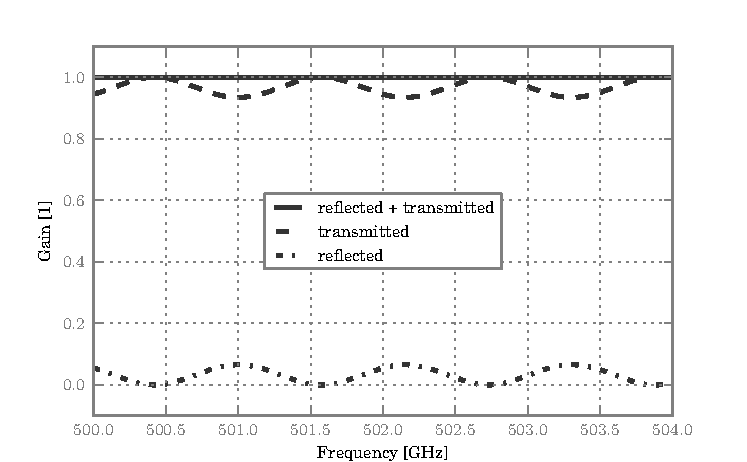
\includegraphics{cavity_energy_conservation}
    \caption{Power conservation in a lossless cavity.}
    \caption*{
        The power that enters a cavity can either be transmitted through the cavity, reflected by it, or anything in-between.
    }
    \label{fig:cavity_energy_conservation}
\end{figure}
In order to create~\cref{fig:cavity_energy_conservation}, we had to use physically-plausible values for the reflection and transmission coefficients of the cavity.
The reflection and transmissions coefficients were derived using lossless media, Fresnel's equations for normal incidence (see~\vref{sec:fresnel_normal_incidence})
and assuming that the aperture and mixer surfaces were identical and aligned.

In a sense, a lossless cavity is a filter that can be either totally transmissive, totally reflective, or anything in-between, depending on the frequency of the wave.

What we have just done for a single cavity in one dimension can be done for an arbitrarily large amount of interconnected cavities in three dimensions.
This is what we are going to show in the next section, in which we describe the mathematics with which we represent optical elements and their connections.



%#############################################################################
\FloatBarrier
\section{Mathematics of the model}
\label{sec:chapter2_3}

In this section, we present the method that we developed to compute the gain of a coherent optical system.
Our method is unique in that it solves directly for the steady state of the electromagnetic fields and takes into account the interferences caused by the reflections between every pair of surfaces along every possible optical paths.
To do that, we model the optical system with a set of linear equations and solve it.

At its core, our method relies on an abstraction of an optical system that we call ``network''.
A network can represent either a concrete optical element such as a mirror, or an arbitrarily complex configuration of interconnected elements such as the entire focal plane unit of HIFI described by~\textcite{jackson2002hifi}.

In electrical engineering, the term ``network'' refers to an interconnection of discrete electrical components, potentially degenerated to a single component.
Transmission-line theory extends the meaning of ``network'' to include non-discrete elements such as an arbitrary length of cable.
Applying the notion of networks to optics is not a new idea,
it can be found in~\textcite{siegman1986lasers},
but it is a powerful one.

Networks have one or more ``ports'' that allow them to be connected to other networks.
When two ports are connected, the output of each port is the input of the other.
For example, \cref{fig:fp_networks} represents the Fabry-Pérot etalon that we studied in the previous section: the rectangles represent networks, the dots represent ports, and the lines represent connections between ports.
The whole Fabry-Pérot elaton can be seen either as a single two-port network or as three connected elementary two-port networks.
\begin{figure}
    \centering
    \input{fp_networks.pdf_tex}
    \caption{Constitutive networks of a Fabry-Pérot etalon.}
    \label{fig:fp_networks}
\end{figure}

Each port has one input and one output.
The $n$ inputs and $n$ outputs of a $n$-port network are related by a set of equations.
For our study, we assume that these equations are linear,
which allows us to represent a $n$-port network with a $n$--by--$n$ matrix.

Circuit theory introduces several types of matrices that can model networks.
The chapter~4 of \textcite{pozar2009microwave} describes matrices of impedance parameters, admittance parameters, hybrid parameters, ABCD parameters, etc., which all correspond to a different choice of input and output quantities for the networks, namely various combinations of electric voltages and currents.
Voltages and currents are not convenient when working at frequencies above a gigahertz, they become difficult to measure and somewhat abstract for waves propagating in free space;
at high frequencies, it is easier to measure the power of a wave, or its intensity (proportional to the square root of that power).
\textcite{pozar2009microwave} describes another set of parameters called ``scattering parameters'', which together form a ``scattering matrix'', that are more adapted to our situation.
Indeed, the scattering parameters convey the ideas of incident, reflected and transmitted wave intensity.
In our model, we model networks with scattering matrices.

The vocabulary may be confusing.
The word ``network'' commonly refers to several distinct entities and their relations.
In this chapter, the word ``network'' refers to anything that has a scattering matrix.


From a list of scattering matrices representing each network, and a description of how the ports of these networks are connected, our solver determines the reflection coefficient of each port, and the transmissions coefficients between each port and every other port.
We will now describe the mathematics that solve for these coefficients.





%=============================================================================

\subsection{Scattering matrices}

Scattering matrices \parencite{pozar2009microwave,siegman1986lasers} model the transfer of power or field intensity between the ports of a network.
In coherent systems, scattering matrices operate on the intensity and the phase of the electromagnetic waves, not their power.
Indeed, in coherent systems the electromagnetic fields add linearly but the powers do not: two fields of equal amplitude carry the same power, but if they have opposite phases, their sum carries no power at all.

\Cref{fig:scattering_matrix_notations} presents the notation that we will use in the rest of this chapter in the particular case of a 4-port network.
The ports of a network are numbered.
Following the conventional notations for scattering matrices,
the input to the port number $i$ is noted $\cp{a}_i$ and its output is noted~$\cp{b}_i$.
The inputs and outputs of a network are complex numbers.

\begin{figure}[b]
    \centering
    \input{scattering_matrix_notations.pdf_tex}
    \caption{A 4-port network showing four inputs $\cp{a}_i$ and four outputs $\cp{b}_i$.}%
    \caption*{For example, this network could be a wire grid polarizer or a semi-transparent mirror, both acting as beam splitters.}
    \label{fig:scattering_matrix_notations}
\end{figure}

The scattering parameters, that is the elements of a scattering matrix, which relate the inputs to the outputs, are also complex numbers.
The relation between a vector of inputs $\vectcp{a}$, a vector of outputs $\vectcp{b}$, and a scattering matrix~$\matrcp{S}$ is simply given by the matrix product
\begin{equation}
    \vectcp{b} = \matrcp{S} \vectcp{a}
\end{equation}
which, in the case of a $n$-port network, can be expanded into
\begin{equation}
    \begin{pmatrix}
        \cp{b}_1\\
        \cp{b}_2\\
        \vdots\\
        \cp{b}_n
    \end{pmatrix}
    =
    \begin{pmatrix}
        \cp{S}_{1, 1} & \cp{S}_{1, 2} & \cdots & \cp{S}_{1, n} \\
        \cp{S}_{2, 1} & \cp{S}_{2, 2} & \cdots & \cp{S}_{2, n} \\
        \vdots   & \vdots   & \ddots & \vdots   \\
        \cp{S}_{n, 1} & \cp{S}_{n, 2} & \cdots & \cp{S}_{n, n}
    \end{pmatrix}
    \begin{pmatrix}
        \cp{a}_1\\
        \cp{a}_2\\
        \vdots\\
        \cp{a}_n
    \end{pmatrix}
    \text{.}
    \label{eq:scattering_matrix}
\end{equation}

For a scattering matrix to accurately represent the reflections and transmissions of a network, the inputs and outputs must be matched to these ports.
Let us explain this with an example.
The Fabry-Pérot etalon that we studied in~\cref{sec:fabry_perot_example} can be represented with three networks, as we showed with~\cref{fig:fp_networks}.
Using the notations introduced in~\vref{fig:cavity_notations},
these three networks have the following scattering matrices:
\begin{align}
    \matrcp{S}_\text{interfaceAB}
    &=
    \begin{pmatrix}
        \cp{r}_1 & \cp{t}_2 \\
        \cp{t}_1 & \cp{r}_2
    \end{pmatrix}
    \\
    \matrcp{S}_\text{space}
    &=
    \begin{pmatrix}
        0      & \cp{d} \\
        \cp{d} & 0
    \end{pmatrix}
    \\
    \matrcp{S}_\text{interfaceBC}
    &=
    \begin{pmatrix}
        \cp{r}_3 & \cp{t}_4 \\
        \cp{t}_3 & \cp{r}_4
    \end{pmatrix}
    \text{.}
\end{align}
The parameters~$\cp{r}_4$ and $\cp{t}_4$ are not represented in~\cref{fig:cavity_notations}
because we did not consider, at the time, waves incident on the interface side number~4.
The scattering parameter $\matrcp{S}_\text{interfaceAB,1,1} = \cp{r}_1$ represents the coefficient of reflection of a wave incident to the interface side number~1 if there is nothing on that side of the interface but an infinite expanse of medium~$A$.
This is what is meant by matching the input to the network.
The scattering matrix of a network includes some assumptions about its environment;
it is defined for an ideal environment that matches its ports exactly.
In practice, when a network is connected to another, these two networks interact and the scattering parameters are not the actual reflection and transmission coefficients of the system.
Computing the actual reflection and transmission coefficients is the goal of our study.

We have not yet explained what, exactly, we use as inputs and outputs for the networks in our model.
This is the subject of the next section.




%=============================================================================

\subsection{Jones calculus in 3D}



%-----------------------------------------------------------------------------
\subsubsection{Jones calculus}

In order to model interferences in a coherent instrument, we must keep track at all time of the intensity, phase and polarization of the electromagnetic field.
\textcite{jones1941calculus} introduced a method for doing exactly that,
which was later named ``Jones calculus''.

Jones calculus introduces Jones vectors and Jones matrices.
A Jones vector encodes the intensity, phase and polarization of a plane wave.
A Jones matrix represents a linear transformation between Jones vectors, modeling the effect of an optical network on the intensity, phase and polarization of a wave.

Two Jones vectors $\vectcp{E}^a$ and~$\vectcp{E}^b$ and a Jones matrix~$\matrcp{J}$ are related by
\begin{equation}
    % Small form.
    \vectcp{E}^b = \matrcp{J} \vectcp{E}^a
    \label{eq:jones_matrix_short}
    \text{.}
\end{equation}

Although Jones calculus does not impose it, it is often convenient to define Jones vectors from the electric field of the wave, which is why we note them with the letter~$E$.
\Textcite{hecht2002optics} expands Jones vectors and Jones matrices in the following way:
\begin{equation}
    % Jones matrix in 2D.
    \begin{pmatrix}
        \cp{E}^b_h\\
        \cp{E}^b_v
    \end{pmatrix}
    =
    \begin{pmatrix}
        \cp{J}_{h, h}   &   \cp{J}_{h, v} \\
        \cp{J}_{v, h}   &   \cp{J}_{v, v}
    \end{pmatrix}
    \begin{pmatrix}
        \cp{E}^a_h\\
        \cp{E}^a_v
    \end{pmatrix}
    \label{eq:jones_matrix_2d}
\end{equation}
In that formalism,
a polarized electric field is seen as the superposition of a horizontal and a vertical component, both linearly polarized, noted $h$ and $v$.
The amplitude and phase difference between these components determines the handedness and the ellipticity of the polarization of the field.
If the horizontal and vertical components are in phase, then the field is linearly polarized; if their phase difference is~\SI{90}{\degree} then the field is circularly polarized.

\begin{samepage}
The linearity of the system allows us to use he same Jones matrix to relate the phasors of the two fields:
\begin{equation}
    \begin{pmatrix}
        \cp{e}^b_h\\
        \cp{e}^b_v
    \end{pmatrix}
    =
    \begin{pmatrix}
        \cp{J}_{h, h}   &   \cp{J}_{h, v} \\
        \cp{J}_{v, h}   &   \cp{J}_{v, v}
    \end{pmatrix}
    \begin{pmatrix}
        \cp{e}^a_h\\
        \cp{e}^a_v
    \end{pmatrix}
\end{equation}
in which~$\cp{e}^a_h$, $\cp{e}^a_v$, $\cp{e}^b_h$ and $\cp{e}^b_h$ are scalar phasors
representing~$\vectcp{E}^a$ and $\vectcp{E}^b$ in specific reference frames.
We described phasors in~\vref{sec:phasor_notation}.
\end{samepage}

\paragraph{Jones calculus and unpolarized waves.}
\label{sec:jones_unpolarized}
Jones calculus is unable to model networks that depolarize waves.
There exists another formalism called ``Mueller calculus'' named after Hans Mueller who developed it \parencite{mueller1943memorandum}.
Mueller calculus is a matrix method for manipulating Stokes vectors, which are four-dimensional real vectors that have room for unpolarized waves.
However, Mueller calculus works in power, not in field, which makes it unsuitable for modeling interferences, for which the phase of the field is needed.

Even though Jones calculus cannot model depolarizing networks, it can be applied to unpolarized waves.
\textcite{goodman1985statistical} explains in detail how an unpolarized or partially polarized wave can be represented in terms of polarized waves.
A totally unpolarized wave can be decomposed into two polarized waves of opposite polarizations and equal intensities.
These opposite polarizations are arbitrary; we can choose circular left and circular right, or more conveniently horizontal and vertical.
\begin{equation}
    \begin{aligned}
        \vectcp{E}^{ah}
        &=
        \frac{\cp{E}^a}{\sqrt{2}}
        \begin{pmatrix}
            1 \\ 0
        \end{pmatrix}
        \\
        \vectcp{E}^{av}
        &=
        \frac{\cp{E}^a}{\sqrt{2}}
        \begin{pmatrix}
            0 \\ 1
        \end{pmatrix}
    \end{aligned}
\end{equation}
Each polarization carries half of the surface power density of the wave.
What makes this wave unpolarized is that the phase difference between~$\vectcp{E}^{ah}$ and $\vectcp{E}^{av}$ varies randomly.
Independently, $\vectcp{E}^{ah}$ and $\vectcp{E}^{av}$ are coherent, but $\vectcp{E}^a$ is not.
Since $\vectcp{E}^{ah}$ and $\vectcp{E}^{av}$ are coherent, we can apply Jones calculus to them.
\begin{equation}
    \begin{aligned}
        \vectcp{E}^{bh}
        &=
        \matrcp{J}
        \vectcp{E}^{ah}
        \\
        \vectcp{E}^{bv}
        &=
        \matrcp{J}
        \vectcp{E}^{av}
    \end{aligned}
\end{equation}
We cannot add $\vectcp{E}^{bh}$ and $\vectcp{E}^{bv}$ in fields because their phases do not line up, but we can add them in power with
\begin{equation}
    P^b
    =
    \frac{1}{2}
    \left(
        Y^b_r \norm{\vectcp{E}^{bh}}^2 + Y^b_r \norm{\vectcp{E}^{bv}}^2
    \right)
\end{equation}
where $Y^b_r$ is the real part of the wave admittance of the wave $b$.
We explained power calculations in~\cref{sec:time_averaged_complex_poynting_vector}.

\paragraph{Jones calculus and independent sources.}
\label{sec:jones_independent}
The previous paragraph can be extended from unpolarized sources to completely independent sources.
Whenever two sources of electromagnetic waves that are not phase-locked to each other feed a system modeled with Jones matrices, the response of the system must be computed for each source independently and the results added in power.

For example, both the astronomical signal and the noise of the local oscillator enter the focal plane unit of HIFI at the same time but their phases are not correlated;
the two polarizations of the sky and the two polarizations of the local oscillator must be treated separately, yielding four output fields that we must add in power.



%-----------------------------------------------------------------------------

\subsubsection{Extension of Jones calculus to three dimensions}
Although very useful for many applications, the traditional Jones matrices and vectors have limitations.

First, the field is always expressed in a local reference frame: the horizontal and vertical directions are valid for one wave only and may change after a reflection or a refraction.
Therefore, to completely describe a field, the Jones vector is not enough and one needs to keep track of the orientation of its reference frame.

Second, the horizontal and vertical directions are normal to each other and to the direction of propagation.
This limits us to modeling either transverse electric or transverse magnetic waves depending on whether the Jones vector represents the electric or the magnetizing field%
\footnote{
The terminology varies in the literature.
In this chapter, we call~$\vectcp{E}$ and $\vectcp{B}$ ``electric'' and ``magnetic'' field intensities.
The electric and magnetic fields are the quantities figuring in Maxwell's microscopic equations.
The fields introduced in the macroscopic equations are~$\vectcp{D}$ and $\vectcp{H}$, which we call ``electric displacement'' and ``magnetizing'' field intensities.
See~\cref{sec:maxwell_macroscopic} for details.
};
this cannot model hybrid waves, in which both the electric and the magnetizing field can have a component along the direction of propagation.
Therefore, this cannot model propagation in birefringent materials~\footnote{We have not modeled birefringent material during our study; doing so would require reworking the derivations of~\cref{sec:complex_harmonic_plane_waves} to account for anisotropic propagation media.}.

To free ourselves from these limitations we express all the fields in a common global Cartesian reference frame, essentially extending Jones calculus from two to three dimensions:
\begin{equation}
    % Jones matrix in 3D.
    \begin{pmatrix}
        \cp{E}^b_x\\
        \cp{E}^b_y\\
        \cp{E}^b_z
    \end{pmatrix}
    =
    \begin{pmatrix}
        \cp{J}_{x, x}   &   \cp{J}_{x, y}   &   \cp{J}_{x, z} \\
        \cp{J}_{y, x}   &   \cp{J}_{y, y}   &   \cp{J}_{y, z} \\
        \cp{J}_{z, x}   &   \cp{J}_{z, y}   &   \cp{J}_{z, z}
    \end{pmatrix}
    \begin{pmatrix}
        \cp{E}^b_x\\
        \cp{E}^b_y\\
        \cp{E}^b_z
    \end{pmatrix}
    \text{.}
    \label{eq:jones_matrix_3d}
\end{equation}

\begin{samepage}
In phasor notation, this reduces to
\begin{equation}
    \vectcp{e}^b = \matrcp{J} \vectcp{e}^a
    \text{.}
\end{equation}
in which~$\vectcp{e^a}$ and $\vectcp{e}^b$ are vector phasors of the type we used in all of~\cref{sec:phasor_notation}.
\end{samepage}

When extended to three dimensions, Jones calculus deals not only with the amplitude and the phase of a wave, but also its direction.
In that light, the reflection and transmission matrices for an interface that we derived in~\vref{sec:fresnel_matrix} are Jones matrices.



%-----------------------------------------------------------------------------
\subsubsection{Rotating Jones matrices}
\label{sec:rotating_jones_matrices}

Another advantage of three-dimensional Jones matrices is that they can be combined with rotation matrices in order to represent networks in any orientation in space.
If $\matr{R}$ is a 3--by--3 rotation matrix and $\matrcp{J}$ a Jones matrix of a system in a given orientation,
then the Jones matrix $\matrcp{J}'$ corresponding to that system rotated by $\matr{R}$ is
\begin{equation}
    \matrcp{J}' = \matr{R} \, \matrcp{J} \, \matr{R}^{-1}
    \text{.}
    \label{eq:jones_rotation_using_inverse}
\end{equation}
The multiplication by~$\matr{R}^{-1}$ brings the electric phasor in the reference frame of the system at rest so that we can apply~$\matrcp{J}$.
The resulting electric phasor, expressed in the rest frame, is then rotated by~$\matr{R}$, which brings it back to the global reference frame.

Note: rotations matrices are orthogonal matrices (the norm of their rows and columns equals~1), therefore $\matr{R}^{-1} = \matr{R}\transp$.

%\Cref{eq:jones_rotation_using_inverse} is mathematically correct, however it may not be the most practical to implement.
%Indeed, inverting matrices is an expensive and unstable operation for a computer to perform
%When we remember that the inverse of a rotation matrix is also its transpose,
%then we get \cref{eq:jones_rotation_using_transpose} which has the advantage of being computationally cheap and stable.
%\begin{equation}
%    J' = R J R\transp
%    \label{eq:jones_rotation_using_transpose}
%\end{equation}

%Rotating the identity matrix has an interesting property shown by~\eqref{eq:jones_rotation_identity}.
%\begin{equation}
%    I' = R I R^{-1}
%       = R R^{-1}
%       = I
%    \label{eq:jones_rotation_identity}
%\end{equation}
%If a Jones matrix is proportional to an identity matrix, then it is not modified by rotation.
%We will use that property to save some computation, for example when propagating through homogeneous isotropic materials (\vref{sec:generic_networks_distance}).

%=============================================================================
\subsection{Combining scattering and Jones matrices}
Since Jones vectors describe polarized waves, we decided to model each input and output of a network with a Jones vector.
Each port of a network receives and emits a polarized wave.
This makes $\vectcp{a}$ and $\vectcp{b}$ vectors of Jones vectors.
As a consequence, each element of the scattering matrix $\matrcp{S}$ is a Jones matrix.
Using our notations for vectors (bold letters) and matrices (upright letters), \cref{eq:scattering_matrix} is rewritten
\begin{equation}
        \begin{pmatrix}
            \vectcp{b}_1\\
            \vectcp{b}_2\\
            \vdots\\
            \vectcp{b}_n
        \end{pmatrix}
    =
        \begin{pmatrix}
            \matrcp{S}_{1, 1} & \matrcp{S}_{1, 2} & \cdots & \matrcp{S}_{1, n} \\
            \matrcp{S}_{2, 1} & \matrcp{S}_{2, 2} & \cdots & \matrcp{S}_{2, n} \\
            \vdots   & \vdots   & \ddots & \vdots   \\
            \matrcp{S}_{n, 1} & \matrcp{S}_{n, 2} & \cdots & \matrcp{S}_{n, n}
        \end{pmatrix}
        \begin{pmatrix}
            \vectcp{a}_1\\
            \vectcp{a}_2\\
            \vdots\\
            \vectcp{a}_n
        \end{pmatrix}
    \text{.}
\end{equation}
Its expansion for a two-port network is
\begin{equation}
    \begin{gathered}
    \vectcp{b} = \matrcp{S} \vectcp{a}
    \\
    \begin{pmatrix}
        \vectcp{b}_1 \\ \vectcp{b}_2
    \end{pmatrix}
    =
    \matrcp{S}
    \begin{pmatrix}
        \vectcp{a}_1 \\ \vectcp{a}_2
    \end{pmatrix}
    \\
    \begin{pmatrix}
        \begin{pmatrix}
            \cp{b}_{1, x} \\ \cp{b}_{1, y} \\ \cp{b}_{1, z}
        \end{pmatrix}
        \\
        \begin{pmatrix}
            \cp{b}_{2, x} \\ \cp{b}_{2, y} \\ \cp{b}_{2, z}
        \end{pmatrix}
    \end{pmatrix}
    =
    \matrcp{S}
    \begin{pmatrix}
        \begin{pmatrix}
            \cp{a}_{1, x} \\ \cp{a}_{1, y} \\ \cp{a}_{1, z}
        \end{pmatrix}
        \\
        \begin{pmatrix}
            \cp{a}_{2, x} \\ \cp{a}_{2, y} \\ \cp{a}_{2, z}
        \end{pmatrix}
    \end{pmatrix}
    \\
    \matrcp{S} =
    \begin{pmatrix}
        \begin{pmatrix}
            \cp{S}_{1, 1, x, x} & \cp{S}_{1, 1, x, y} & \cp{S}_{1, 1, x, z} \\
            \cp{S}_{1, 1, y, x} & \cp{S}_{1, 1, y, y} & \cp{S}_{1, 1, y, z} \\
            \cp{S}_{1, 1, z, x} & \cp{S}_{1, 1, z, y} & \cp{S}_{1, 1, z, z} \\
        \end{pmatrix}
        &
        \begin{pmatrix}
            \cp{S}_{1, 2, x, x} & \cp{S}_{1, 2, x, y} & \cp{S}_{1, 2, x, z} \\
            \cp{S}_{1, 2, y, x} & \cp{S}_{1, 2, y, y} & \cp{S}_{1, 2, y, z} \\
            \cp{S}_{1, 2, z, x} & \cp{S}_{1, 2, z, y} & \cp{S}_{1, 2, z, z} \\
        \end{pmatrix}
        \\
        \begin{pmatrix}
            \cp{S}_{2, 1, x, x} & \cp{S}_{2, 1, x, y} & \cp{S}_{2, 1, x, z} \\
            \cp{S}_{2, 1, y, x} & \cp{S}_{2, 1, y, y} & \cp{S}_{2, 1, y, z} \\
            \cp{S}_{2, 1, z, x} & \cp{S}_{2, 1, z, y} & \cp{S}_{2, 1, z, z} \\
        \end{pmatrix}
        &
        \begin{pmatrix}
            \cp{S}_{2, 2, x, x} & \cp{S}_{2, 2, x, y} & \cp{S}_{2, 2, x, z} \\
            \cp{S}_{2, 2, y, x} & \cp{S}_{2, 2, y, y} & \cp{S}_{2, 2, y, z} \\
            \cp{S}_{2, 2, z, x} & \cp{S}_{2, 2, z, y} & \cp{S}_{2, 2, z, z} \\
        \end{pmatrix}
    \end{pmatrix}
    \text{.}
    \end{gathered}
    \label{eq:matrix_of_matrices}
\end{equation}

Matrices of matrices are compatible with simple algebraic operations (the product above follows the usual rule for multiplying matrices), but we prefer to interpret them as more conventional ``block matrices'' \parencite{eves2012elementary}.
They are conventional matrices, in the sense that they hold scalars, but they are subdivided in regions, or ``blocks''.
Mathematically, \cref{eq:matrix_of_matrices} is equivalent to
\begin{equation}
    \begin{pmatrix}
        \cp{b}_{1, x} \\ \cp{b}_{1, y} \\ \cp{b}_{1, z}
        \\
        \cp{b}_{2, x} \\ \cp{b}_{2, y} \\ \cp{b}_{2, z}
    \end{pmatrix}
    =
    \begin{pmatrix}
        \cp{S}_{1, 1, x, x} & \cp{S}_{1, 1, x, y} & \cp{S}_{1, 1, x, z}   &   \cp{S}_{1, 2, x, x} & \cp{S}_{1, 2, x, y} & \cp{S}_{1, 2, x, z} \\
        \cp{S}_{1, 1, y, x} & \cp{S}_{1, 1, y, y} & \cp{S}_{1, 1, y, z}   &   \cp{S}_{1, 2, y, x} & \cp{S}_{1, 2, y, y} & \cp{S}_{1, 2, y, z} \\
        \cp{S}_{1, 1, z, x} & \cp{S}_{1, 1, z, y} & \cp{S}_{1, 1, z, z}   &   \cp{S}_{1, 2, z, x} & \cp{S}_{1, 2, z, y} & \cp{S}_{1, 2, z, z} \\
        \cp{S}_{2, 1, x, x} & \cp{S}_{2, 1, x, y} & \cp{S}_{2, 1, x, z}   &   \cp{S}_{2, 2, x, x} & \cp{S}_{2, 2, x, y} & \cp{S}_{2, 2, x, z} \\
        \cp{S}_{2, 1, y, x} & \cp{S}_{2, 1, y, y} & \cp{S}_{2, 1, y, z}   &   \cp{S}_{2, 2, y, x} & \cp{S}_{2, 2, y, y} & \cp{S}_{2, 2, y, z} \\
        \cp{S}_{2, 1, z, x} & \cp{S}_{2, 1, z, y} & \cp{S}_{2, 1, z, z}   &   \cp{S}_{2, 2, z, x} & \cp{S}_{2, 2, z, y} & \cp{S}_{2, 2, z, z}
    \end{pmatrix}
    \begin{pmatrix}
        \cp{a}_{1, x} \\ \cp{a}_{1, y} \\ \cp{a}_{1, z}
        \\
        \cp{a}_{2, x} \\ \cp{a}_{2, y} \\ \cp{a}_{2, z}
    \end{pmatrix}
    \text{.}
    \label{eq:matrix_flattenned}
\end{equation}
This equivalence means that we can see each component of each port as a full-fledged port, and that the same physical phenomenon could be modeled with a 6-port network described by
\begin{equation}
    \begin{pmatrix}
        \cp{b}'_1 \\ \cp{b}'_2 \\ \cp{b}'_3 \\ \cp{b}'_{4} \\ \cp{b}'_{5} \\ \cp{b}'_{6}
    \end{pmatrix}
    =
    \begin{pmatrix}
        \cp{S}'_{1, 1} & \cp{S}'_{1, 2} & \cp{S}'_{1, 3} & \cp{S}'_{1, 4} & \cp{S}'_{1, 5} & \cp{S}'_{1, 6} \\
        \cp{S}'_{2, 1} & \cp{S}'_{2, 2} & \cp{S}'_{2, 3} & \cp{S}'_{2, 4} & \cp{S}'_{2, 5} & \cp{S}'_{2, 6} \\
        \cp{S}'_{3, 1} & \cp{S}'_{3, 2} & \cp{S}'_{3, 3} & \cp{S}'_{3, 4} & \cp{S}'_{3, 5} & \cp{S}'_{3, 6} \\
        \cp{S}'_{4, 1} & \cp{S}'_{4, 2} & \cp{S}'_{4, 3} & \cp{S}'_{4, 4} & \cp{S}'_{4, 5} & \cp{S}'_{4, 6} \\
        \cp{S}'_{5, 1} & \cp{S}'_{5, 2} & \cp{S}'_{5, 3} & \cp{S}'_{5, 4} & \cp{S}'_{5, 5} & \cp{S}'_{5, 6} \\
        \cp{S}'_{6, 1} & \cp{S}'_{6, 2} & \cp{S}'_{6, 3} & \cp{S}'_{6, 4} & \cp{S}'_{6, 5} & \cp{S}'_{6, 6}
    \end{pmatrix}
    \begin{pmatrix}
        \cp{a}'_1 \\ \cp{a}'_2 \\ \cp{a}'_3 \\ \cp{a}'_{4} \\ \cp{a}'_{5} \\ \cp{a}'_{6}
    \end{pmatrix}
    \text{.}
    \label{eq:matrix_totally_flattenned}
\end{equation}

Although the term is not official, we decide to call non-block matrices ``flat'' matrices.
They are flat in the sense that they are two dimensional, while our block matrices have four indices and are therefore four-dimensional.
In this chapter, we switch between block matrices and flat matrices at our convenience.
Flat matrices are convenient for reducing the number of indices while block matrices are convenient whenever we think in term of Jones calculus.


%=============================================================================
\subsection{Solving a complex system of networks}
\label{sec:solving_a_system}
Now that we have defined a mathematical object that holds all the necessary information to deal with amplitude, phase, polarization and orientation in space for a network with an arbitrary amount of ports (the scattering matrix of Jones matrices), we are ready to solve a system containing any number of networks.

We assume that we have a coherent optical system.
We call $\matrcp{S}$ the flat scattering matrix of that system.
\begin{equation*}
    \matrcp{S} =
    \begin{pmatrix}
        \cp{S}_{1, 1} & \cp{S}_{1, 2} & \cdots & \cp{S}_{1, n} \\
        \cp{S}_{2, 1} & \cp{S}_{2, 2} & \cdots & \cp{S}_{2, n} \\
        \vdots   & \vdots   & \ddots & \vdots \\
        \cp{S}_{n, 1} & \cp{S}_{n, 2} & \cdots & \cp{S}_{n, n}
    \end{pmatrix}
\end{equation*}
Its input electric field phasors are~$\vectcp{a}$ and its output electric field phasors are~$\vectcp{b}$ with
\begin{equation*}
    \vectcp{b} = \matrcp{S} \vectcp{a}
    \text{.}
\end{equation*}
The scattering matrix~$\matrcp{S}$ contains information about all the ports in the system: the ports that are open to the outside world, but also the ports hidden within the system because the networks are connected to each other.
Here, $n$ is the number of ports of $\matrcp{S}$, equal to the sum of the number of ports of all the networks constituting the system.



%-----------------------------------------------------------------------------

\subsubsection{Connected networks}

Some of the networks constituting a system are connected by one port or more.
If two networks G and H are connected by their port $g$ and $h$ (see~\cref{fig:output_g_is_input_h}), then the output phasor of $g$ is the input phasor of $h$ and the output phasor of $h$ is the input phasor of $g$:
\begin{equation}
    \left\lbrace
    \begin{aligned}
        \cp{b}_h &= \cp{a}_g \\
        \cp{b}_g &= \cp{a}_h
    \end{aligned}
    \right.
    \label{eq:connected_inputs_outputs}
    \text{.}
\end{equation}

\begin{figure}[b]
    \centering
    \input{output_g_is_input_h.pdf_tex}
    \caption{Two networks connected by one port: the output of one is the input of the other.}
    \label{fig:output_g_is_input_h}
\end{figure}

We impose three rules defining the sanity of the connection between ports.
First, if a port~$i$ is connected to a port~$j$, then~$j$ is connected to~$i$.
Second, a port can be connected to zero or one other port, not more.
Third, a port must not be connected to itself.

The third rule might not be necessary from a mathematical point of view, but it makes little sense physically to loop a port to itself and it simplifies slightly the implementation of some algorithms of~\cref{sec:solver_implementation}.
For these rules, the network to which a port belongs does not matter: we can connect two different ports of the same network, or we can connect two networks several times with different pairs of ports.

We call the ports that are connected ``inside ports'', and those that are not connected ``outside ports''.
If we note~$\vectcp{a}^o$ the inputs from the outside world,
$\vectcp{b}^o$ the outputs to the outside world,~$\vectcp{a}^i$ the inputs inside the system and~$\vectcp{b}^i$ the outputs inside the system, then we can reorder the rows and columns of the vectors~$\vectcp{a}$,~$\vectcp{b}$ and the matrix~$\matrcp{S}$ to organize the matrix in blocks of inside ports and outside ports.
\begin{equation}
    \begin{pmatrix}
        \vectcp{b}^o\\
        \vectcp{b}^i
    \end{pmatrix}
    =
    \begin{pmatrix}
        \matrcp{S}^{oo} & \matrcp{S}^{oi} \\
        \matrcp{S}^{io} & \matrcp{S}^{ii} \\
    \end{pmatrix}
    \begin{pmatrix}
        \vectcp{a}^o\\
        \vectcp{a}^i
    \end{pmatrix}
    \label{eq:s_outside_inside}
\end{equation}
The meaning of the four blocks of~$\matrcp{S}$ is given in~\cref{tab:four_blocks_meaning}.

\begin{table}
    \centering
    \begin{tabularx}{\textwidth}{l l X}
        \toprule
        $\matrcp{S}^{oo}$ & from outside to outside &
        Models the fraction of the signal that is outside the system and that never enters the system because it is reflected by the outside ports.
        \\
        $\matrcp{S}^{io}$ & from outside to inside &
        Models the fraction of the signal that enters the system.
        \\
        $\matrcp{S}^{ii}$ & from inside to inside &
        Models is the fraction of signal inside to the system that remains inside the system; this covers all the transmissions and reflections that occur between networks, this is where interferences are born.
        \\
        $\matrcp{S}^{oi}$ & from inside to outside &
        Models the fraction of signal that exits the system by the outside ports.
        \\
        \bottomrule
    \end{tabularx}
    \caption{Physical meaning of the four blocks of the scattering matrix
    of an entire system after sorting the ports.}
    \label{tab:four_blocks_meaning}
\end{table}

Of $\vectcp{a}$ and $\vectcp{b}$, only~$\vectcp{a}^o$ is known: this corresponds to the external input to the system.
$\vectcp{a}^i$, $\vectcp{b}^i$ and~$\vectcp{b}^o$ are unknown.
$\vectcp{b}^o$ is the result for which we are looking.
$\vectcp{a}^i$ and~$\vectcp{b}^i$ are nice to have as they allow us to see what is happening inside the system.



%-----------------------------------------------------------------------------

\subsubsection{Internal transmissions and reflections}

How are internal inputs~$\vectcp{a}^i$ and internal outputs~$\vectcp{b}^i$ related?
\Cref{eq:connected_inputs_outputs} indicates that each element of $\vectcp{a}^i$ is equal to an element of $\vectcp{b}^i$, therefore $\vectcp{a}^i$ can be obtained by reordering $\vectcp{b}^i$ and vice versa.
\index{permutation matrix}In other words, there exists a permutation matrix~$\matr{P}$ such that
\begin{equation}
    \vectcp{a}^i = \matr{P} \vectcp{b}^i \text{.} \label{eq:relation_ai_bi}
\end{equation}
Permutation matrices\index{permutation matrix} permute the order of rows and columns of matrices.
They contain one and only one ``1'' per row and per column, all the other elements are~0.
Pre-multiplying by a permutation matrix changes the order of the rows,
while post-multiplying by a permutation matrix changes the order of the columns.
The transpose of a permutation matrix is also a permutation matrix.
The transpose of a permutation matrix is also its inverse: $\matr{P}\transp = \matr{P}^{-1}$.

To get $\vectcp{b}^o$, the first step is to compute~$\vectcp{b}^i$ from~$\vectcp{a}^o$.
\begin{subequations}
    \label{eq:compute_bi}
    \begin{align}
        \vectcp{b}^i
        &=
        \matrcp{S}^{io} \vectcp{a}^o + \matrcp{S}^{ii}\vectcp{a}^i
        \label{eq:compute_bi_ai}
        \\
        \vectcp{b}^i
        &=
        \matrcp{S}^{io} \vectcp{a}^o + \matrcp{S}^{ii} \matr{P} \vectcp{b}^i
        \label{eq:compute_bi_bi}
        \\
        (\matr{I} - \matrcp{S}^{ii}\matr{P}) \vectcp{b}^i
        &=
        \matrcp{S}^{io} \vectcp{a}^o
        \label{eq:compute_bi_solve}
        \\
        \vectcp{b}^i
        &=
        (\matr{I} - \matrcp{S}^{ii} \matr{P})^{-1} \matrcp{S}^{io} \vectcp{a}^o
        \label{eq:compute_bi_invert}
    \end{align}
\end{subequations}
where~$\matr{I}$ is the identity matrix with a dimension equal to that of~$\matrcp{S}^{ii}\matr{P}$.

Can we go from \cref{eq:compute_bi_solve} to \cref{eq:compute_bi_invert}?
The matrix~$\matr{I} - \matrcp{S}^{ii}\matr{P}$ has an inverse if and only if it is not singular.
A matrix is singular if and only if its determinant equals~0.
Can the determinant of~$\matr{I} - \matrcp{S}^{ii}\matr{P}$ equal~0?
\begin{equation}
    \det(\matr{I} - \matrcp{S}^{ii}\matr{P}) = 0
    \text{.}
    \label{eq:det_i_minus_siip}
\end{equation}
\index{eigenvalue}This equation has the shape of an eigenvalue and eigenvector problem.
The eigenvalues~$\cp{\lambda}$ of a matrix~$\matrcp{M}$ are solutions of
\begin{equation}
    \det(\cp{\lambda} \matr{I} - \matrcp{M}) = 0 \label{eq:eigenvalue_typical}
    \text{.}
\end{equation}
In our case, $\cp{\lambda}=1$ and $\matrcp{M}=\matrcp{S}^{ii}\matr{P}$.
Saying $\det(\matr{I} - \matrcp{S}^{ii}\matr{P}) = 0$ is equivalent to saying that there exist non-zero vectors $\vectcp{v}$, called ``eigenvectors'',
such that $\vectcp{v} = \matrcp{S}^{ii}\matr{P}\vectcp{v}$.
The question of the invertibility of $\matr{I} - \matrcp{S}^{ii}\matr{P}$ relates to whether or not these eigenvectors exist.
The following argument, based on physical considerations, will demonstrate that there are no such vectors.

$\vectcp{b}^i$ is what $\matrcp{S}^{ii}\matr{P}$ is applied to in \cref{eq:compute_bi}, therefore we are looking for vectors $\vectcp{b}^i$ satisfying
\begin{equation}
    \vectcp{b}^i = \matrcp{S}^{ii}\matr{P} \vectcp{b}^i \text{.} \label{eq:bi_eigenvector}
\end{equation}
The two equations \cref{eq:bi_eigenvector} and  \cref{eq:compute_bi_bi}, taken together, 
lead to the following interesting equality:
\begin{equation}
    \left\lbrace
        \begin{aligned}
            \vectcp{b}^i &= \matrcp{S}^{ii}\matr{P} \vectcp{b}^i \\
            \vectcp{b}^i &= \matrcp{S}^{io}\vectcp{a}^o + \matrcp{S}^{ii}\matr{P} \vectcp{b}^i
        \end{aligned}
    \right.
    \quad
    \Longleftrightarrow
    \quad
    \matrcp{S}^{io}\vectcp{a}^o = 0
    \text{.}
\end{equation}
The only way for $\matrcp{S}^{io}\vectcp{a}^o$ to equal~0 for any value of $\vectcp{a}^o$ is for $\matrcp{S}^{io}$ to contain only zeros.
In other words, the system is totally blind: no signal $\vectcp{a}^o$ from the outside world ever enters the system.
Blind systems cannot be solved by our method but this is not a problem since there is no point in trying to build them in the first place.
For the rest of this demonstration, let us assume that the system is not blind, $\matrcp{S}^{io}\neq 0$, but that instead we merely set $\vectcp{a}^o$ to 0; let us also assume $\vectcp{b}^i \neq 0$ (we somehow managed to inject a signal inside the system before switching off the source $\vectcp{a}^o$).
Under these conditions, what does $\vectcp{b}^i = \matrcp{S}^{ii} \matr{P} \vectcp{b}^i$ mean?

$\vectcp{b}^i$ is the list of all the outputs of the inside part of the system, fed back as input to that same system.
What \cref{eq:bi_eigenvector} means is that there exists some fields that are unaffected by the system; if such a field were to enter the system, it would be trapped inside the system, looping unchanged through $\matrcp{S}^{ii}\matr{P}$ forever.
If $\matrcp{S}^{ii}\matr{P}$ has an eigenvector, then our system is totally lossless for that vector and can store any amount of energy forever.
We know that all our networks have losses; even the propagation in free space has losses in the form of the beam diffracting slowly and becoming wider than the collecting surface of a detector, essentially leaking energy.
Without using active components (external energy source, amplifiers), the best we can do is to aim for very low losses, which would produce very high-quality cavities but not perpetual storages.
Because our systems have losses, $\matrcp{S}^{ii}\matr{P}$ has no eigenvectors.
Therefore $\matrcp{S}^{ii}\matr{P}$ has no eigenvalues.
Therefore 1 is not an eigenvalue.
Therefore $\det(\matr{I}-\matrcp{S}^{ii}\matr{P}) \neq 0$.
Therefore $\matr{I}-\matrcp{S}^{ii}\matr{P}$ has an inverse.
Therefore \cref{eq:compute_bi_invert} is correct, and the system of equations can be solved for~$\vectcp{b}^i$.

It can be interesting to draw a parallel between our problem and the convergence of an infinite geometric series.
Indeed, the sum of an infinite series of ratio $\cp{q}$ converges if $\abs{\cp{q}} < 1$:
\begin{equation}
    \sum_{j=0}^\infty \cp{q}^j = \frac{1}{1-\cp{q}} = (1-\cp{q})^{-1}
\end{equation}
The resemblance with $(\matr{I} - \matrcp{S}^{ii}\matr{P})^{-1}$ is not due to chance.
Our system acts like a cavity, maybe a very complex cavity but a cavity nonetheless.
The signals inside the cavity are reflected an infinite amount of times, each double-reflection attenuating the amplitude of the signals by a factor $\matrcp{S}^{ii}\matr{P}$.
If there are losses, then the infinite sum of reflections converges to $(\matr{I} - \matrcp{S}^{ii}\matr{P})^{-1}$.



%-----------------------------------------------------------------------------

\subsubsection{Solving the output of the system}

Once we know the internal reflections of the system ($\vectcp{b}^i$ as a function of itself), getting the output of the system is trivial.
The second step is to compute~$\vectcp{b}^o$ from~$\vectcp{a}^o$ and~$\vectcp{b}^i$.
We do that by taking $\vectcp{b}^o$ from \cref{eq:s_outside_inside} and eliminating $\vectcp{a}^i$ with \cref{eq:relation_ai_bi}.
\begin{subequations}
\begin{align}
    \vectcp{b}^o &= \matrcp{S}^{oo}\vectcp{a}^o + \matrcp{S}^{oi}\vectcp{a}^i \\
    \vectcp{b}^o &= \matrcp{S}^{oo}\vectcp{a}^o + \matrcp{S}^{oi}\matr{P}\vectcp{b}^i \label{eq:compute_bo}
\end{align}
\end{subequations}
These two steps solve the system of equations: from the inputs~$\vectcp{a}^o$ we can compute the outputs~$\vectcp{b}^o$ of the whole system.
This method also gives us $\vectcp{a}^i$ and $\vectcp{b}^i$ which are two equivalent ways of looking at what is happening inside the system (they are permutations of each other).


%-----------------------------------------------------------------------------

\subsubsection{Internal sources}

The method described above does not allow us to account for sources inside the system.
Such sources may nevertheless exist.
For example, the local oscillator of HIFI is located outside the cryostat (\cref{fig:internal_sources_windows}).
Therefore, the local oscillator is warmer, radiating heat.
With the current state of our model, we can make this local oscillator power an external source.
However, the windows that physically separate the cryostat from the outside world are also relatively warm, and they also act as sources of radiation.

\begin{figure}
    \centering
    \input{cryostat_window.pdf_tex}
    \caption{The cryostat windows are warm enough to emit a significant power.}
    \caption*{
        Planck's law relates the physical temperature of matter to the electromagnetic radiation it emits.
        In HIFI, the local oscillator is outside the cryostat and therefore relatively warm.
        The cryostat has a transparent window that lets the LO beam through.% (the window is tilted to avoid standing waves).
        The window, being between a warm and a cold environment, is subject to a strong gradient of temperature; calculating its emission is a problem of radiative transfer.}
    \label{fig:internal_sources_windows} 
\end{figure}

Let us assume that every port radiates a constant field $\vectcp{c}$.
The output~$\vectcp{b}$ of a port is a linear combination of the inputs~$\vectcp{a}$, plus that constant emission~$\vectcp{c}$.
\begin{equation}
    \vectcp{b} = \matrcp{S} \vectcp{a} + \vectcp{c}
    \label{eq:internal_sources}
\end{equation}
The separation into inside and outside ports is straight forward.
\begin{equation}
    \begin{pmatrix}
        \vectcp{b}^o\\
        \vectcp{b}^i\\
    \end{pmatrix}
    =
    \begin{pmatrix}
        \matrcp{S}^{oo} & \matrcp{S}^{oi} \\
        \matrcp{S}^{io} & \matrcp{S}^{ii}
    \end{pmatrix}
    \begin{pmatrix}
        \vectcp{a}^o\\
        \vectcp{a}^i\\
    \end{pmatrix}
    +
    \begin{pmatrix}
        \vectcp{c}^o\\
        \vectcp{c}^i\\
    \end{pmatrix}
    \label{eq:internal_sources_io}
\end{equation}
Like previously, we solve for the internal transmissions and reflections.
\begin{subequations}
    \label{eq:compute_bi_ci}
    \begin{align}
        \vectcp{b}^i &= \matrcp{S}^{io} \vectcp{a}^o + \matrcp{S}^{ii} \vectcp{a}^i + \vectcp{c}^i \label{eq:compute_bi_ai_ci}\\
        \vectcp{b}^i &= \matrcp{S}^{io} \vectcp{a}^o + \matrcp{S}^{ii} \matr{P} \vectcp{b}^i + \vectcp{c}^i \label{eq:compute_bi_bi_ci}\\
        (\matr{I} - \matrcp{S}^{ii} \matr{P}) \vectcp{b}^i &= \matrcp{S}^{io} \vectcp{a}^o + \vectcp{c}^i \label{eq:compute_bi_ci_solve}
    \end{align}
\end{subequations}
\Cref{eq:compute_bi_ci_solve} is very similar to \cref{eq:compute_bi_solve} and is as easy to solve for~$\vectcp{b}^i$.
The previous discussion regarding the invertibility of $(\matr{I} - \matrcp{S}^{ii} \matr{P})$, through the meaning of \cref{eq:bi_eigenvector}, still applies here.

Once $\vectcp{b}_i$ is known, we inject its value into the expression of $\vectcp{b}^o$.
\begin{subequations}
    \label{eq:compute_bo_co}
    \begin{align}
        \vectcp{b}^o
        &=
        \matrcp{S}^{oo} \vectcp{a}^o +
        \matrcp{S}^{oi} \vectcp{a}^i +
        \vectcp{c}^o
        \label{eq:compute_bo_ai_co}
        \\
        \vectcp{b}^o
        &=
        \matrcp{S}^{oo} \vectcp{a}^o +
        \matrcp{S}^{oi} \matr{P} \vectcp{b}^i +
        \vectcp{c}^o
        \label{eq:compute_bo_bi_co}
    \end{align}
\end{subequations}
Equations~\eqref{eq:compute_bi_ci_solve} and~\eqref{eq:compute_bo_bi_co} give us the response $\vectcp{b}$ of the system $(\matrcp{S}, \matr{P})$ to the inputs $\vectcp{a}$ and $\vectcp{c}$.



%-----------------------------------------------------------------------------

\subsubsection{Unpolarized and independent sources.}

We have explained in~\cref{sec:jones_unpolarized} how to treat unpolarized and independent sources for a single Jones matrix.
This still applies for a full system.
We must solve for $\vectcp{b}^o$ for each source independently (unless they are phase-locked).
An unpolarized source counts as two independent polarized sources.

Each source is placed, one at a time, in the input vectors~$\vectcp{a}^o$ and~$\vectcp{c}$.
We solve the system for each source, which yields one vector of output fields $\vectcp{b}^o$ per source.
These output fields must be added in power, port by port.



%#############################################################################
\FloatBarrier
\section{Implementation of the model}
\label{sec:solver_implementation}
In this section, we present algorithms that provide a concrete implementation of our solver.

The algorithms in this section are written in a pseudo-language that can easily be translated into any imperative procedural language, provided that language supports complex numbers and comes with a suitable linear algebra library.

All the procedures that we provide are ``pure'': they do not have side-effects, nor do they retain state or mutate variables escaping their scope.
Consequently, functional programmers should have no difficulties replacing our ``for loops'' with functional abstractions such as ``map'' and ``reduce''.
Another benefit of this purity is that our algorithms can be parallelized with minimal effort.

Although the mathematics are quite simple, implementing our solver requires careful book-keeping of the many indices of the many matrices.
In order to make this section less abstract and easier to follow, let us consider the very simple system made of three networks that is shown in~\cref{fig:implementation_0}.
This system represents the simplest heterodyne telescope that can be built.
The sky and the local oscillator emit a signal (red arrows).
A semi-transparent beam splitter combines the signal from the sky and the signal from the local oscillator.
The beam splitter is mostly transparent, barely reflective, so that most of the signal from the sky couples to the mixer.
As a side effect, most of the signal from the local oscillator is lost but a small fraction of it shines onto the mixer.
The detector detects a signal (green arrow).

Let us ignore, for the sake of simplicity, that the electric field is in three dimensions.
Using vectors would triple the number of ports, which would be more realistic, but the algorithms are the same in both cases.
In our example, our networks exchange a single scalar.

\begin{figure}
    \centering
    \input{implementation_0.pdf_tex}
    \caption{A system made of three networks.}
    \label{fig:implementation_0}
\end{figure}

\begin{itemize}
    \item 
The system contains $N$ networks.
\\In our example, $N=3$.
    \item 
Each network is modeled with a~$n_i$--by--$n_i$ scattering matrix, where~$n_i$ is the number of ports the network $i$, with $i \in \llbracket 1, N \rrbracket$.
\\
The beam splitter of our example is a four-port networks: $n_1=4$.
The local oscillator has one port only: $n_2=1$.
The mixer has two: $n_3=2$.
We are not interested in the content of these matrices at this point, let us just assume that we can compute them from relevant parameters.
    \item 
The whole system is modeled with a~$n$--by--$n$ scattering matrix, where~$n$ is the number of ports of the whole system, with $n = \sum_{i=1}^N n_i$.
\\
In our example, $n=4+1+2=7$.
\end{itemize}

\begin{figure}[b]
    \centering
    \input{implementation_1.pdf_tex}
    \caption{Each network has its ports numbered.}
    \label{fig:implementation_1}
\end{figure}



%=============================================================================

\subsection{Filling the scattering matrix of the whole system}

Each network $i$ comes with ports that are ordered from 1 to $n_i$, as shown in~\cref{fig:implementation_1}.
The networks themselves are ordered since they are indexed from 1 to $N$.
Therefore, there is a natural way of numbering the ports of the whole system.
The port~$j$ of the network~$i$ corresponds to the port~$k$ of the whole system, where
\begin{equation}
    k = \sum_{m=1}^{i - 1}n_m + j\text{.} \label{eq:port_numbering}
\end{equation}
The resulting port numbers for our example are shown in~\cref{fig:implementation_2}.

\begin{figure}[b]
    \centering
    \input{implementation_2.pdf_tex}
    \caption{Numbering of the ports of the whole system.}
    \label{fig:implementation_2}
\end{figure}

With that information, it is trivial to fill the scattering matrix of the whole system, $\matrcp{S}$, with values from the scattering matrices from each network~$\matrcp{S}_i$.
This is what \cref{algo:gather_networks} (\textsc{GatherNetworks}) does.
In our example, the result is a 7--by--7 matrix like~\cref{eq:implementation_3}.
Each block on the diagonal corresponds to the scattering matrix of each network.
The beam-splitter matrix is 4--by--4, the local oscillator matrix is 1--by--1 and the mixer matrix is 2--by--2.
The rest of $\matrcp{S}$ is filled with zeros:
\begin{align}
    \matrcp{S}
    &=
    \begin{pmatrix}
        \begin{matrix}
            \cp{S}_{1_{1,1}} & \cp{S}_{1_{1,2}} & \cp{S}_{1_{1,3}} & \cp{S}_{1_{1,4}} \\
            \cp{S}_{1_{2,1}} & \cp{S}_{1_{2,2}} & \cp{S}_{1_{2,3}} & \cp{S}_{1_{2,4}} \\
            \cp{S}_{1_{3,1}} & \cp{S}_{1_{3,2}} & \cp{S}_{1_{3,3}} & \cp{S}_{1_{3,4}} \\
            \cp{S}_{1_{4,1}} & \cp{S}_{1_{4,2}} & \cp{S}_{1_{4,3}} & \cp{S}_{1_{4,4}}
        \end{matrix}
        & 0 & 0
        \\
        0 &
        \begin{matrix}
            \cp{S}_{2_{1,1}}
        \end{matrix}
        & 0
        \\
        0&0&
        \begin{matrix}
            \cp{S}_{3_{1,1}} & \cp{S}_{3_{1,2}}\\
            \cp{S}_{3_{2,1}} & \cp{S}_{3_{2,2}}
        \end{matrix}
    \end{pmatrix}\text{.}
\end{align}
Or, with unique port numbers,
\begin{align}
    \matrcp{S}
    &=
    \begin{pmatrix}
        \begin{matrix}
            \cp{S}_{1,1} & \cp{S}_{1,2} & \cp{S}_{1,3} & \cp{S}_{1,4} \\
            \cp{S}_{2,1} & \cp{S}_{2,2} & \cp{S}_{2,3} & \cp{S}_{2,4} \\
            \cp{S}_{3,1} & \cp{S}_{3,2} & \cp{S}_{3,3} & \cp{S}_{3,4} \\
            \cp{S}_{4,1} & \cp{S}_{4,2} & \cp{S}_{4,3} & \cp{S}_{4,4}
        \end{matrix}
        & 0 & 0
        \\
        0 &
        \begin{matrix}
            \cp{S}_{5,5}
        \end{matrix}
        & 0
        \\
        0&0&
        \begin{matrix}
            \cp{S}_{6,6} & \cp{S}_{6,7}\\
            \cp{S}_{7,6} & \cp{S}_{7,7}
        \end{matrix}
    \end{pmatrix}\text{.}
    \label{eq:implementation_3}
\end{align}

\begin{algorithm}
    \caption{GatherNetworks}
    \label{algo:gather_networks}
    \begin{algorithmic}
        \Require{$N$} \Comment{Number of networks.}
        \Require{$(\matrcp{S}_1, \matrcp{S}_2, \ldots, \matrcp{S}_N)$} \Comment{Scattering matrices of each network.}
        \Function{GatherNetworks}{$N$, $(\matrcp{S}_1, \matrcp{S}_2, \ldots, \matrcp{S}_N)$}
        \State{}\Comment{Count the total number of ports.}
        \State {$n \gets 0$}
        \For{$i=1$ to $n$}
            \State{$n \gets n + $\Call{Size}{$\matrcp{S}_i$}} \Comment{size = nb rows = nb columns: square matrices.}   
        \EndFor
        \State{}\Comment{Create the $n$-port system scattering matrix.}
        \State{$\matrcp{S} \gets n$--by--$n$ matrix filled with 0}
        \State{}\Comment{Fill its diagonal with the network scattering matrices.}
        \State{$\textit{start} \gets 1$} \Comment{Fill from row 1 column 1.}
        \For{$i=1$ to $n$}
            \State{$n_i \gets $\Call{Size}{$\matrcp{S}_i$}}
            \State{$\textit{stop} \gets \textit{start} + n_i - 1$}
            \State{$\matrcp{S}_{\textit{start}:\textit{stop}, \textit{start}:\textit{stop}} \gets \matrcp{S}_i$}
            \Comment{Copy $\matrcp{S}_i$ into $\matrcp{S}$.}
            \State{$\textit{start} \gets \textit{start} + n_i$}
        \EndFor
        \\ \Return{$\matrcp{S}$}
        \EndFunction
    \end{algorithmic}
\end{algorithm}


%=============================================================================

\subsection{Defining the network connections}

\index{connection descriptor}One way of representing the connection of two ports is with a set%
\footnote{
    We use the mathematical meaning of the word ``set'': a collection of \textit{distinct} objects considered as an object in its own right.
    The cardinal of a set is the number of objects that it contains.
    Some programming languages provide sets (Python is one of them).
    If your programming language of choice does not, other data structures can be used instead, as long as the programmer makes sure that an object can appear at most once in the collection.
}
of cardinal~2 that I name ``connection descriptor''.
Its two elements are the two identifiers of the ports that are connected.
For example, if port~3 of the system is connected to port~6, then we can represent that connection with the set $\lbrace 3, 6\rbrace$ which is equal to the set $\lbrace 6, 3\rbrace$ (sets are unordered).

Enforcing a cardinal of 2 prevents the connection of a port to itself: $\lbrace 4, 4\rbrace = \lbrace 4\rbrace$ which has a cardinal of~1.
To be valid, each element must be between 1 and $n$, the number of ports in the whole system.

In our example, the connection descriptors are $\lbrace 3, 6 \rbrace$ and $\lbrace 4, 5 \rbrace$.

A set of connection descriptors defines all the connections that exist in the system.
The set of connection descriptors for our example is
$\lbrace \lbrace 3, 6 \rbrace$, $\lbrace 4, 5 \rbrace \rbrace$.
To be valid, each of the connection descriptors that it contains must be valid, and each port identifier can appear at most once (a port can be connected to at most one other port).
For example,
$\lbrace \lbrace 3, 6 \rbrace, \lbrace 4, 5 \rbrace \rbrace$
is valid, but 
$\lbrace \lbrace 3, 6 \rbrace, \lbrace 4, 6 \rbrace \rbrace$
is not because the port identifier~6 appears more than once.

From the set of connection descriptors and the total number of ports in the system, we can retrieve the inside ports and the outside ports.
\Cref{algo:find_inside} (\textsc{FindInside}) returns a set containing all the ports that are connected to another port; in our case it returns $\lbrace 3, 4, 5, 6 \rbrace$.
\Cref{algo:find_outside} (\textsc{FindOutside}) returns a set containing the ports that are not connected; in our case it returns the set $\lbrace 1, 2, 7 \rbrace$.

\begin{algorithm}
    \caption{FindInside}
    \label{algo:find_inside}
    \begin{algorithmic}
        \Require {\textit{connections}} \Comment{a valid set of connection descriptors}
        \Function{FindInside}{\textit{connections}}
        \State {\textit{inside} $\gets \emptyset$} \Comment{$\emptyset$ is the empty set}
        \ForAll{\textit{connection} $\in$ \textit{connections}}
            \State {\textit{inside} $\gets$ \textit{inside} $\cup$ \textit{connection}}
            \Comment{$\cup$ is set union}
        \EndFor
        \\ \Return {\textit{inside}} \Comment{a set containing all the connected ports}
        \EndFunction
    \end{algorithmic}
\end{algorithm}

\begin{algorithm}
    \caption{FindOutside}
    \label{algo:find_outside}
    \begin{algorithmic}
        \Require {\textit{inside}} \Comment{a set containing all the connected ports}
        \Require {$n$} \Comment{number of ports in the system}
        \Function{FindOutside}{\textit{inside}, $n$}
        \State{\textit{allports} $\gets \lbrace 1, 2, 3, \dots, n \rbrace$}
        \State{\textit{outside} $\gets$ \textit{allports} $\setminus$ \textit{inside}}
        \Comment{$\setminus$ is set complement}
        \\ \Return {\textit{outside}} \Comment{a set containing all the non-connected ports}
        \EndFunction
    \end{algorithmic}
\end{algorithm}



%=============================================================================

\subsection{Grouping the scattering parameters into inside and outside blocks}
A priori, the system scattering matrix $\matrcp{S}$ (that we built from the network scattering matrices $\matrcp{S}_i$) is not organized into inside and outside blocks as shown by \cref{eq:s_outside_inside}.
\index{permutation matrix}However, there exists a permutation matrix~$\matr{Q}$ such that
\begin{gather}
    \left\lbrace
    \begin{aligned}
        \matrcp{S}' &= \matr{Q} \matrcp{S} \matr{Q}^{-1} \\
        \vectcp{a}' &= \matr{Q} \vectcp{a} \\
        \vectcp{b}' &= \matr{Q} \vectcp{b} \\
        \vectcp{c}' &= \matr{Q} \vectcp{c}
    \end{aligned}
    \right.
    \label{eq:permute_s}
    \\
    \vectcp{b} = \matrcp{S} \vectcp{a} + \vectcp{c}
    \quad \Longleftrightarrow \quad
    \vectcp{b}' = \matrcp{S}' \vectcp{a}' + \vectcp{c}'
    \label{eq:permute_s_equiv}
\end{gather}
with $\matrcp{S}'$ having the form of \cref{eq:s_outside_inside}.

In our example, the ports 1, 2 and 7 are outside ports; they are not connected to any other ports.
The ports 3, 4, 5 and 6 are inside ports.
We want to swap the rows and columns of~$\matrcp{S}$ so that the ports 1, 2 and 7 appear on the top-left:
\begin{equation}
    \arrayrulecolor{gray!75}
    \matrcp{S}'
    =
    \left(
    \begin{array}{c|c}
        \matrcp{S}'^{oo} & \matrcp{S}'^{oi} \\
        \hline
        \matrcp{S}'^{io} & \matrcp{S}'^{ii} \\
    \end{array}
    \right)
    =
    \left(
    \begin{array}{ccc|cccc}
        \cp{S}_{1,1} & \cp{S}_{1,2} &              & \cp{S}_{1,3} & \cp{S}_{1,4} &              &              \\
        \cp{S}_{2,1} & \cp{S}_{2,2} &              & \cp{S}_{2,3} & \cp{S}_{2,4} &              &              \\
                     &              & \cp{S}_{7,7} &              &              &              & \cp{S}_{7,6} \\
        \hline
        \cp{S}_{3,1} & \cp{S}_{3,2} &              & \cp{S}_{3,3} & \cp{S}_{3,4} &              &              \\
        \cp{S}_{4,1} & \cp{S}_{4,2} &              & \cp{S}_{4,3} & \cp{S}_{4,4} &              &              \\
                     &              &              &              &              & \cp{S}_{5,5} &              \\
                     &              & \cp{S}_{6,7} &              &              &              & \cp{S}_{6,6} \\
    \end{array}
    \right)
    \text{.}
    \label{eq:implementation_4}
\end{equation}
The corresponding permutation matrix~$\matr{Q}$ is
\begin{equation}
    \matr{Q} =
    \begin{pmatrix}
        1  &  0  &  0  &  0  &  0  &  0  &  0  \\
        0  &  1  &  0  &  0  &  0  &  0  &  0  \\
        0  &  0  &  0  &  0  &  0  &  0  &  1  \\
        0  &  0  &  1  &  0  &  0  &  0  &  0  \\
        0  &  0  &  0  &  1  &  0  &  0  &  0  \\
        0  &  0  &  0  &  0  &  1  &  0  &  0  \\
        0  &  0  &  0  &  0  &  0  &  1  &  0  \\
    \end{pmatrix}
    \text{.}
    \label{eq:implementation_5}
\end{equation}


The permutation matrix $\matr{Q}$ must not be confused with the permutation matrix $\matr{P}$ from \cref{eq:relation_ai_bi}, they are distinct, and both are needed.
$\matr{Q}$~separates the inside ports from the outside ports, while $\matr{P}$~describes how the inside ports are connected.
Once the permutation matrix~$\matr{Q}$ is known, we can solve the problem for~$\matrcp{S}'$ and get~$\vectcp{b}'$, from which we can retrieve~$\vectcp{b}$.

Both permutation matrices~$\matr{P}$ and~$\matr{Q}$ can be derived from the set of connection descriptors and the number of ports in the system.

There are many possible permutation matrices $\matr{Q}$: all that is required for~$\matr{Q}$ is to separate the inside ports from the outside ports, there is no constraint on the order of the ports beyond that.
To ensure the reproducibility of our algorithm, we want to choose one specific~$\matr{Q}$, the one for which the inside and outside port identifiers are in ascending order.
This is what the \cref{algo:separate_inside_outside} provides.
We already showed the result for our example in~\cref{eq:implementation_5}.
\Cref{algo:separate_inside_outside} (\textsc{SeparateInsideOutside})
uses the outputs of the algorithms \ref{algo:find_inside} (\textsc{FindInside}) and~\ref{algo:find_outside} (\textsc{FindOutside}).

\begin{algorithm}
    \caption{SeparateInsideOutside}
    \label{algo:separate_inside_outside}
    \begin{algorithmic}
        \Require {\textit{inside}} \Comment{a set containing all the connected ports}
        \Require {\textit{outside}} \Comment{a set containing all the non-connected ports}
        \Function{SeparateInsideOutside}{\textit{inside}, \textit{outside}}
        \State{$n \gets \abs{\textit{inside}} + \abs{\textit{outside}}$}
        \Comment{$\abs{S}$ is cardinal of set S}
        \State{\textit{insorted} $\gets$ \Call{Sort}{\textit{inside}}} \Comment{Ordered list}
        \State{\textit{outsorted} $\gets$ \Call{Sort}{\textit{outside}}} \Comment{Ordered list}
        \State {$\matr{Q} \gets$ $n$--by--$n$ matrix filled with 0}
        \For {$i = 1$ to \Call{Length}{\textit{outsorted}}}
            \State{$Q_{i, \textit{outsorted}[i]} \gets$ 1}
        \EndFor
        \For {$i$ = 1 to \Call{Length}{\textit{insorted}}}
            \State{$Q_{i + \Call{Length}{\textit{outsorted}}, \textit{insorted}[i]}$ $\gets$ 1}
        \EndFor
        \\ \Return {$\matr{Q}$} \Comment{Permutation matrix that separates inside/outside ports}
        \EndFunction
    \end{algorithmic}
\end{algorithm}

\Cref{algo:separate_inside_outside_example} shows how to compute $\matr{Q}$ for our example.
The ``Ensure'' statements are assertions, propositions that must be true if the algorithm is working properly.

\begin{algorithm}
    \caption{SeparateInsideOutside, example}
    \label{algo:separate_inside_outside_example}
    \begin{algorithmic}
        \State {\textit{connections} $\gets \lbrace \lbrace 3, 6 \rbrace, \lbrace 4, 5 \rbrace \rbrace$}
        \State {$n \gets 7$}
        \State {\textit{inside} $\gets$ \Call{FindInside}{\textit{connections}}}
        \Ensure {\textit{inside} = $\lbrace 3, 4, 5, 6 \rbrace$} \Comment {Order does not matter for set equality.}
        \State {\textit{outside} $\gets $ \Call{FindOutside}{\textit{inside}, $n$}}
        \Ensure {\textit{outside} $= \lbrace 1, 2, 7 \rbrace$}
        \State {$\matr{Q} \gets$ \Call{SeparateInsideOutside}{\textit{inside}, \textit{outside}}}
        \Ensure {
        $
        \matr{Q} = 
    \begin{pmatrix}
        1  &     &     &     &     &     &     \\
           &  1  &     &     &     &     &     \\
           &     &     &     &     &     &  1  \\
           &     &  1  &     &     &     &     \\
           &     &     &  1  &     &     &     \\
           &     &     &     &  1  &     &     \\
           &     &     &     &     &  1  &     \\
    \end{pmatrix}
        $
        }
    \end{algorithmic}
\end{algorithm}

Let us apply the permutation matrix $\matr{Q}$ produced in the example \cref{algo:separate_inside_outside_example} to a vector~$a$ and the scattering matrix~$S$, following \cref{eq:permute_s}.
The results are
\begin{equation}
    \matr{Q} \vectcp{a}
    =
    \begin{pmatrix}
        1  &     &     &     &     &     &     \\
           &  1  &     &     &     &     &     \\
           &     &     &     &     &     &  1  \\
           &     &  1  &     &     &     &     \\
           &     &     &  1  &     &     &     \\
           &     &     &     &  1  &     &     \\
           &     &     &     &     &  1  &     \\
    \end{pmatrix}
    \begin{pmatrix}
        \cp{a}_1 \\ \cp{a}_2 \\ \cp{a}_3 \\ \cp{a}_4 \\ \cp{a}_5 \\ \cp{a}_6 \\ \cp{a}_7
    \end{pmatrix}
    =
    \begin{pmatrix}
        \cp{a}_1 \\ \cp{a}_2 \\ \cp{a}_7 \\ \cp{a}_3 \\ \cp{a}_4 \\ \cp{a}_5 \\ \cp{a}_6
    \end{pmatrix}
    =
    \vectcp{a}'
    \label{eq:q_a_aprime}
\end{equation}
and
\begin{equation}
    \arrayrulecolor{gray!75}
    \matr{Q} \matrcp{S} \matr{Q}^{-1}
    =
    \left(
        \begin{array}{ccc|cccc}
        \cp{S}_{1,1} & \cp{S}_{1,2} & \cp{S}_{1,7} & \cp{S}_{1,3} & \cp{S}_{1,4} & \cp{S}_{1,5} & \cp{S}_{1,6} \\
        \cp{S}_{2,1} & \cp{S}_{2,2} & \cp{S}_{2,7} & \cp{S}_{2,3} & \cp{S}_{2,4} & \cp{S}_{2,5} & \cp{S}_{2,6} \\
        \cp{S}_{7,1} & \cp{S}_{7,2} & \cp{S}_{7,7} & \cp{S}_{7,3} & \cp{S}_{7,4} & \cp{S}_{7,5} & \cp{S}_{7,6} \\
        \hline
        \cp{S}_{3,1} & \cp{S}_{3,2} & \cp{S}_{3,7} & \cp{S}_{3,3} & \cp{S}_{3,4} & \cp{S}_{3,5} & \cp{S}_{3,6} \\
        \cp{S}_{4,1} & \cp{S}_{4,2} & \cp{S}_{4,7} & \cp{S}_{4,3} & \cp{S}_{4,4} & \cp{S}_{4,5} & \cp{S}_{4,6} \\
        \cp{S}_{5,1} & \cp{S}_{5,2} & \cp{S}_{5,7} & \cp{S}_{5,3} & \cp{S}_{5,4} & \cp{S}_{5,5} & \cp{S}_{5,6} \\
        \cp{S}_{6,1} & \cp{S}_{6,2} & \cp{S}_{6,7} & \cp{S}_{6,3} & \cp{S}_{6,4} & \cp{S}_{6,5} & \cp{S}_{6,6} \\
        \end{array}
    \right)
    =
    \matrcp{S}'
    \text{.}
    \label{eq:q_s_qtranspose_sprime}
\end{equation}

The next step, separating $\vectcp{a}'$ in two blocks and $\matrcp{S}'$ in four blocks, is trivial to implement.
See how~\cref{algo:separate_matrix_blocks}
(\textsc{SeparateMatrixBlocks}) splits $\matrcp{S}'$ into its four blocks.
A similar technique can be used to split
the input vectors~$\vectcp{a}'$ and~$\vectcp{b}'$ and
the output vector~$\vectcp{c}'$.
\Cref{eq:q_s_qtranspose_sprime_decomposed} shows the decomposition
of the matrix $\matrcp{S}'$ from \cref{eq:q_s_qtranspose_sprime}
into inside and outside matrices
and~\cref{eq:qa_qb_qc_decomposed} shows the decomposition of
the input and output vectors.
\begin{equation}
    \begin{aligned}
    \matrcp{S}'^{oo}
    &=
    \begin{pmatrix}
        \cp{S}_{1,1} & \cp{S}_{1,2} & \cp{S}_{1,7} \\
        \cp{S}_{2,1} & \cp{S}_{2,2} & \cp{S}_{2,7} \\
        \cp{S}_{7,1} & \cp{S}_{7,2} & \cp{S}_{7,7} \\
    \end{pmatrix}
    &
    \matrcp{S}'^{oi}
    &=
    \begin{pmatrix}
        \cp{S}_{1,3} & \cp{S}_{1,4} & \cp{S}_{1,5} & \cp{S}_{1,6} \\
        \cp{S}_{2,3} & \cp{S}_{2,4} & \cp{S}_{2,5} & \cp{S}_{2,6} \\
        \cp{S}_{7,3} & \cp{S}_{7,4} & \cp{S}_{7,5} & \cp{S}_{7,6} \\
    \end{pmatrix}
    \\
    \matrcp{S}'^{io}
    &=
    \begin{pmatrix}
        \cp{S}_{3,1} & \cp{S}_{3,2} & \cp{S}_{3,7} \\
        \cp{S}_{4,1} & \cp{S}_{4,2} & \cp{S}_{4,7} \\
        \cp{S}_{5,1} & \cp{S}_{5,2} & \cp{S}_{5,7} \\
        \cp{S}_{6,1} & \cp{S}_{6,2} & \cp{S}_{6,7} \\
    \end{pmatrix}
    &
    \matrcp{S}'^{ii}
    &=
    \begin{pmatrix}
        \cp{S}_{3,3} & \cp{S}_{3,4} & \cp{S}_{3,5} & \cp{S}_{3,6} \\
        \cp{S}_{4,3} & \cp{S}_{4,4} & \cp{S}_{4,5} & \cp{S}_{4,6} \\
        \cp{S}_{5,3} & \cp{S}_{5,4} & \cp{S}_{5,5} & \cp{S}_{5,6} \\
        \cp{S}_{6,3} & \cp{S}_{6,4} & \cp{S}_{6,5} & \cp{S}_{6,6} \\
    \end{pmatrix}
    \end{aligned}
    \label{eq:q_s_qtranspose_sprime_decomposed}
\end{equation}
\begin{equation}
    \begin{aligned}
        \vectcp{a}'^o &= \begin{pmatrix}\cp{a}_1\\\cp{a}_2\\\cp{a}_7\end{pmatrix}
        &
        \vectcp{b}'^o &= \begin{pmatrix}\cp{b}_1\\\cp{b}_2\\\cp{b}_7\end{pmatrix}
        &
        \vectcp{c}'^o &= \begin{pmatrix}\cp{c}_1\\\cp{c}_2\\\cp{c}_7\end{pmatrix}
        \\
        \vectcp{a}'^i &= \begin{pmatrix}\cp{a}_3\\\cp{a}_4\\\cp{a}_5\\\cp{a}_6\end{pmatrix}
        &
        \vectcp{b}'^i &= \begin{pmatrix}\cp{b}_3\\\cp{b}_4\\\cp{b}_5\\\cp{b}_6\end{pmatrix}
        &
        \vectcp{c}'^i &= \begin{pmatrix}\cp{c}_3\\\cp{c}_4\\\cp{c}_5\\\cp{c}_6\end{pmatrix}
    \end{aligned}
    \label{eq:qa_qb_qc_decomposed}
\end{equation}

\begin{algorithm}
    \caption{SeparateMatrixBlocks}
    \label{algo:separate_matrix_blocks}
    \begin{algorithmic}
        \Require {$\matrcp{S}'$} \Comment{permuted scattering matrix}
        \Require {$n^o$} \Comment{number of outside ports}
        \Function{SeparateBlocks}{$\matrcp{S}'$, $n^o$}
        \State{$n \gets$ \Call{Size}{$\matrcp{S}'$}}
        \State{$\matrcp{S}'^{oo} \gets \matrcp{S}'_{1     : n^o, \: 1     : n^o}$}
        \State{$\matrcp{S}'^{oi} \gets \matrcp{S}'_{1     : n^o, \: n^o+1 : n  }$}
        \State{$\matrcp{S}'^{io} \gets \matrcp{S}'_{n^o+1 : n  , \: 1     : n^o}$}
        \State{$\matrcp{S}'^{ii} \gets \matrcp{S}'_{n^o+1 : n  , \: n^o+1 : n  }$}
        \\ \Return {$\matrcp{S}'^{oo}$, $\matrcp{S}'^{oi}$, $\matrcp{S}'^{io}$, $\matrcp{S}'^{ii}$}
        \EndFunction
    \end{algorithmic}
\end{algorithm}

Our algorithm successfully reorganized our data in a way that is compatible with \cref{eq:s_outside_inside}.



%=============================================================================
\subsection{Connecting networks}

We now wish to construct the permutation matrix~$\matr{P}$ from \cref{eq:relation_ai_bi}.
This matrix represents the connections between the ports.
Applied to our example, this corresponds to
\begin{align}
    \vectcp{a}^i
    &=
    \matr{P} \vectcp{b}'^i
    &
    \begin{pmatrix}
        \cp{a}_3 \\ \cp{a}_4 \\ \cp{a}_5 \\ \cp{a}_6
    \end{pmatrix}
    &=
    \matr{P}
    \begin{pmatrix}
        \cp{b}_3 \\ \cp{b}_4 \\ \cp{b}_5 \\ \cp{b}_6
    \end{pmatrix}
    \text{.}
    \label{eq:relation_ai_bi_example}
\end{align}
In our example, the ports 3 and 6 are connected,
therefore $\cp{a}_3 = \cp{b}_6$ and $\cp{a}_6 = \cp{b}_3$.
Likewise, $\cp{a}_4=\cp{b}_5$ and $\cp{a}_5=\cp{b}_4$.
This leads to
\begin{equation}
    \begin{pmatrix}
        \cp{b}_6 \\ \cp{b}_5 \\ \cp{b}_4 \\ \cp{b}_3
    \end{pmatrix}
    =
    \matr{P}
    \begin{pmatrix}
        \cp{b}_3 \\ \cp{b}_4 \\ \cp{b}_5 \\ \cp{b}_6
    \end{pmatrix}
    \text{.}
    \label{eq:relation_bi_bi_example}
\end{equation}
We need an algorithm to compute~$\matr{P}$ for us in the general case.
One difficulty comes from the fact that we cannot use the indices of the connected ports directly to access the matrices $\vectcp{a}'^i$, $\vectcp{b}'^i$ and $\matrcp{S}'^{ii}$.
Indeed, in our example, $\vectcp{b}'^i$ contains four elements only so we cannot reach $\cp{b}_6$ by using directly the index~6 in~$\vectcp{b}'^i$.
We need to map the indices given by the set of connection descriptors to indices that can be used to address the various matrices.
In our example, 3 is mapped to 1 ($\cp{b}'^i_1 = \cp{b}_3$), and 6 is mapped to 4 ($\cp{b}'^i_4 = \cp{b}_6$); therefore saying that ports 3 and 6 are connected is equivalent to saying that indices 1 and 4 need to be permuted.
\Cref{algo:port_to_index} (\textsc{PortToIndex}) converts a port identifier to an index usable to address $\matrcp{S}'^{ii}$, $\vectcp{a}'^i$ or $\vectcp{b}'^i$.
\begin{algorithm}
    \caption{PortToIndex}
    \label{algo:port_to_index}
    \begin{algorithmic}
        \Require{\textit{port}} \Comment{The port identifier for which we want the index.}
        \Require{\textit{inside}} \Comment{Set of all the inside port identifiers.}
        \Function{PortToIndex}{\textit{port}, \textit{inside}}
        \State{\textit{insorted} $\gets$ \Call{Sort}{\textit{inside}}}
        \State{\textit{index} $\gets$ position of \textit{port} in \textit{insorted}}
        \\ \Return{\textit{index}}
        \EndFunction
    \end{algorithmic}
\end{algorithm}

We can now construct the permutation matrix $\matr{P}$ with \cref{algo:connect_inputs_to_outputs} (\textsc{ConnectInputsToOutputs}).

\begin{algorithm}
    \caption{ConnectInputsToOutputs}
    \label{algo:connect_inputs_to_outputs}
    \begin{algorithmic}
        \Require{\textit{inside}} \Comment{Set containing all the connected ports.}
        \Require{\textit{connections}} \Comment{Set of connection descriptors.}
        \Function{ConnectInputsToOutputs}{\textit{connections}}
        \State {$m \gets$ \Call{cardinal}{\textit{inside}}}
        \State {$\matr{P} \gets$ $m$--by--$m$ matrix filled zith 0}
        \ForAll {\textit{connection} $\in$ \textit{connections}}
            \State {\textit{connectionSorted} $\gets$ \Call{Sort}{\textit{connection}}}
            \State {\textit{portA} $\gets$ \textit{connectionSorted}[1]}
            \State {\textit{portB} $\gets$ \textit{connectionSorted}[2]}
            \State {\textit{indexA} $\gets$ \Call{PortToIndex}{\textit{portA}, \textit{inside}}}
            \State {\textit{indexB} $\gets$ \Call{PortToIndex}{\textit{portB}, \textit{inside}}}
            \State {$P_{\textit{indexA}, \textit{indexB}} \gets$ 1}
            \State {$P_{\textit{indexB}, \textit{indexA}} \gets$ 1}
        \EndFor
        \\ \Return {$\matr{P}$}
        \EndFunction
    \end{algorithmic}
\end{algorithm}

If we apply \cref{algo:connect_inputs_to_outputs} to our example,
$\textit{connections}=\lbrace \lbrace 3,6 \rbrace \lbrace 4,5 \rbrace \rbrace$.
On the first iteration, $\textit{connection}=\lbrace 3,6 \rbrace$.
Therefore, $\textit{connectionSorted}=[3,6]$, $\textit{portA}=3$, $\textit{portB}=6$.
The two calls to PortToIndex take $\textit{inside}=\lbrace 3, 4, 5, 6\rbrace$ and make a sorted array from it, $\textit{insorted}=[3, 4, 5, 6]$.
The position of $\textit{portA}=3$ in that sorted array is 1,
that of $\textit{portB}=6$ is 4,
so $\textit{indexA}=1$ and $\textit{indexB}=4$.
The matrix $\matr{P}$ is filled with zeros, except for the elements $P_{1, 4}$ and $P_{4, 1}$ that equal 1.
We do the same for the other connection descriptor $\textit{connection}=\lbrace 4,5 \rbrace$.
This sets $P_{2, 3}$ and $P_{3, 2}$ to 1.
The resulting permutation matrix~$\matr{P}$ is
\begin{equation}
    \matr{P}=
    \begin{pmatrix}
        0 & 0 & 0 & 1 \\
        0 & 0 & 1 & 0 \\
        0 & 1 & 0 & 0 \\
        1 & 0 & 0 & 0
    \end{pmatrix}
    \text{.}
    \label{eq:example_permutation_P}
\end{equation}
The fact that the ones in this matrix are on the antidiagonal is purely coincidental.

\Cref{algo:solve_connections} (\textsc{SolveConnections}) combines algorithms~%
\ref{algo:find_inside},
\ref{algo:find_outside},
\ref{algo:separate_inside_outside} and
\ref{algo:connect_inputs_to_outputs}
to produce $\matr{P}$ and $\matr{Q}$ from the set of connection descriptors and the total number of ports.
\begin{algorithm}
    \caption{SolveConnections}
    \label{algo:solve_connections}
    \begin{algorithmic}
        \Require{\textit{connections}} \Comment{Set of connection descriptors.}
        \Require{$n$} \Comment{Number of ports in the whole system.}
        \Function{SolveConnections}{\textit{connections}, $n$}
        \State{$\textit{inside} \gets \Call{FindInside}{\textit{connections}}$}
        \State{$\textit{outside} \gets \Call{FindOutside}{\textit{inside}, n}$}
        \State{$\matr{Q} \gets \Call{SeparateInsideOutside}{\textit{inside}, \textit{outside}}$}
        \State{$\matr{P} \gets \Call{ConnectInputsToOutputs}{\textit{connections}}$}
        \State{$n^o \gets \Call{Cardinal}{\textit{outside}}$} \Comment{Number of outside ports.}
        \\ \Return $\matr{P}, \matr{Q}, n^o$
        \EndFunction
    \end{algorithmic}
\end{algorithm}



%=============================================================================

\subsection{Factorizing the internal transmissions and reflections}

We have now everything we need to solve \cref{eq:compute_bi_ci_solve}, which I reproduce here using the \textit{prime} version of the variables resulting from the permutations involving~$\matr{Q}$.
\begin{equation}
    (\matr{I} - \matrcp{S}'^{ii}\matr{P})\vectcp{b}'^i =
    \matrcp{S}'^{io} \vectcp{a}'^o + \vectcp{c}'^i
    \tag{\ref{eq:compute_bi_ci_solve}}
\end{equation}
In this equation, everything is known except~$\vectcp{b}'^i$.
We wish to solve this equation for~$\vectcp{b}'^i$.

Methods for solving systems of linear equations are described at length in chapter~2 of \textcite{Press:2007:NRE:1403886}.
The famous ``Linear Algebra PACKage'', \textsc{lapack} in short, implements some of these methods in the Fortran programming language~\parencite{lapack}.
This library has been ported to many other languages, notably to Python with SciPy~\parencite{scipy}.

We chose to solve our system with a LU decomposition, sometimes called ``LU factorization''.
LU decomposition was introduced in~\textcite{turing1948rounding}.
The LU decomposition is very general in that it requires few hypotheses on the system it is trying to solve.
Another advantage of the LU decomposition is that it can be computed once, its result stored, and then used several times to solve the same system for different values of~$a'^o$ and~$c'^i$.

Because the matrix~$\matrcp{S}$ contains many zeros, it may be advantageous (in term of speed) to use a LU decomposition algorithm that takes advantage of this sparsity, such as the one described by~\citeauthor{dongarra2001recursive} in~\citetitle{dongarra2001recursive}~\cite{dongarra2001recursive}.
We have not tried this ourselves and are therefore unable to guarantee a significant performance gain from using sparse matrices.

\Cref{algo:solve_networks} (\textsc{SolveNetworks}) separates the scattering matrix of the whole system into its four blocks and factorizes
$(\matr{I} - \matrcp{S}'^{ii}\matr{P})$.
\begin{algorithm}
    \caption{SolveNetworks}
    \label{algo:solve_networks}
    \begin{algorithmic}
        \Require{$\matr{P}$} \Comment{Permutation matrix connecting inside inputs to outputs.}
        \Require{$\matr{Q}$} \Comment{Permutation matrix separating inside from outside ports.}
        \Require{$n^o$} \Comment{Number of outside ports.}
        \Require{\textit{networks}} \Comment{List of scattering matrices of each network}
        \Function{SolveNetworks}{$\matr{P}, \matr{Q}, n^o, \textit{networks}$}
        \State{$N \gets \Call{Length}{\textit{networks}}$} \Comment{Number of networks.}
        \State{$\matrcp{S} \gets \Call{GatherNetworks}{N, \textit{networks}}$}
        \State{$\matrcp{S}' \gets \matr{Q} \matrcp{S} \matr{Q}\transp$} \Comment{Outside ports are now at the beginning.}
        \State{}\Comment{Split the system scattering matrix into its four inside/outside blocks.}
        \State{$n \gets \Call{Size}{\matrcp{S}'}$}
        \State{$\matrcp{S}'^{oo} \gets \matrcp{S}'_{1:n^o, 1:n^o}$}
        \State{$\matrcp{S}'^{oi} \gets \matrcp{S}'_{1:n^o, n^o+1:n}$}
        \State{$\matrcp{S}'^{io} \gets \matrcp{S}'_{n^o+1:n, 1:n^o}$}
        \State{$\matrcp{S}'^{ii} \gets \matrcp{S}'_{n^o+1:n, n^o+1:n}$}
        \State{} \Comment{Part of the solving that is independant from the inputs.}
        \State{$\matr{I} \gets \text{Identity matrix of size } \matrcp{S}'^{ii} \matr{P}$}
        \State{$\textit{LUdata} = \Call{LUdecompose}{\matr{I} - \matrcp{S}'^{ii} \matr{P}}$}
        \\ \Return{$\matrcp{S}'^{oo}$, $\matrcp{S}'^{oi}$, $\matrcp{S}'^{io}$, \textit{LUdata}}
        \EndFunction
    \end{algorithmic}
\end{algorithm}

%=============================================================================
\subsection{Solving for each source}

Finally, the last step consists of applying the inputs to the system.
This is described by \cref{algo:solve_inputs} (\textsc{SolveInputs}).
\begin{algorithm}
    \caption{SolveInputs}
    \label{algo:solve_inputs}
    \begin{algorithmic}
        \Require{$\matr{P}$} \Comment{Permutation matrix connecting inside inputs to outputs.}
        \Require{$\matrcp{S}'^{oo}, \matrcp{S}'^{oi}, \matrcp{S}'^{io}$}
        \Require{\textit{LUdata}} \Comment{LU decomposition of $\matr{I} - \matrcp{S}'^{ii} \matr{P}$.}
        \Require{$\vectcp{a}'^o$} \Comment{Inputs entering the system.}
        \Require{$\vectcp{c}'^o$} \Comment{Constant emission from outside ports.}
        \Require{$\vectcp{c}'^i$} \Comment{Constant emission from inside ports.}
        \Function{SolveInputs}{$\matrcp{S}'^{oo}, \matrcp{S}'^{oi}, \matrcp{S}'^{io}, \textit{LUdata}, \vectcp{a}'^o, \vectcp{c}'^o, \vectcp{c}'^i$}
        \State{$\vectcp{b}'^i = \Call{LUsolve}{\textit{LUdata}, \matrcp{S}'^{io} \vectcp{a}'^o + \vectcp{c}'^i}$} \Comment{\Cref{eq:compute_bi_ci_solve}}
        \State{$\vectcp{b}'^o = \matrcp{S}'^{oo} \vectcp{a}'^o + \matrcp{S}'^{oi} \matr{P} \vectcp{b}'^i + \vectcp{c}'^o$} \Comment{\Cref{eq:compute_bo_bi_co}}
        \State{$\vectcp{b}' = \Call{Concatenate}{\vectcp{b}'^o, \vectcp{b}'^i}$}
        \\ \Return{$\vectcp{b}'$}
        \EndFunction
    \end{algorithmic}
\end{algorithm}

\Cref{algo:solve_system} puts all the pieces together.
This is an example.
In a real application, where we need to loop over frequencies and apply different inputs for each frequency, we would call \textsc{SolveConnections} once for the whole system, then \textsc{SolveNetworks} for each set of parameters (such as the frequency), then call \textsc{SolveInputs} for each source of radiation.
This is illustrated by \cref{algo:solve_system_realistic}.
\begin{algorithm}
    \caption{SolveSystem}
    \label{algo:solve_system}
    \begin{algorithmic}
        \Require{\textit{connections}} \Comment{Set of connection descriptors.}
        \Require{\textit{networks}} \Comment{Scattering matrix of each network.}
        \Require{$n$} \Comment{Number of ports in the system.}
        \Require{$\vectcp{a}$} \Comment{Inputs to the system.}
        \Require{$\vectcp{c}$} \Comment{Constant emission from the ports.}
        \Function{SolveSystem}{$\textit{connections}, \textit{networks}, n, \vectcp{a}, \vectcp{c}$}
        \State{$\matr{P}, \matr{Q}, n^o \gets \Call{SolveConnections}{\textit{connections}, n}$}
        \State{$\matrcp{S}'^{oo}, \matrcp{S}'^{oi}, \matrcp{S}'^{ii}, \textit{LUdata} \gets \Call{SolveNetworks}{\textit{networks}, \matr{P}, \matr{Q}, n^o}$}
        \State{$\vectcp{c}' \gets \matr{Q} \vectcp{c}$}
        \State{$\vectcp{c}'^o \gets \vectcp{c}'_{1:n^o}$}
        \State{$\vectcp{c}'^i \gets \vectcp{c}'_{n^o+1:n}$}
        \State{$\vectcp{a}' \gets \matr{Q}\vectcp{a}$}
        \State{$\vectcp{a}'^o \gets \vectcp{a}'_{1:n^o}$} \Comment{There is no use for $\vectcp{a}'^i$ since it a permutation of $\vectcp{b}'^i$.}
        \State{$\vectcp{b}' \gets \Call{SolveInputs}{\vectcp{a}'^o, \vectcp{c}'^o, \vectcp{c}'^i, \matrcp{S}'^{oo}, \matrcp{S}'^{oi}, \matrcp{S}'^{ii}, \textit{LUdata}}$}
        \State {$\vectcp{b} \gets \matr{Q}\transp \vectcp{b}'$}
        \\ \Return {$\vectcp{b}$}
        \EndFunction
    \end{algorithmic}
\end{algorithm}

\begin{algorithm}
    \caption{SolveSystemRealistic}
    \label{algo:solve_system_realistic}
    \begin{algorithmic}
        \Require{\textit{connections}} \Comment{Set of connection descriptors.}
        \Require{$n$} \Comment{Number of ports in the system.}
        \Require{\textit{networkparamset}}
        \Require{\textit{sourcesconfiguration}} \Comment{List of values for $a$ and $c$.}
        \Function{SolveSystemRealistic}{\textit{connections}, $n$, \textit{networkparamset}, \textit{sourcesconfiguration}}
        \State{$\matr{P}, \matr{Q}, n^o \gets \Call{SolveConnections}{\textit{connections}, n}$}
        \ForAll{$\textit{networkparamset} \in \textit{networkparamsets}$}
            \State{$\textit{networks} \gets \Call{ComputeNetworks}{\textit{networkparamset}}$}
            \State{$\matrcp{S}'^{oo}, \matrcp{S}'^{oi}, \matrcp{S}'^{ii}, \textit{LUdata} \gets \Call{SolveNetworks}{\textit{networks}, \matr{P}, \matr{Q}, n^o}$}
            \ForAll{$\vectcp{a}, \vectcp{c} \in \textit{sourcesconfiguration}$}
                \State{$\vectcp{c}' \gets Q \vectcp{c}$}
                \State{$\vectcp{c}'^o \gets \vectcp{c}'_{1:n^o}$}
                \State{$\vectcp{c}'^i \gets \vectcp{c}'_{n^o+1:n}$}
                \State{$\vectcp{a}' \gets Q\vectcp{a}$}
                \State{$\vectcp{a}'^o \gets \vectcp{a}'_{1:n^o}$}
                \State{$\vectcp{b}' \gets \Call{SolveInputs}{\vectcp{a}'^o, \vectcp{c}'^o, \vectcp{c}'^i, \matrcp{S}'^{oo}, \matrcp{S}'^{oi}, \matrcp{S}'^{ii}, \textit{LUdata}}$}
                \State {$\vectcp{b} \gets \matr{Q}\transp \vectcp{b}'$}
                \State{Store $\vectcp{b}$ somewhere}
            \EndFor
        \EndFor
    \\ \Return {One $\vectcp{b}$ for each network param set and source configuration.}
    \EndFunction
    \end{algorithmic}
\end{algorithm}

\begin{figure}
    \centering
    \input{implementation_3.pdf_tex}
    \caption{Inputs and outputs.}
    \label{fig:implementation_3}
\end{figure}

Let us come back to our example of the simplest heterodyne detector.
We are interested in the power received by the detector.
That is, we want to know the power of the output of port 7, $\cp{b}_7$, which is represented by the green arrow in~\cref{fig:implementation_3}.
The inputs are the sky on port~1 and the thermal noise of the local oscillator on port~5 and are represented by the red arrows.

The emission from the sky and the noise from the local oscillator are not correlated, therefore we must treat them separately.
Let us first consider the coupling to the sky.

The sky radiates a directional time-averaged active power density
that we note with the time-averaged Poynting vector
$\timeavg{\vect{\mathcal{P}}_\text{sky}}$.
Integrated over the aperture~$\mathcal{A}_s$, the power from the sky that enters our instrument is~$P_\text{sky}$

With~\cref{eq:complex_poynting_homogeneous_real} we can determine the amplitude of the corresponding electric field:
$P_\text{sky} = Y_r \norm{\vectcp{e}_\text{sky}}^2 \mathcal{A}_s / 2$.
For our example, we work in one dimension, so
$\norm{\vectcp{e}_\text{sky}} = \abs{\cp{e}_\text{sky}}$.
$\cp{Y}=Y_r=1/\eta_0$ is the admittance of free space, with $\eta_0 = 119.9169832\pi~\si{\ohm}$ exactly%
\footnote{
    The impedance of free space is defined by~$\eta_0 \equaldef \mu_0 c_0$ where
    $\mu_0 \equaldef 4\pi\times10^{-7}\;\si{\henry\per\meter}$
    is the magnetic permeability of free space and
    $c_0 \equaldef \SI{299792458}{\meter\per\second}$
    the speed of light in vacuum.
    This may change if the ampere is redefined in~2018 during the
    `26\textsuperscript{th} General Conference on Weights and Measures'.
    \textcite{mills2006redefinition} describes a rationale for this change.
    The changes were reviewed in November~2014 during the 25\textsuperscript{th} conference and published in \textcite{resolutioncgpm2014}.
}.
The phase that we choose for the electric phasor~$\cp{e}_\text{sky}$ is arbitrary, so we set it to~0.
\begin{equation}
    \cp{e}_\text{sky} = \sqrt{
        2
        \frac{P_\text{sky}}{Y_r \mathcal{A}_s}
    } \exp(i0)
\end{equation}

The signal from the sky enters the system from an outside port, so we place it in the input vector $\vectcp{a}$.
Since it enters the port~1, we place the electric phasor $\cp{e}_\text{sky}$ for the sky in~$\cp{a}_1$.
That is the only input, the rest of~$\vectcp{a}$ is 0, and $\vectcp{c}$ is all 0.
\textsc{SolveSystem} gives us the value of $\vectcp{b}$.
These three vectors are shown in~\cref{eq:example_abc_sky}.
\begin{align}
    \vectcp{a}_\text{sky}
    &=
    \begin{pmatrix}
        \hat{e}_\text{sky} \\ 0 \\ 0 \\ 0 \\ 0 \\ 0 \\ 0
    \end{pmatrix}
    &
    \vectcp{c}_\text{sky}
    &=
    \begin{pmatrix}
        0 \\ 0 \\ 0 \\ 0 \\ 0 \\ 0 \\ 0
    \end{pmatrix}
    &
    \vectcp{b}_\text{sky}
    &=
    \begin{pmatrix}
        \cp{b}_{\text{sky},1}\\
        \cp{b}_{\text{sky},2}\\
        \cp{b}_{\text{sky},3}\\
        \cp{b}_{\text{sky},4}\\
        \cp{b}_{\text{sky},5}\\
        \cp{b}_{\text{sky},6}\\
        \cp{b}_{\text{sky},7}
    \end{pmatrix}
    \label{eq:example_abc_sky}
\end{align}
The output that we want is $\cp{b}_{\text{sky},7}$.
It is an electric phasor, like $\cp{e}_\text{sky}$.
The detected power is
$P_\text{sky detected} = Y_r\abs{\cp{b}_{\text{sky},7}}^2 \mathcal{A}_d/ 2$
where~$\mathcal{A}_d$ is the collecting area of the detector.

Our second step is to compute the LO noise power that the mixer detects.
The principle is exactly similar, except that the electric phasor for the LO noise is placed in~$\cp{c}_5$: the LO noise is emitted by Port~5.

The total time-averaged active power detected by the mixer when looking at the sky while receiving some LO noise is the sum of the detected powers for the sky and the LO.
\begin{align*}
    P_\text{detected}
    &=
    P_\text{sky detected} + P_\text{LO detected}
    \\
    &= \frac{1}{2}
       Y_r
       \left(
           \abs{\cp{b}_{\text{sky},7}}^2
           +
           \abs{\cp{b}_{\text{LO},7}}^2
       \right)
       \mathcal{A}_d
\end{align*}



%#############################################################################
\FloatBarrier
\section{Common networks}
The previous section has shown how we can compute the gain of a coherent system by combining the scattering matrices of the optical elements that constitute that system.
We have not explained yet how to build these matrices.
In this section, we build the scattering matrices of various common optical networks.


%=============================================================================

\subsection{Space}
We can model a length of space with a two-port network.
The phase and intensity of an electromagnetic wave is a function of its location~$\vect{p}$.
Port~1, in location~$\vect{p}_1$, receives a wave of wave vector~$\vectcp{k}_1$.
Port~2, in location~$\vect{p}_2$, receives a wave of wave vector~$\vectcp{k}_2$.
The space between $\vect{p}_1$ and $\vect{p}_2$ is homogeneous.

As shown in~\cref{sec:wavenumber_squared}, the wave vectors contain the nature of the propagation medium.
Indeed, $\vectcp{k}_1\cdot\vectcp{k}_1 = \cp{\omega}^2\cp{\epsilon}\cp{\mu}$.
Since there is only one propagation medium in that length of space,
$\vectcp{k}_1\cdot\vectcp{k}_1 = \vectcp{k}_2\cdot\vectcp{k}_2$.

\begin{figure}
    \centering
    \input{network_distance.pdf_tex}
    \caption{The effect of propagating between two points of space (top) can be modeled with a 2-port network (bottom).
        The network is parametrized by the locations of the two points,
        $\vect{p}_1$ and $\vect{p}_2$,
        and the incident wave vectors at these two points,
        $\vectcp{k}_1$ and $\vectcp{k}_2$.
        The wave vectors are complex and potentially not self-aligned.
        We represent their real part with a solid line and their imaginary part with a dashed line.
    }
    \label{fig:network_distance}
\end{figure}

We define the transmission coefficient~$\cp{t}_{2,1}$ as
\begin{equation}
    \vectcp{e} \exp\left(i \vectcp{k}_1 \cdot \vect{p}_2\right)
    \equaldef
    \cp{t}_{2,1}\,
    \vectcp{e} \exp\left(i \vectcp{k}_1 \cdot \vect{p}_1\right)
\end{equation}
in which~$\vectcp{e}$ is the vector phasor of the electric field of the wave incident to Port~1,
$\vectcp{k}_1$ its wave vector
and $\vect{p}_1$ and $\vect{p}_2$ two locations in space.
It represents the effect of the propagation from $\vect{p}_1$ to $\vect{p}_2$ on the phase and intensity of the wave.
Solving for $\cp{t}_{2,1}$ gives
\begin{equation}
    \cp{t}_{2,1} = \exp\left(i \vectcp{k}_1 \cdot (\vect{p}_2 - \vect{p}_1)\right)
    \text{.}
\end{equation}
Likewise,
\begin{equation}
        \cp{t}_{1,2}
        = \exp\left(i \vectcp{k}_2 \cdot (\vect{p}_1 - \vect{p}_2)\right)
        \text{.}
\end{equation}

The block scattering matrix of the two-port network modeling a length of space is
\begin{equation}
    \matrcp{S}
    =
    \begin{pmatrix}
        0                       & \cp{t}_{1,2} \matr{I}_3 \\
        \cp{t}_{2,1} \matr{I}_3 & 0                       \\
    \end{pmatrix}
\end{equation}
where $\matr{I}_3$ is the identity matrix of rank~3.

In most practical cases, $\vectcp{k}_2=-\vectcp{k}_1$ (represented on~\cref{fig:network_distance}).
Indeed, we consider waves that propagate in equal but opposite directions, and they propagate in the same medium.
This leads to $\cp{t}_{1,2}=\cp{t}_{2,1}$ and
\begin{equation}
    \matrcp{S}
    =
    \exp\left(i \vectcp{k}_1 \cdot (\vect{p}_2 - \vect{p}_1)\right)
    \begin{pmatrix}
        0                       & \matr{I}_3 \\
        \matr{I}_3 & 0                       \\
    \end{pmatrix}
    \text{.}
\end{equation}



%=============================================================================

\subsection{Interface between two media}
\label{sec:interface_between_two_media}

Here we consider a plane interface between two linear homogeneous isotropic propagation media~$A$ and $B$, characterized by their electric permittivities~$\cp{\epsilon}_A$ and $\cp{\epsilon}_B$ and magnetic permeabilities~$\cp{\mu}_A$ and $\cp{\mu}_B$.
Plane interfaces model metallic mirrors or the surfaces of a thin-film beam splitter.

We dedicated~\cref{sec:transmission_reflection_interface} to the derivation of the transmission and reflection coefficients at an interface.
In this section, we use these results to create the scattering matrices that model interfaces.

%-----------------------------------------------------------------------------
\subsubsection{Interface at oblique incidence}
When the incidence is oblique, that is when the wave vector of the incident wave is not complex-collinear to the normal of the interface, then we can model the interface with a 4-port network.
\Cref{fig:network_interface} illustrates the relation between the four ports and four wave vectors corresponding to four incident waves.

\begin{figure}
    \centering
    \input{network_interface.pdf_tex}
    \caption{A plane interface between two propagation media (top) can be modeled as a 4-port network (bottom).
    The wave with the wave vector $\vectcp{k}_1$ is partly reflected and partly transmitted.
    Its reflection has the wave vector $-\vectcp{k}_2$ and its transmission~$-\vectcp{k}_3$.
    Likewise, $\vectcp{k}_2$ reflects as $-\vectcp{k}_1$ and transmits as $-\vectcp{k_4}$, etc.
    }
    \label{fig:network_interface}
\end{figure}

The incident waves have the wave vectors
$\vectcp{k}_1$, $\vectcp{k}_2$, $\vectcp{k}_3$ and $\vectcp{k}_4$.
The outgoing waves have the wave vectors
$-\vectcp{k}_1$, $-\vectcp{k}_2$, $-\vectcp{k}_3$ and $-\vectcp{k}_4$.
Their relations are listed in~\cref{tab:inc_ref_tra}.

\begin{table}
    \centering
    \begin{tabular}{ccc}
        \toprule
        incident & reflected & transmitted \\
        \midrule
        $\vectcp{k}_1$ & $-\vectcp{k}_2$ & $-\vectcp{k}_3$ \\
        $\vectcp{k}_2$ & $-\vectcp{k}_1$ & $-\vectcp{k}_4$ \\
        $\vectcp{k}_3$ & $-\vectcp{k}_4$ & $-\vectcp{k}_1$ \\
        $\vectcp{k}_4$ & $-\vectcp{k}_3$ & $-\vectcp{k}_2$ \\
        \bottomrule
    \end{tabular}
    \caption{Relation between the incident, reflected and transmitted wave vectors of the four ports of an interface.}
    \label{tab:inc_ref_tra}
\end{table}
The four wave vectors are related by Snell's law, which we derived in~\cref{sec:snells_law}.
In~\cref{sec:result_snells_law} we showed how to compute the reflected and transmitted wave vectors from an incident wave vector, the normal~$\vectu{n}$ to the interface, and the electric permittivity and magnetic permeability of the two propagation media.
Let us assume that~$\vectcp{k}_1$ is known, we need to compute the wave vectors of the three other ports.
First, $\vectcp{k}_1$ is decomposed into a component along the normal, noted $\cp{k}_{1n}\vectu{n}$, and one perpendicular to it (tangential to the interface), named $\vectcp{k}_t$
(Snell's law states that $\vectcp{k}_t=\vectcp{k}_{1t}=\vectcp{k}_{2t}=\vectcp{k}_{3t}=\vectcp{k}_{4t}$).
Then, with the notations of the current section, we have
\begin{align}
    \vectcp{k}_2
    &=
    -\vectcp{k}_t
    +
    \cp{k}_{1n}
    \vectu{n}
    \\
    \vectcp{k}_3
    &=
    -\vectcp{k}_t
    -
    N%\frac{\cp{k}_{1n}}{\sqrt{\cp{k}_{1n}^2}}
    \sqrt{\cp{\omega}^2 (\cp{\epsilon}_B \cp{\mu}_B - \cp{\epsilon}_A \cp{\mu}_A) + \cp{k}_{1n}^2}
    \vectu{n}
    \\
    \vectcp{k}_4
    &=
    \phantom{\mathrel{-}}
    \vectcp{k}_t
    -
    N%\frac{\cp{k}_{1n}}{\sqrt{\cp{k}_{1n}^2}}
    \sqrt{\cp{\omega}^2 (\cp{\epsilon}_B \cp{\mu}_B - \cp{\epsilon}_A \cp{\mu}_A) + \cp{k}_{1n}^2}
    \vectu{n}
    \text{.}
\end{align}
The variable $N$ equals $\pm1$; its value is discussed in~\cref{sec:applying_snells_law}.
It is used to solve an indetermination in case of tangential incidence.
Assuming the two following conditions:
\begin{itemize}
    \item the transmitted waves propagate away from the interface (most common scenario)
    \item and the normal points toward the medium~$B$,
\end{itemize}
then use the values of~\cref{tab:fresnel_implementation_N} for~$N$.
Flip the sign of~$N$ for each condition that is not verified.
For example, if the transmitted waves do propagate away from the interface but the normal points toward the medium~$A$, change the sign once.
That means that if both conditions are false, you flip the sign twice, the two minus signs cancel and $N$ remains the same.

\begin{table}
    \centering
    \begin{tabular}{cc}
        \toprule
                       & $N$  \\
        \midrule
        $\vectcp{k}_1$ & $+1$ \\
        $\vectcp{k}_2$ & $+1$ \\
        $\vectcp{k}_3$ & $-1$ \\
        $\vectcp{k}_4$ & $-1$ \\
        \bottomrule
    \end{tabular}
    \caption{
        Values of $N$ used in case of tangential incidence.
        Use these values for~$N$ to compute the wave vectors when
        the transmitted waves propagate away from the interface (most common scenario)
        and the normal points toward the medium~$B$.
    }
    \label{tab:fresnel_implementation_N}
\end{table}

\begin{samepage}
We call $\matrcp{r}_j$ and $\matrcp{t}_j$ the coefficients of reflection and transmission of the wave incident to the Port number $j$.
All these coefficients of reflection and transmission are matrices.
The block scattering matrix of that network is given by
\begin{equation}
    \matrcp{S} =
    \begin{pmatrix}
        0            & \matrcp{r}_2 & \matrcp{t}_3 & 0            \\
        \matrcp{r}_1 & 0            & 0            & \matrcp{t}_4 \\
        \matrcp{t}_1 & 0            & 0            & \matrcp{r}_4 \\
        0            & \matrcp{t}_2 & \matrcp{r}_3 & 0            \\
    \end{pmatrix}
    \text{.}
\end{equation}
\end{samepage}

Each coefficient can be computed by using the matrix expression of Fresnel's equations given in~\cref{sec:fresnel_matrix} using the correct indices.
These are listed in~\cref{tab:fresnel_implementation_indices}.
\begin{table}
    \centering
    \begin{tabular}{cccccccc}
        \toprule
                       & $\cp{\epsilon}_a$ & $\cp{\mu}_a$ & $\cp{\epsilon}_b$ & $\cp{\mu}_b$ & $\vectcp{k}_\I$ & $\vectcp{k}_\R$ & $\vectcp{k}_\T$ \\
        \midrule
        $\matrcp{r}_1$ & $\cp{\epsilon}_A$ & $\cp{\mu}_A$ & $\cp{\epsilon}_B$ & $\cp{\mu}_B$ & $\vectcp{k}_1$  & $-\vectcp{k}_2$ & $-\vectcp{k}_3$ \\
        $\matrcp{t}_1$ & $\cp{\epsilon}_A$ & $\cp{\mu}_A$ & $\cp{\epsilon}_B$ & $\cp{\mu}_B$ & $\vectcp{k}_1$  & $-\vectcp{k}_2$ & $-\vectcp{k}_3$ \\
        $\matrcp{r}_2$ & $\cp{\epsilon}_A$ & $\cp{\mu}_A$ & $\cp{\epsilon}_B$ & $\cp{\mu}_B$ & $\vectcp{k}_2$  & $-\vectcp{k}_1$ & $-\vectcp{k}_4$ \\
        $\matrcp{t}_2$ & $\cp{\epsilon}_A$ & $\cp{\mu}_A$ & $\cp{\epsilon}_B$ & $\cp{\mu}_B$ & $\vectcp{k}_2$  & $-\vectcp{k}_1$ & $-\vectcp{k}_4$ \\
        $\matrcp{r}_3$ & $\cp{\epsilon}_B$ & $\cp{\mu}_B$ & $\cp{\epsilon}_A$ & $\cp{\mu}_A$ & $\vectcp{k}_3$  & $-\vectcp{k}_4$ & $-\vectcp{k}_1$ \\
        $\matrcp{t}_3$ & $\cp{\epsilon}_B$ & $\cp{\mu}_B$ & $\cp{\epsilon}_A$ & $\cp{\mu}_A$ & $\vectcp{k}_3$  & $-\vectcp{k}_4$ & $-\vectcp{k}_1$ \\
        $\matrcp{r}_4$ & $\cp{\epsilon}_B$ & $\cp{\mu}_B$ & $\cp{\epsilon}_A$ & $\cp{\mu}_A$ & $\vectcp{k}_4$  & $-\vectcp{k}_3$ & $-\vectcp{k}_2$ \\
        $\matrcp{t}_4$ & $\cp{\epsilon}_B$ & $\cp{\mu}_B$ & $\cp{\epsilon}_A$ & $\cp{\mu}_A$ & $\vectcp{k}_4$  & $-\vectcp{k}_3$ & $-\vectcp{k}_2$ \\
        \bottomrule
    \end{tabular}
    \caption{
        Values to feed to Fresnel's equations to compute the scattering coefficients
        of an interface at oblique incidence.
    }
    \label{tab:fresnel_implementation_indices}
\end{table}


%-----------------------------------------------------------------------------
\subsubsection{Interface at normal incidence}
\label{sec:interface_normal_incidence}
An interface at normal incidence can be modeled as a two-port network,
as shown in~\cref{fig:network_interface_normal}.
Normal incidence, in our case, is defined by~$\vectcp{k} \times \vectu{n} = 0$.
This means that the plane of incidence is undefined (see~\cref{sec:snells_law}).
This situation is easily solved, as described in the last paragraph of~\cref{sec:decomposition_para_perp}.

\begin{figure}
    \centering
    \input{network_interface_normal.pdf_tex}
    \caption{A plane interface between two propagation media at normal incidence (top) can be modeled as a 2-port network (bottom).}
    \label{fig:network_interface_normal}
\end{figure}

Snell's law gives us~$\vectcp{k}_2$ from~$\vectcp{k}_1$.
None of the wave vectors have a component tangential to the interface.
\begin{equation}   
    \vectcp{k}_2
    =
    -N
    \sqrt{\cp{\omega}^2 (\cp{\epsilon}_B \cp{\mu}_B - \cp{\epsilon}_A \cp{\mu}_A) + \cp{k}_{1n}^2}
    \vectu{n}
\end{equation}
where the value of $N$ is given by the same logic as the one for oblique incidence.

The block scattering matrix has the following form:
\begin{equation}
    \matrcp{S}
    =
    \begin{pmatrix}
        \matrcp{r}_1 & \matrcp{t}_2 \\
        \matrcp{t}_1 & \matrcp{r}_2
    \end{pmatrix}
    \text{.}
\end{equation}
Its parameters are obtained by using the values of~\cref{tab:fresnel_implementation_normal_indices} in~\cref{eq:fresnel_reflection_matrix,eq:fresnel_transmission_matrix}.
\begin{table}
    \centering
    \begin{tabular}{cccccccc}
        \toprule
                       & $\cp{\epsilon}_a$ & $\cp{\mu}_a$ & $\cp{\epsilon}_b$ & $\cp{\mu}_b$ & $\vectcp{k}_\I$ & $\vectcp{k}_\R$ & $\vectcp{k}_\T$ \\
        \midrule
        $\matrcp{r}_1$ & $\cp{\epsilon}_A$ & $\cp{\mu}_A$ & $\cp{\epsilon}_B$ & $\cp{\mu}_B$ & $\vectcp{k}_1$  & $-\vectcp{k}_1$ & $-\vectcp{k}_2$ \\
        $\matrcp{t}_1$ & $\cp{\epsilon}_A$ & $\cp{\mu}_A$ & $\cp{\epsilon}_B$ & $\cp{\mu}_B$ & $\vectcp{k}_1$  & $-\vectcp{k}_1$ & $-\vectcp{k}_2$ \\
        $\matrcp{r}_2$ & $\cp{\epsilon}_B$ & $\cp{\mu}_B$ & $\cp{\epsilon}_A$ & $\cp{\mu}_A$ & $\vectcp{k}_2$  & $-\vectcp{k}_2$ & $-\vectcp{k}_1$ \\
        $\matrcp{t}_2$ & $\cp{\epsilon}_B$ & $\cp{\mu}_B$ & $\cp{\epsilon}_A$ & $\cp{\mu}_A$ & $\vectcp{k}_2$  & $-\vectcp{k}_2$ & $-\vectcp{k}_1$ \\
        \bottomrule
    \end{tabular}
    \caption{
        Values to feed to Fresnel's equations to compute the scattering coefficients
        of an interface at normal incidence.
    }
    \label{tab:fresnel_implementation_normal_indices}
\end{table}

%-----------------------------------------------------------------------------
\subsubsection{Reflection only}
When the transmission does not matter, for example when we model a metallic mirror or an ideal absorber, then we can simply ignore the ports that are in the medium~$B$.
At oblique incidence,
\begin{equation}
    \matrcp{S}
    =
    \begin{pmatrix}
        0            & \matrcp{r}_2 \\
        \matrcp{r}_1 & 0 
    \end{pmatrix}
\end{equation}
and at normal incidence,
\begin{equation}
    \matrcp{S}
    =
    \begin{pmatrix}
        \matrcp{r}_1
    \end{pmatrix}
    \text{.}
\end{equation}



%=============================================================================
\subsection{Rooftop mirror}
HIFI uses rooftop mirrors to rotate the polarization of the incoming wave.
\Cref{fig:rooftop_render} shows two identical rooftop mirrors.
Each rooftop mirror is made of two perpendicular reflective surfaces.
\begin{figure}
    \centering
    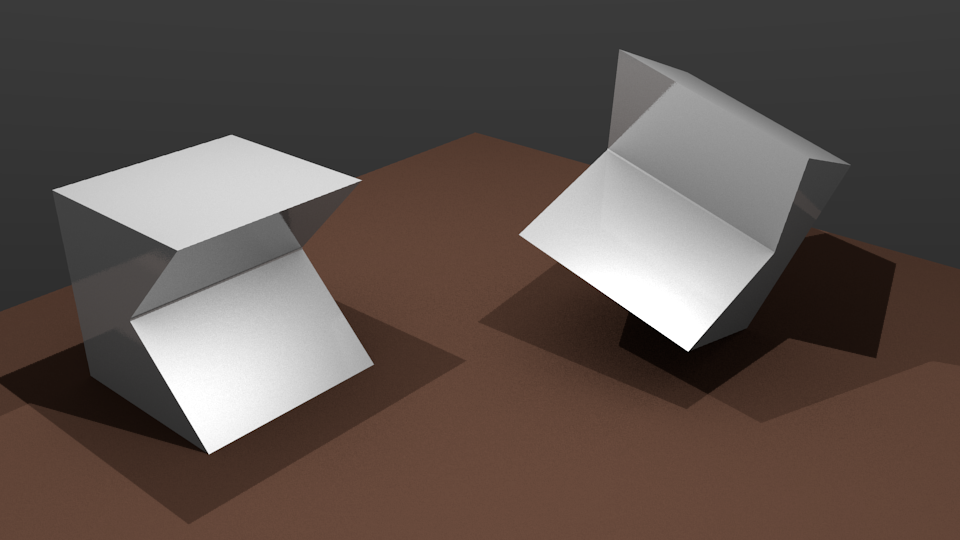
\includegraphics[width=\textwidth]{rooftop_render}
    \caption{Computer-generated rendering of two rooftop mirrors.}
    \label{fig:rooftop_render}
\end{figure}

A rooftop mirror at normal incidence can be seen as a one-port network.
Its block scattering matrix is
\begin{equation}
    \matrcp{S} =
    \begin{pmatrix}
        \matrcp{r}
    \end{pmatrix}
\end{equation}
where $\matrcp{r}$ is the reflection coefficient of the rooftop mirror.
Assuming a wave propagating toward $+\vectu{z}$ (see~\cref{fig:rooftop_imperfect}) and a rooftop mirror whose surfaces intersect along~$\vectu{x}$,
its ideal reflection coefficient is
\begin{equation}
    \matrcp{r} =
    \begin{pmatrix}
        1 &  0 & ?\\
        0 & -1 & ?\\
        ? &  ? & ?
    \end{pmatrix}
    \text{.}
\end{equation}
The question marks represent parameters that do not matter since the electric field has no component along~$\vectu{z}$.
An incident wave polarized at~\SI{45}{\degree} sees its polarization rotated by~\SI{90}{\degree} upon reflection:
\begin{align}
    \vectcp{a}_1
    &=
    \begin{pmatrix}
        \cp{\alpha} \\ \cp{\alpha} \\ 0
    \end{pmatrix}
    &
    \vectcp{b}_1
    &= \matrcp{r} \vectcp{a}_1
    =
    \begin{pmatrix}
        \cp{\alpha} \\ -\cp{\alpha} \\ 0
    \end{pmatrix}
    \text{.}
\end{align}
This is true for a perfect rooftop mirror.

The rooftop mirrors in HIFI are not perfect.
They are made out of a metal with a finite conductivity.
Furthermore, they are milled from a single block which limits the perfection of the intersection of the two plane surfaces.
\Cref{fig:rooftop_photo} shows that where the planes should intersect at right angle, there is actually a smooth curve, the radius of which corresponds to that of the milling tool.
Part of this curve forms a mirror at normal incidence.
\begin{figure}
    \centering
    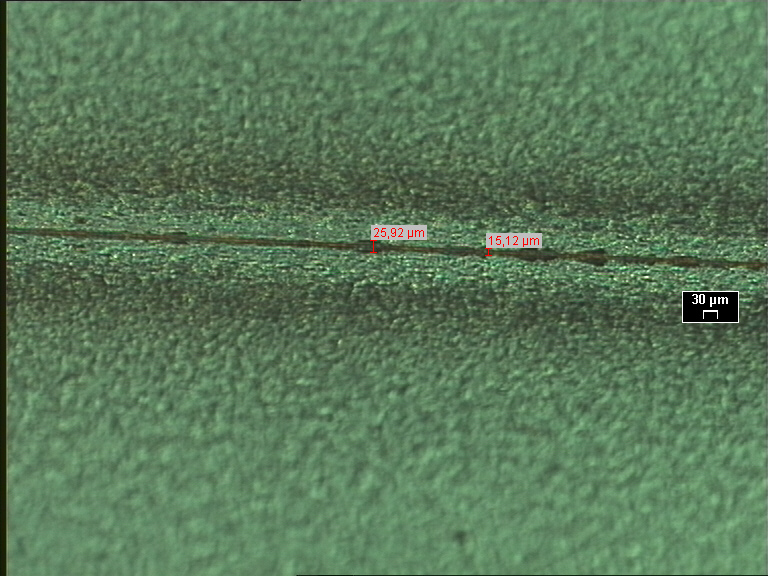
\includegraphics[width=.5\textwidth]{rooftop_front}%
    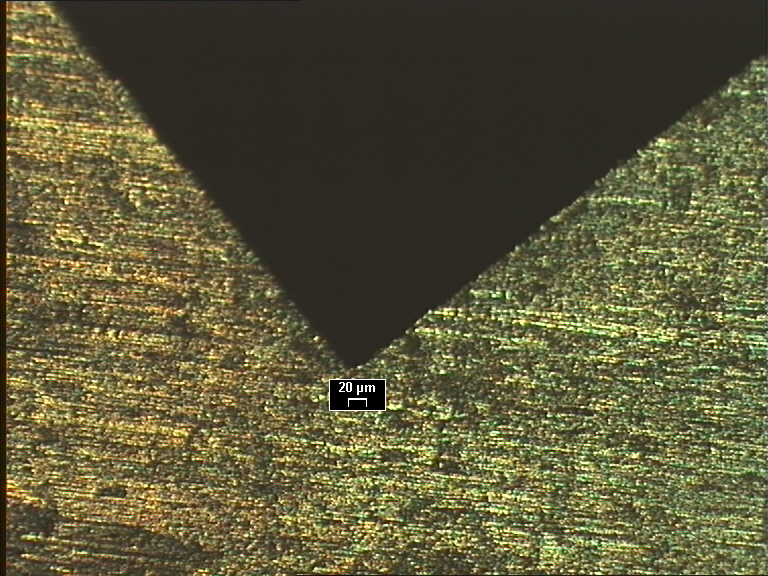
\includegraphics[width=.5\textwidth]{rooftop_side}
    \caption{Photographs of the intersection of the planes of a HIFI rooftop mirror.}
    \label{fig:rooftop_photo}
\end{figure}

The imperfection at the intersection of the two main surfaces can be approximated with a plane normal to the direction of propagation, shown in~\cref{fig:rooftop_imperfect}.
The polarization of the electric field incident to that plane is not rotated.
\begin{figure}
    \centering
    \input{rooftop_imperfect.pdf_tex}
    \caption{Side and front view of a rooftop mirror with an imperfect intersection modeled as a plane interface.}
    \label{fig:rooftop_imperfect}
\end{figure}

\Cref{fig:rooftop_networks} illustrates how one can model a more realistic rooftop mirror.
The rooftop mirror is divided into three plane metal/vacuum interfaces: two for the oblique surfaces, and one for the imperfect intersection.
Each interface forms its own network and can be modeled with the method presented in~\cref{sec:interface_between_two_media}.

A fourth network divides the incident wave in three: the incident wave shines on the three interfaces simultaneously, but each surface receives a power that is proportional to its coupling to the wave (related to its surface area).
In the other direction, the three contributions to the wave are added together.

\begin{figure}
    \centering
    \input{rooftop_networks.pdf_tex}
    \caption{Network modeling of an imperfect rooftop mirror.}
    \label{fig:rooftop_networks}
\end{figure}

\begin{samepage}
For example, the imperfection couples~\SI{1}{\percent} of the incoming power and scatters another \SI{3}{\percent} out of the system.
The remaining~\SI{96}{\percent} are shared evenly between the two oblique surfaces.
Under these conditions, the block scattering matrix of the network is
\begin{equation}
    \matrcp{S}
    =
    \begin{pmatrix}
        0 & \matr{I}_3 & \matr{I}_3 & \matr{I}_3\\
        \sqrt{.48}\,\matr{I}_3 & 0 & 0 & 0\\ 
        \sqrt{.01}\,\matr{I}_3 & 0 & 0 & 0\\
        \sqrt{.48}\,\matr{I}_3 & 0 & 0 & 0
    \end{pmatrix}
\end{equation}
in which~$\matr{I}_3$ is the identity matrix of rank~3.
\end{samepage}



%=============================================================================

\subsection{Distributed interface}

The interfaces described in the previous sections are clearly localized, they are are planar and their reflection coefficient matches that of the material.

Some components, on the other hand, have their reflection coefficient distributed over a more complicated shape.
For example, \cref{fig:distributed_interface} presents the geometry of a corrugated horn.
Those are used in the mixer sub-assemblies of HIFI, they smooth the impedance transition between the optical and the microwave sides of the instrument.
The HIFI mixers are located at the apex of the horn (``antenna'' on the figure).

A simple way to model such a complex element is to consider its ``effective reflection coefficient''.
The effective reflection coefficient is the reflection coefficient that a plane interface would need to have in order to have the same scattering matrix.
This effective reflection coefficient depends on the location of this effective interface.
We are free to choose any convenient location;
for example, in the case of a horn, one can choose to locate the effective interface at the mouth or the apex.

\begin{figure}
    \centering
    \input{distributed_itnterface.pdf_tex} % Yup, typo in the file name
    \caption{
        Every point of the surface of a corrugated horn might reflect the electric field
        that it receives.
        The arrows illustrate that the total reflection coefficient of the horn
        is a contribution of several (or even many) local reflection coefficients.
        The arrows do not represent rays or paths.
    }
    \label{fig:distributed_interface}
\end{figure}

The effective reflection coefficient of a distributed interface could be calculated by performing a finite-element analysis.
Alternatively, it can be left as a free parameter and determined by fitting the model to experimental data.

The effective reflection coefficient of a distributed interface is likely to be frequency-dependent.
Without an accurate model for every frequency, one should expect to see slight disagreements between the simulations and reality.



%=============================================================================

\subsection{Wire grid polarizer}
\label{sec:wire_grid_polarizer}
\Textcite{houde_2001} present a set of equations modeling the effect of a wire-grid polarizer on the intensity, polarization, phase and direction of a plane wave.
That work makes the following assumptions:
\begin{itemize}[noitemsep]
    \item The surrounding propagation medium is vacuum.
    \item The incident wave is plane and homogeneous.
    \item The grid contains an infinite amount of infinitely long wires, all parallel and coplanar.
    \item The wires are free floating (no thin-film dielectric substrate).
    \item The wires have a cylindrical cross-section.
    \item The radius of the wires is much smaller than the wavelength of the incident wave.
    \item The conductivity of the wires is very high, so that the electric field does not penetrate deeply inside the wires (the currents are described by a Dirac distribution to remain exactly on the surface of the wires).
    \item The results are computed for the far field.
    \item We are in a steady periodic state (the angular frequency is real), which means that this grid model cannot be used with time-varying inputs (see~\cref{sec:complex_angular_frequency}).
\end{itemize}

\begin{figure}
    \centering
    \footnotesize
    \input{grid.pdf_tex}
    \caption{A free-floating wire grid polarizer, its dimensions and its local reference frame.}
    \label{fig:grid}
\end{figure}

\subsubsection{Reflection and transmission coefficients}
In this section, we rewrite some equations from~\textcite{houde_2001} in order to express them as Jones matrices.

The set of equations that interest us are the equations numbered 23, 24 and 30 to 35 in the article, which we reproduce here for convenience.
The notations are explained in the article, we will not explain them here.
The first two equations, \eqref{eq:grid_current_linear} and \eqref{eq:grid_current_circular}, describe the electric current at the surface of the wires.
$K^x$ corresponds to a linear current and $K^\theta$ to a circular current.
In the first case, electrons move along the length of the wire; in the other, they rotate around the axis of the wire.
\begin{align}
    K^x &= \frac{E_0}{F} \cdot \alpha' \frac{N_x}{\Delta_x}
    \label{eq:grid_current_linear}
    \\
    K^\theta &= (-i) \frac{E_0}{F} \cdot (\gamma' \beta - \beta' \gamma) \frac{N_\theta}{\Delta_\theta}
    \label{eq:grid_current_circular}
\end{align}
In these equations, $E_0$ is the amplitude of the electric field, $F$ a constant (the value of which does not matter because it disappears from the equations at a later stage).
$(\alpha, \beta, \gamma)\transp$ is the direction of the wave vector and
$(\alpha', \beta', \gamma')\transp$ is the direction of the electric field.
The parameters $N_x$, $\Delta_x$, $N_\theta$ and $\Delta_\theta$ encode the effect of the geometry of the grid and the angle of incidence.

The following equations describe the components of the reflected and transmitted fields in the reference frame of the grid.
\begin{align}
    r_{xg}
    &=
    -\frac{F}{E_0}
    \frac{\lambda}{\pi d}
    \frac{1 - \alpha^2}{\gamma} K^x
    \label{eq:houde_Rx}
    \\
    r_{yg}
    &=
    \phantom{-}
    \frac{F}{E_0}
    \frac{\lambda}{\pi d}
    \left(
        \frac{\alpha \beta}{\gamma} K^x
        -
        i \frac{ka}{2} K^\theta
    \right)
    \\
    r_{zg}
    &=
    -\frac{F}{E_0}
    \frac{\lambda}{\pi d}
    \left(
       \alpha K^x
       +
       i \frac{\beta}{\gamma} \frac{ka}{2} K^\theta
    \right)
    \\
    t_{xg} &= \alpha' + r_{xg}
    \\
    t_{yg}
    &=
    \beta' +
    \frac{F}{E_0}
    \frac{\lambda}{\pi d}
    \left(
        \frac{\alpha \beta}{\gamma} K^x + i \frac{ka}{2} K^\theta
    \right)
    \\
    t_{zg}
    &=
    \gamma' +
    \frac{F}{E_0}
    \frac{\lambda}{\pi d}
    \left(
        \alpha K^x - i \frac{\beta}{\gamma} \frac{ka}{2} K^\theta
    \right)
\end{align}
We use the subscript~``$g$'' to remind us that these are valid in the reference frame of the grid.
Note that \citeauthor{houde_2001} call these $r$ and $t$ ``reflection'' and ``transmission coefficient'', something they are not quite since they contain $\alpha'$, $\beta'$ and $\gamma'$, which correspond to the intensity of the incoming electric field in the three dimensions: $\vect{e}_g=E_0 (\alpha' \: \beta' \: \gamma')\transp$.
These amplitudes have to be factored out if we want actual reflection and transmission coefficients.

When examining these equations, some simplifications are obvious.
For example, $\frac{E_0}{F}$ inside $K^x$ and $K^\theta$ cancels $\frac{F}{E_0}$ in $r$ and $t$;
the complex unit~$i$ within $K^\theta$ combines with $i$ in $r$ and $t$ to become~$-1$.

In these equations, $\alpha'$, $\beta'$ and $\gamma'$ are the three components of the direction of the incident electric field vector, satisfying $\alpha'^2 + \beta'^2 + \gamma'^2 = 1$.
That condition seems to apply only to real numbers, restricting the use of this grid model to waves that are linearly polarized (their three components are in phase).
However, there is no such limitation in the model.
Indeed, the authors define the incident electric field as
$(e_{xg} \: e_{yg} \: e_{zg})\transp = E_0(\alpha' \: \beta' \: \gamma')\transp$.
The amplitude $E_0$ can be complex which makes its phase common to the three components.
When we rewrite the equations in a matrix form, we notice that the actual parameters that matter are not $\alpha'$, $\beta'$, $\gamma'$ and $E_0$, but $e_{xg}$, $e_{yg}$ and $e_{zg}$ themselves, all of which can have their own phase.
Consequently, the model also applies to elliptically-polarized waves.

In order to rewrite these equations in a matrix form, one needs to split each coefficient of transmission and reflection into three components like this:
\begin{equation}
    e_{\R xg} = r_{xxg} e_{xg} + r_{xyg} e_{yg} + r_{xzg} e_{zg}
\end{equation}
so that we can write
\begin{align}
    \vect{e}_{\R g} &= \matr{r}_g \vect{e}_{\I g}
    \\
    \vect{e}_{\R g} &=
    \begin{pmatrix}
        r_{xxg} & r_{xyg} & r_{xzg} \\
        r_{yxg} & r_{yyg} & r_{yzg} \\
        r_{zxg} & r_{zyg} & r_{zzg}
    \end{pmatrix}
    \vect{e}_{\I g}
\end{align}
for the reflection $\matr{r}_g$ and a similar equation
for the transmission $\vect{e}_{\T g} = \matr{t}_g \vect{e}_{\I g}$.
We start with $r_{xg}$ defined in \cref{eq:houde_Rx} to get $r_{xxg}$, $r_{xyg}$ and $r_{xzg}$.
\begin{align*}
    e_{\R xg} &= r_{xg} E_0
    \\
           &= -\frac{F}{E_0}
              \frac{\lambda}{\pi d}
              \frac{1-\alpha^2}{\gamma}
              K^x
              E_0
    \\
           &= -\cancel{\frac{F}{E_0}}
              \frac{\lambda}{\pi d}
              \frac{1-\alpha^2}{\gamma}
              \cancel{\frac{E_0}{F}}
              \frac{N_x}{\Delta_x}
              \underbrace{
                  \alpha'
                  E_0
              }_{e_{\I xg}}
    \\
           &= -\frac{\lambda}{\pi d}
              \frac{1-\alpha^2}{\gamma}
              \frac{N_x}{\Delta_x}
              e_{\I xg}
\end{align*}
By identification, we find these values for $r_{xxg}$, $r_{xyg}$ and $r_{xzg}$.
\begin{equation}
    \left\lbrace
    \begin{aligned}
        r_{xxg} &= -\frac{\lambda}{\pi d}
                  \frac{N_x}{\Delta_x}
                  \frac{1-\alpha^2}{\gamma}
        \\
        r_{xyg} &= 0
        \\
        r_{xzg} &= 0
    \end{aligned}
    \right.
\end{equation}
Let us continue with $r_{yg}$,
\begin{align*}
    e_{\R yg}
    &= r_{yg} E_0
    \\
    &= \frac{F}{E_0}
       \frac{\lambda}{\pi d}
       \left(
           \frac{\alpha \beta}{\gamma}
           K^x
           -
           i
           \frac{ka}{2}
           K^\theta           
       \right)
       E_0
    \\
    &= \cancel{\frac{F}{E_0}}
       \frac{\lambda}{\pi d}
       \left(
           \frac{\alpha \beta}{\gamma}
           \cancel{\frac{E_0}{F}}
           \frac{N_x}{\Delta_x}
           \alpha'
           -
           i
           \frac{ka}{2}
           (-i)
           \cancel{\frac{E_0}{F}}
           \frac{N_\theta}{\Delta_\theta}
           (\gamma' \beta - \beta' \gamma)           
       \right)
       E_0
    \\
    &= \frac{\lambda}{\pi d}
       \left(
           \frac{\alpha \beta}{\gamma}
           \frac{N_x}{\Delta_x}
           \alpha'
           +
           \frac{ka}{2}
           \frac{N_\theta}{\Delta_\theta}
           \gamma
           \beta'
           -
           \frac{ka}{2}
           \frac{N_\theta}{\Delta_\theta}
           \beta
           \gamma'
       \right)
       E_0
    \\
    &= \frac{\lambda}{\pi d}
       \frac{\alpha \beta}{\gamma}
       \frac{N_x}{\Delta_x}
       \underbrace{E_0 \alpha'}_{e_{\I xg}}
       +
       \frac{\lambda}{\pi d}
       \frac{ka}{2}
       \frac{N_\theta}{\Delta_\theta}
       \gamma
       \underbrace{E_0 \beta'}_{e_{\I yg}}
       -
       \frac{\lambda}{\pi d}
       \frac{ka}{2}
       \frac{N_\theta}{\Delta_\theta}
       \beta
       \underbrace{E_0 \gamma'}_{e_{\I zg}}
\end{align*}
\begin{equation}
    \left\lbrace
    \begin{aligned}
        r_{yxg}
        &=
        \phantom{-}
        \frac{\lambda}{\pi d}
        \frac{N_x}{\Delta_x}
        \frac{\alpha \beta}{\gamma}
        \\
        r_{yyg}
        &=
        \phantom{-}
        \frac{\lambda}{\pi d}
        \frac{N_\theta}{\Delta_\theta}
        \frac{ka}{2}
        \gamma
        \\
        r_{yzg}
        &=
        -
        \frac{\lambda}{\pi d}
        \frac{N_\theta}{\Delta_\theta}
        \frac{ka}{2}
        \beta
    \end{aligned}
    \right.
\end{equation}
and similarly for $r_{zg}$,
\begin{align*}
    e_{\R zg} &= r_{zg} E_0
    \\
    &=
    -
    \frac{F}{E_0}
    \frac{\lambda}{\pi d}
    \left(
        \alpha K^x
        +
        i
        \frac{\beta}{\gamma}
        \frac{ka}{2}
        k^\theta
    \right)
    E_0
    \\
    &=
    -
    \cancel{\frac{F}{E_0}}
    \frac{\lambda}{\pi d}
    \left(
        \alpha
        \cancel{\frac{E_0}{F}}
        \frac{N_x}{\Delta_x}
        \alpha'
        +
        i
        \frac{\beta}{\gamma}
        \frac{ka}{2}
        (-i)
        \cancel{\frac{E_0}{F}}
        (\gamma' \beta - \beta' \gamma)
        \frac{N_\theta}{\Delta_\theta}
    \right)
    E_0
    \\
    &=
    -
    \frac{\lambda}{\pi d}
    \alpha
    \frac{N_x}{\Delta_x}
    \underbrace{E_0 \alpha'}_{e_{\I xg}}
    +
    \frac{\lambda}{\pi d}
    \frac{\beta}{\gamma}
    \frac{ka}{2}
    \frac{N_\theta}{\Delta_\theta}
    \gamma
    \underbrace{E_0 \beta'}_{e_{\I yg}}
    -
    \frac{\lambda}{\pi d}
    \frac{\beta}{\gamma}
    \frac{ka}{2}
    \frac{N_\theta}{\Delta_\theta}
    \beta
    \underbrace{E_0 \gamma'}_{e_{\I zg}}
\end{align*}
\begin{equation}
    \left\lbrace
    \begin{aligned}
        r_{zxg}
        &=
        -
        \frac{\lambda}{\pi d}
        \frac{N_x}{\Delta_x}
        \alpha
        \\
        r_{zyg}
        &=
        \phantom{-}
        \frac{\lambda}{\pi d}
        \frac{N_\theta}{\Delta_\theta}
        \frac{ka}{2}
        \beta
        \\
        r_{zzg}
        &=
        -
        \frac{\lambda}{\pi d}
        \frac{N_\theta}{\Delta_\theta}
        \frac{ka}{2}
        \frac{\beta^2}{\gamma}
    \end{aligned}
    \right.
\end{equation}
Hence, we have derived the nine parameters of the reflection coefficient matrix.
Next, we compute the transmission matrix.
\begin{align*}
    e_{\T xg} &= t_{xg} E_0
    \\
    &= (\alpha' + r_{xg}) E_0
    \\
    &= \underbrace{\alpha' E_0}_{e_{\I xg}}
       -
       \frac{\lambda}{\pi d}
       \frac{1 - \alpha^2}{\gamma}
       \frac{N_x}{\Delta_x}
       \underbrace{\alpha' E_0}_{e_{\I xg}}
    \\
    &= \left(
           1
           -
           \frac{\lambda}{\pi d}
           \frac{1 - \alpha^2}{\gamma}
           \frac{N_x}{\Delta_x}
       \right)
       e_{\I xg}
\end{align*}
\begin{equation}
    \left\lbrace
    \begin{aligned}
        t_{xxg}
        &= 1
           -
           \frac{\lambda}{\pi d}
           \frac{N_x}{\Delta_x}
           \frac{1 - \alpha^2}{\gamma}
        \\
        t_{xyg} &= 0
        \\
        t_{xzg} &= 0
    \end{aligned}
    \right.
\end{equation}

\begin{align*}
    e_{\T yg} &= t_{yg} E_0
    \\
    &=
    \left(
        \beta'
        +
        \frac{F}{E_0}
        \frac{\lambda}{\pi d}
        \left[
            \frac{\alpha \beta}{\gamma}
            K^x
            +
            i
            \frac{ka}{2}
            K^\theta
        \right]
    \right)
    E_0
    \\
    &=
    \left(
        \beta'
        +
        \cancel{\frac{F}{E_0}}
        \frac{\lambda}{\pi d}
        \left[
            \frac{\alpha \beta}{\gamma}
            \cancel{\frac{E_0}{F}}
            \frac{N_x}{\Delta_x}
            \alpha'
            +
            i
            \frac{ka}{2}
            (-i)
            \cancel{\frac{E_0}{F}}
            \frac{N_\theta}{\Delta_\theta}
            (\gamma' \beta - \beta' \gamma)
        \right]
    \right)
    E_0
    \\
    &=
    \left(
        \beta'
        +
        \frac{\lambda}{\pi d}
        \frac{\alpha \beta}{\gamma}
        \frac{N_x}{\Delta_x}
        \alpha'
        -
        \frac{\lambda}{\pi d}
        \frac{ka}{2}
        \frac{N_\theta}{\Delta_\theta}
        \gamma
        \beta'
        +
        \frac{\lambda}{\pi d}
        \frac{ka}{2}
        \frac{N_\theta}{\Delta_\theta}
        \beta
        \gamma'
    \right)
    E_0
    \\
    &=
    \frac{\lambda}{\pi d}
    \frac{\alpha \beta}{\gamma}
    \frac{N_x}{\Delta_x}
    \underbrace{E_0 \alpha'}_{e_{\I xg}}
    +
    \left(
        1
        -
        \frac{\lambda}{\pi d}
        \frac{ka}{2}
        \frac{N_\theta}{\Delta_\theta}
        \gamma
    \right)
    \underbrace{E_0 \beta'}_{e_{\I yg}}
    +
    \frac{\lambda}{\pi d}
    \frac{ka}{2}
    \frac{N_\theta}{\Delta_\theta}
    \beta
    \underbrace{E_0 \gamma'}_{e_{\I zg}}
\end{align*}
\begin{equation}
    \left\lbrace
    \begin{aligned}
        t_{yxg}
        &= \frac{\lambda}{\pi d}
           \frac{N_x}{\Delta_x}
           \frac{\alpha \beta}{\gamma}
        \\
        t_{yyg}
        &= 1
           -
           \frac{\lambda}{\pi d}
           \frac{N_\theta}{\Delta_\theta}
           \frac{ka}{2}
           \gamma
        \\
        t_{yzg}
        &= \frac{\lambda}{\pi d}
           \frac{N_\theta}{\Delta_\theta}
           \frac{ka}{2}
           \beta
    \end{aligned}
    \right.
\end{equation}

\begin{align*}
    e_{\T zg} &= t^{zg} E_0
    \\
    &=
    \left(
        \gamma' +
        \frac{F}{E_0}
        \frac{\lambda}{\pi d}
        \left[
            \alpha K^x - i \frac{\beta}{\gamma} \frac{ka}{2} K^\theta
        \right]
    \right)
    E_0
    \\
    &=
    \left(
        \gamma' +
        \cancel{\frac{F}{E_0}}
        \frac{\lambda}{\pi d}
        \left[
            \alpha
            \cancel{\frac{E_0}{F_0}}
            \frac{N_x}{\Delta_x}
            \alpha'
            -
            i
            \frac{\beta}{\gamma}
            \frac{ka}{2}
            (-i)
            \cancel{\frac{E_0}{F}}
            \frac{N_\theta}{\Delta_\theta}
            (\gamma' \beta - \beta' \gamma)
        \right]
    \right)
    E_0
    \\
    &=
    \left(
        \gamma' +
        \frac{\lambda}{\pi d}
        \left[
            \alpha
            \frac{N_x}{\Delta_x}
            \alpha'
            +
            \frac{\beta}{\gamma}
            \frac{ka}{2}
            \frac{N_\theta}{\Delta_\theta}
            \gamma
            \beta'
            -
            \frac{\beta}{\gamma}
            \frac{ka}{2}
            \frac{N_\theta}{\Delta_\theta}
            \beta
            \gamma'
        \right]
    \right)
    E_0
    \\
    &=
    \frac{\lambda}{\pi d}
    \alpha
    \frac{N_x}{\Delta_x}
    \underbrace{E_0 \alpha'}_{e_{\I xg}}
    +
    \frac{\lambda}{\pi d}
    \frac{\beta}{\gamma}
    \frac{ka}{2}
    \frac{N_\theta}{\Delta_\theta}
    \gamma
    \underbrace{E_0 \beta'}_{e_{\I yg}}
    +
    \left(
        1
        -
        \frac{\lambda}{\pi d}
        \frac{\beta}{\gamma}
        \frac{ka}{2}
        \frac{N_\theta}{\Delta_\theta}
        \beta
    \right)
    \underbrace{E_0 \gamma'}_{e_{\I zg}}
\end{align*}
\begin{equation}
    \left\lbrace
    \begin{aligned}
        t_{zxg}
        &= \frac{\lambda}{\pi d}
           \frac{N_x}{\Delta_x}
           \alpha
        \\
        t_{zyg}
        &= \frac{\lambda}{\pi d}
           \frac{N_\theta}{\Delta_\theta}
           \frac{ka}{2}
           \frac{\beta}{\gamma}
           \gamma
        \\
        t_{zzg}
        &= 1
           -
           \frac{\lambda}{\pi d}
           \frac{N_\theta}{\Delta_\theta}
           \frac{ka}{2}
           \frac{\beta}{\gamma}
           \beta
    \end{aligned}
    \right.
\end{equation}

With another simplification,
\begin{equation}
    k = 2\pi / \lambda
    \quad \Rightarrow \quad
    \frac{\lambda}{\pi d} \frac{ka}{2}
    =
    \frac{\lambda}{\pi d} \frac{2\pi a}{2\lambda}
    =
    \frac{a}{d}
\end{equation}
the matrix form of the reflection and transmission coefficients reduces to
\begin{equation}
    \matr{r}_g =
    \begin{pmatrix}
        -\frac{\lambda}{\pi d}
        \frac{N_x}{\Delta_x}
        \frac{1 - \alpha^2}{\gamma}
        &
        0
        &
        0
        \\
        \frac{\lambda}{\pi d}
        \frac{N_x}{\Delta_x}
        \frac{\alpha \beta}{\gamma}
        &
        \frac{a}{d}
        \frac{N_\theta}{\Delta_\theta}
        \gamma
        &
        -
        \frac{a}{d}
        \frac{N_\theta}{\Delta_\theta}
        \beta
        \\
        -
        \frac{\lambda}{\pi d}
        \frac{N_x}{\Delta_x}
        \alpha
        &
        \frac{a}{d}
        \frac{N_\theta}{\Delta_\theta}
        \beta
        &
        -
        \frac{a}{d}
        \frac{N_\theta}{\Delta_\theta}
        \frac{\beta^2}{\gamma}
    \end{pmatrix}
    \label{eq:grid_rg}
\end{equation}
and
\begin{equation}
    \matr{t}_g =
    \begin{pmatrix}
        1 -
        \frac{\lambda}{\pi d}
        \frac{N_x}{\Delta_x}
        \frac{1 - \alpha^2}{\gamma}
        &
        0
        &
        0
        \\
        \frac{\lambda}{\pi d}
        \frac{N_x}{\Delta_x}
        \frac{\alpha \beta}{\gamma}
        &
        1 -
        \frac{a}{d}
        \frac{N_\theta}{\Delta_\theta}
        \gamma
        &
        \frac{a}{d}
        \frac{N_\theta}{\Delta_\theta}
        \beta
        \\
        \frac{\lambda}{\pi d}
        \frac{N_x}{\Delta_x}
        \alpha
        &
        \frac{a}{d}
        \frac{N_\theta}{\Delta_\theta}
        \beta
        &
        1 -
        \frac{a}{d}
        \frac{N_\theta}{\Delta_\theta}
        \frac{\beta^2}{\gamma}
    \end{pmatrix}
    \text{.}
    \label{eq:grid_tg}
\end{equation}
These reflection and transmission matrices are three-dimensional Jones matrices.

In these matrices, the parameter $a$ is the radius of the wires
and $d$ is the axis-to-axis distance between the wires.
Because the incident wave is homogeneous and propagating in a lossless medium (vacuum), $\vectcp{k}_1$ is actually a real vector: $\vectcp{k}_1 = \vect{k}_1$.
Therefore it has an associated real wave number~$k$
\begin{equation}
    k = \norm{\vect{k}_1}\text{.}
\end{equation}
The wavelength $\lambda$ that appears in the matrices is given by
\begin{equation}
    \lambda = \frac{2 \pi}{k}
    \text{.}
\end{equation}
The direction of propagation of the incident wave is
\begin{equation}
    \vectu{k}_1 = \frac{1}{k} \vect{k}_1
    \text{.}
\end{equation}
It defines the values $\alpha$, $\beta$ and $\gamma$ that appear in the matrices:
\begin{equation}
    \begin{pmatrix}
    \alpha \\ \beta \\ \gamma
    \end{pmatrix}
    =
    \vectu{k}_1
\end{equation}

The parameters $N_x$, $\Delta_x$, $N_\theta$ and $\Delta_\theta$ are given by \textcite{houde_2001}:
\begin{align}
    N_x
    &=
    1 - i \frac{\cp{Z}_s}{Z_0} \frac{ka}{2}
    \\
    N_\theta
    &=
    1 + i \frac{\cp{Z}_s}{Z_0} \frac{2}{ka}
\end{align}
\begin{multline}
    \Delta_x \approx
    (1-\alpha)^2
    \left[
        \left\lbrace
            \frac{\lambda}{\pi \gamma d}
            -
            \left(
                \frac{k'a}{2}
            \right)^2
            +
            \frac{
                1
            }{
                \sqrt{
                    \pi
                    (1 - \alpha)^2
                    Z_0
                    \sigma
                    \lambda
                }
            }
            \left(
                \frac{2}{k'a}
            \right)
        \right\rbrace
    \right.
    \\
        +i \frac{2}{\pi}
        \left\lbrace
            \ln \left( \frac{d}{2\pi a} \right)
            +
            \frac{\pi^2}{6}
            \left(
                \frac{d \gamma}{\lambda}
            \right)^2
            -
            \left(
                \frac{k'a}{2}
            \right)^2
            \left[
                1 - \Psi - \ln\left( \frac{k'a}{2} \right)
            \right]
        \right.
            +
    \\
    \left.
        \left.
            \sqrt{
                \frac{\pi}{
                    4
                    (1-\alpha)^2
                    Z_0
                    \sigma
                    \lambda
                }
            }
            \frac{2}{k'a}
        \right\rbrace
    \right]
\end{multline}
\begin{equation}
    \Delta_\theta
    \approx
    -(1-\alpha)^2
    \frac{\cp{Z}_s}{Z_0}
    \frac{2}{\pi}
    \ln \left(
        \frac{2}{2\pi a}
    \right)
    +
    i
    \left\lbrace
        \frac{\lambda}{\pi^2 a}
        +
        (1-\alpha^2)
        \frac{\cp{Z}_s}{Z_0}
        \frac{\lambda}{\pi \gamma d}
    \right\rbrace
\end{equation}
where $\Psi$ is Euler's constant (\num{0.577}\dots), $k'= k \sqrt{1-\alpha^2}$ and
\begin{equation}
    \cp{Z}_s = (1 + i) \sqrt{\frac{\mu_0 \omega}{2 \sigma}}
\end{equation}
is the wave impedance at the surface of the wire.
This expression is merely a complicated way to write
$\cp{Z}_s = \sqrt{\mu_0 / \cp{\epsilon}}$ with $\cp{\epsilon}=-i \sigma / \omega$.
The minus sign is a consequence of the convention chosen by~\citeauthor{houde_2001}.
Before using these equations, we must adapt the two conventions.

\subsubsection{Sign conventions}
We need to adapt the conventions of~\textcite{houde_2001} to that of our model.
We use the physics convention
$\vectcp{E}=\vectcp{e} \exp[i(\vectcp{k}\cdot \vect{r} - \cp{\omega}t)]$
while \citeauthor{houde_2001} use the engineering convention
$\vectcp{E}=\vectcp{e} \exp[i(-\vectcp{k}\cdot \vect{r} + \cp{\omega}t)]$.
Both conventions must describe the same physical phenomenon.
The actual physical phenomenon studied here is a
real electric field~$\vect{E} = \Re(\vectcp{E})$.
In order to describe that same real phenomenon, the wave vectors in each convention must be complex conjugates of each other.
Likewise, the complex angular frequency in one convention is the complex conjugate of the other.
In order to use \cref{eq:grid_rg,eq:grid_tg}, we must take the complex conjugate of the incident wave vector and of the angular frequency.

In \textcite{houde_2001}, the surrounding medium is lossless and the incident wave is homogeneous, therefore the wave vector is real and is equal to its conjugate.
However, the wave vector in the metallic wire has an imaginary part linked to the conductivity of the medium.
Since the \citeauthor{houde_2001} assume that the angular frequency and the magnetic permeabilities are real, it is sufficient to flip the sign of this conductivity: we must replace $\sigma$ with $-\sigma$ in the equations.
In particular, $\cp{Z}_s = \sqrt{\mu_0 / \cp{\epsilon}}$ must use
$\cp{\epsilon} = -i (-\sigma) / \omega$.

%-----------------------------------------------------------------------------
\subsubsection{Scattering matrix}
A grid at oblique incidence is modeled by a four-port network.
Its block scattering matrix in the reference frame of the grid is
\begin{equation}
    \matrcp{S}_g
    =
    \begin{pmatrix}
        0               & \matrcp{r}_{2g} & \matrcp{t}_{3g} & 0               \\
        \matrcp{r}_{1g} & 0               & 0               & \matrcp{t}_{4g} \\
        \matrcp{t}_{1g} & 0               & 0               & \matrcp{r}_{4g} \\
        0               & \matrcp{t}_{2g} & \matrcp{r}_{3g} & 0
    \end{pmatrix}
    \label{eq:grid_scattering_local}
\end{equation}
in which every $\matrcp{r}_{ig}$ and $\matrcp{t}_{ig}$ is a Jones matrix referring to a reflection or a transmission coefficient.

In the global reference frame, its block scattering matrix is
\begin{equation}
    \matrcp{S}
    =
    \begin{pmatrix}
        0              & \matrcp{r}_{2} & \matrcp{t}_{3} & 0               \\
        \matrcp{r}_{1} & 0              & 0              & \matrcp{t}_{4} \\
        \matrcp{t}_{1} & 0              & 0              & \matrcp{r}_{4} \\
        0              & \matrcp{t}_{2} & \matrcp{r}_{3} & 0
    \end{pmatrix}
    \text{.}
    \label{eq:grid_scattering_global}
\end{equation}
The Jones matrices in the grid and global reference frames are related by a rotation matrix~$\matr{A}$:
\begin{equation}
    \matrcp{S}_{ij} = \matr{A} \matrcp{S}_{ijg} \matr{A}^{-1}
    \text{.}
    \label{eq:grid_rotation}
\end{equation}
See~\cref{sec:rotating_jones_matrices} for a brief note on rotating Jones matrices.

\citeauthor{houde_2001} define the following reference frame for the grid: the wires are along $\vectu{x}_g=(1 \; 0 \; 0)\transp$ and the normal to the grid is $\vectu{z}_g=(0 \; 0 \; 1)\transp$ (see~\cref{fig:grid}).
They also present another reference frame called ``the laboratory reference frame'' but it is not useful for us:
it actually consists of two reference frames, one for the incident and transmitted waves and one for the reflected wave; it is not a global reference frame.

In the global reference frame,
%the wires of the grid are along the vector~$\matr{A} (1 \; 0 \; 0)\transp$ and
the normal of the grid is $\vectu{n} = \matr{A} (0 \; 0 \; 1)\transp$.
Since a grid is a four-port device not unlike an interface at oblique incidence, we use the notations and indices of~\cref{fig:network_interface}:
Port~1 reflects to Port~2 and transmits to Port~3.
$\vect{k}_1$ is the wave vector of the wave incident to Port~1,
$\vect{k}_2$ is the wave vector of the wave incident to Port~2, etc.

The normal component of $\vect{k}_1$ and $\vect{k}_2$ is positive: the waves incident to Ports~1 and 2 propagate along the normal, not against it.
The normal component of $\vect{k}_3$ and $\vect{k}_4$ is negative.
This point is important: the equations modeling the grid are not symmetrical.
These equations assume that the incident wave propagates in the direction of the normal to the grid ($\vect{k} \cdot \vectu{n} >= 0$)
which is true for Ports~1 and ~2 but not for Ports~3 and~4.
If we apply the grid equations to a wave propagating the wrong direction, the grid equations create energy instead of absorbing and splitting it, which is not physical.
To determine the reflection and transmission coefficients of Ports~3 and~4,
it is sufficient to calculate
$\matrcp{r}_{1g}$, $\matrcp{t}_{1g}$, $\matrcp{r}_{2g}$ and $\matrcp{t}_{2g}$.
By symmetry,
$\matrcp{r}_{3g}=\matrcp{r}_{1g}$,
$\matrcp{t}_{3g}=\matrcp{t}_{1g}$,
$\matrcp{r}_{4g}=\matrcp{r}_{2g}$ and
$\matrcp{t}_{4g}=\matrcp{t}_{2g}$.

From Snell's law, we obtain $\vect{k}_2$ by flipping the sign of the tangential component.
More precisely, we flip the sign of the normal component to account for the reflection, and subsequently flip the sign of the whole vector to make it incident onto the grid.
Then, because the propagation medium is the same on both sides of the grid, we have
$\vectcp{k}_3 = -\vectcp{k}_1$ and
$\vectcp{k}_4 = -\vectcp{k}_2$.
\begin{align}
    \vect{k}_n &= (\vect{k}_1 \cdot \vectu{n}) \vectu{n} \\
    \vect{k}_t &= \vect{k}_1 - \vect{k}_n                \\
    \vect{k}_2 &= -(\vect{k}_t - \vect{k}_n)             \\
    \vect{k}_3 &= -\vect{k}_1                            \\
    \vect{k}_4 &= -\vect{k}_2
\end{align}
These are the wave vectors of the four incident waves expressed in the global reference frame.
They correspond to the following vectors expressed in the grid reference frame:
\begin{align}
    \vect{k}_{1g} &= \matr{A}^{-1} \vect{k}_1 &
    \vect{k}_{2g} &= \matr{A}^{-1} \vect{k}_2 &
    \vect{k}_{3g} &= \matr{A}^{-1} \vect{k}_3 &
    \vect{k}_{4g} &= \matr{A}^{-1} \vect{k}_4
    \text{.}
\end{align}

To compute the reflection and transmission coefficients for each port, we use the values given by~\cref{tab:grid_values}
in~\cref{eq:grid_rg,eq:grid_tg}.
\begin{table}
    \centering
    \begin{tabular}{cc}
        \toprule
        coefficient                         & $(\alpha \; \beta \; \gamma)\transp$ \\
        \midrule
        $\matrcp{r}_{1g} = \matrcp{r}_{3g}$ & $\vectu{k}_{2g}$ \\
        $\matrcp{t}_{1g} = \matrcp{t}_{3g}$ & $\vectu{k}_{3g}$ \\
        $\matrcp{r}_{2g} = \matrcp{r}_{4g}$ & $\vectu{k}_{1g}$ \\
        $\matrcp{t}_{2g} = \matrcp{t}_{4g}$ & $\vectu{k}_{2g}$ \\
        \bottomrule
    \end{tabular}
    \caption{
        Values of $\alpha$, $\beta$ and $\gamma$
        to feed to the grid equations to compute the scattering coefficients in the reference frame of the grid.
    }
    \label{tab:grid_values}
\end{table}


Once all the reflection and transmission coefficients are calculated in the reference frame of the grid, we use~\cref{eq:grid_rotation} to express them in the global reference frame.
We can then populate the scattering matrix~\cref{eq:grid_scattering_global}.

For a grid at normal incidence, we use the same technique as the one described in~\vref{sec:interface_normal_incidence}, \textit{\nameref{sec:interface_normal_incidence}} with $\vect{k}_2=-\vect{k}_1$.





%=============================================================================

\subsection{Gray body}
\label{sec:gray_body}
A black body absorbs all incoming radiation, it reflects nothing.
In thermal equilibrium, a black body of temperature $\theta$%
\footnote{
    We use $\theta$ for temperature because we reserve $T$ for transmission gain.
}
emits a spectral radiance of
\begin{equation}
    B(f, \theta) =
    \frac{2 h f^3}{c^2}
    \frac{1}{
        \exp \left(
            \frac{h f}{k_B \theta}
        \right)
        -1
    }
\end{equation}
in which $f$ the frequency, $h$ is the Planck constant, $k_B$ the Boltzmann constant and $c$ the speed of light in the medium surrounding the black body.
The SI unit of $B$ is \si{\watt\per\meter\squared\per\steradian\per\hertz}.
The total surface power density emitted by a black body is given by the Stefan--Boltzmann law
\begin{equation}
    j^\star = \sigma \theta^4
\end{equation}
in which $\sigma$ is the Stefan--Boltzmann constant and
$j^\star$ is expressed in \si{\watt\per\meter\squared}.

Black bodies do not adequately model the calibration loads of an instrument like HIFI.
Although the calibration loads are designed to minimize reflection, said reflections are never zero.
A better model for calibrations load uses gray bodies.
Gray bodies emit and reflect at the same time,
but the more they reflect, the less they emit.
For a gray body, the Stefan--Boltzmann law becomes
\begin{equation}
    j^\star = \epsilon(f) \sigma \theta^4
\end{equation}
in which $\epsilon \in [0,1]$ is called the ``emissivity'' and is function of the frequency.

The reflection gain $R$, transmission gain $T$ and absorption gain $A$ of a body are linked by
\begin{equation}
    R + T + A = 1
\end{equation}
which states that energy is conserved.
Kirchhoff's law of thermal radiation states that the emissivity of a body equals its absorption: $\epsilon = A$.
If the body is opaque, then $\T=0$ and therefore $R=1-A=1-\epsilon$.
When we express this in field and not in power, we get
\begin{equation}
    \alpha = \sqrt{ 1 - \abs{\cp{r}}^2 } \text{.}
\end{equation}
with $\cp{r}$ the coefficient of reflection and $\alpha$ the coefficient of emission such that $\alpha^2=A=\epsilon$.
These are illustrated in~\cref{fig:gray_body}.

We represent the reflective surface of the gray body with a two-port network, as shown on the right of~\cref{fig:gray_body}.
The port 1 is inside the gray body, the port 2 is outside.
Using the notations of the figure,
\begin{align}
    \cp{b}_1 &= 0 \\
    \cp{b}_2 &= \alpha \cp{a}_1 + \cp{r} \cp{a}_2
\end{align}
Here, the input $\cp{a}_1$ is the electric field emitted by an ideal black body.
The reflection and emission coefficients $\cp{r}$ and $\alpha$ transform this black body emission into a gray body emission.

\begin{figure}[b]
    \centering
    \input{gray_body.pdf_tex}
    \caption{Model of a gray body.
    $\alpha$ is a emission coefficient.}
    \label{fig:gray_body}
\end{figure}

The scattering matrix of this gray body is
\begin{equation}
    \matrcp{S} =
    \begin{pmatrix}
        0 & 0 \\
        \alpha \matr{I}_3 & \cp{r} \matr{I}_3
    \end{pmatrix}
\end{equation}
with $\matr{I}_3$ the identity matrix of rank~3.

One can of course replace the scalars $\cp{r}$ and $\alpha$ by 3--by--3 matrices to take into account anisotropies and rotations of polarization if needed.

One limitation: calibration loads are sometimes coated with a black powder in order to scatter any reflected light.
This is likely to partly depolarize the light upon reflection.
As we stated in~\cref{sec:jones_unpolarized}, Jones calculus cannot deal with that effect.
Our model considers depolarized light as absorbed.


%=============================================================================
\clearpage
\subsection{Mixer}
Accurately modeling the reflection coefficient of a superconductor--insulator--superconductor tunnel junction (SIS) is outside of the scope of this chapter.
\Textcite{tucker1985quantum} describe the theory of mixing from quantum principles.
Applications to HIFI can be found in \textcite{kooi2008}.

%-----------------------------------------------------------------------------
\subsubsection{Mixer output, general expression}

A mixer is a non-linear device.
As such the phasor notation is not sufficient.
We must expand
each    input phasor $\vectcp{a}_j$
into an input field  $\vectcp{A}_j$
according to~\cref{eq:cos_exps,eq:phasor,eq:conj_props}.
\begin{align}
    \vectcp{A}_j
    &=
    \frac{1}{2}
    \Big(
              \vectcp{a}_j \exp(-i \cp{\omega}_j t)
        +
        \big( \vectcp{a}_j \exp(-i \cp{\omega}_j t) \big)^*
    \Big) \notag
    \\
    &=
    \frac{1}{2}
    \Big(
              \vectcp{a}_j \exp(-i \cp{\omega}_j t)
        +
              \vectcp{a}_j^* \exp(i \cp{\omega}_j^* t)
    \Big)
\end{align}
The mixer input $\vectcp{A}$ is simply the sum of all the $\vectcp{A}_j$ (theorem of superposition).
The non-linear response of the mixer produces an output $\vectcp{B}$ that can be described with a Taylor series.
\begin{align}
    \vectcp{A} &= \sum_{j  }          \vectcp{A}_j
    \\
    \vectcp{B} &= \sum_{k=0}^{\infty} \cp{\alpha}_k \vectcp{A}^k
\end{align}
In fact, $\vectcp{B}$ is not a ``power series'' but a ``formal power series'': the terms that are raised to the power $k$ are not scalars.
In this case, the terms are vectors of~$\mathbb{C}^3$.

We can raise a vector to an integer power by adding a scalar component to our vectors,
a construction similar to that of the complex numbers, quaternions \parencite{hamilton1866elements} and other hypercomplex numbers.
Then, we define a new product on that space that is consistent both with the conventional dot product and the scalar product%
\footnote{
   In a few words:
   we apply the substitution $\vectcp{u} \mapsto 0 + \vectcp{u}$
   and construct the product
   $(\cp{\alpha} + \vectcp{u}) \star (\cp{\beta} + \vectcp{v})
   \mapsto
   \cp{\alpha}\cp{\beta} + \vectcp{u} \cdot \vectcp{v}
   +
   \cp{\alpha} \vectcp{v} + \cp{\beta} \vectcp{u}
   $
   by assuming its distributivity over the addition.
}.
Finally, we say that raising to the power~$k$ is like composing this new product~$k$ times.
That elegant technique has applications in the study of the Lorentz contraction in special relativity.
Nevertheless, the mixers of HIFI are sensitive to one polarization only, which lets us work with scalars.

In practice, one particular signal carries considerably more power than the others: it is the signal produced by the local oscillator, to which I give the index $j=0$.
By pulling this particular $\cp{A}_0$ out of the sum and by using the binomial theorem, we get this exact general formula for the mixer input
\[
    \cp{A}^k
    =
    \Bigg(
        \cp{A}_0
        +
        \sum_{j \ne 0}
        \cp{A}_j
    \Bigg)^k
    =
    \sum_{n=0}^{k}
    \left[
    \binom{k}{n} 
    \cp{A}_0^n 
    \Bigg(
        \sum_{j \ne 0}
        \cp{A}_j
    \Bigg)^{k-n}
    \right]
\]
in which $\binom{k}{n}$ is the binomial coefficient from Pascal's triangle and combinatronics.

To reduce the number of terms, we can state that the LO power is not only much greater than the power of each individual signal, but is also greater than their combined power.
\[
    \abs{\cp{A}_0} \gg \abs{\sum_{j \ne 0} \cp{A}_j}
\]
It is therefore reasonable to start the summation not from $n=0$ but from $n=k'$ with $k'$ very close to $k$: these terms dominate at the order~$k$.
\[
    \cp{A}^k
    \approx
    \sum_{n=k'}^{k}
    \left[
    \binom{k}{n} 
    \cp{A}_0^n 
    \Bigg(
        \sum_{j \ne 0}
        \cp{A}_j
    \Bigg)^{k-n}
    \right]
\]
In particular we can choose $k' = k-1$, which means that the only mixing that we consider is that between a small signal $\cp{A}_j$ and the strong LO signal $\cp{A}_0$: the mixing between the small signals is totally neglected.
\begin{equation}
    \cp{A}^k
    \approx
    \cp{A}_0^k
    +
    k
    \cp{A}_0^{k-1}
    \sum_{j \ne 0}
    \cp{A}_j
\end{equation}
The sum of all $\cp{A}_j$ for $j \ne 0$ does not depend on~$k$ and can therefore be factored out of the sums on~$k$ in $\cp{B}$.
The mixer output~$\cp{B}$ is given by
\begin{equation}
    \cp{B}
    %
    \approx
    %
    \Bigg(
            \sum_{k=0}^{\infty}
            \alpha_k
            \cp{A}_0^k
    \Bigg)
    +
    \Bigg(
            \sum_{k=0}^{\infty}
            \alpha_k
            k
            \cp{A}_0^{k-1}
    \Bigg)
    \Bigg(
        \sum_{j \ne 0}
        \cp{A}_j
    \Bigg)
    \text{.}
    \label{eq:mixer_output}
\end{equation}



%-----------------------------------------------------------------------------
\subsubsection{Mixer output as a function of frequency}

\Cref{eq:mixer_output} does not explicitly show its frequency dependence.
We want to express the mixer output as a function of frequency~$\omega_\text{IF}$, where ``IF'' stands for ``intermediate frequency'', the name given to the frequency range output by a mixer.

Injecting
\begin{equation}
    \cp{A}_j
    =
    \frac{1}{2}
    \Big(
        \cp{a}_j \exp(-i \cp{\omega}_j t)
        +
        \cp{a}_j^* \exp(i \cp{\omega}_j^* t)
    \Big)
\end{equation}
into the term of $\cp{B}$ at order $k=2$ shows that the mixing creates new frequencies:
\begin{equation}
\begin{split}
    \cp{A}_0 \cp{A}_{j}
    =
    \tfrac{1}{4}
    \exp \Big((\omega_{\im,0}+\omega_{\im,j})t \Big)
    \Big[
    &\cp{a}_0   \cp{a}_{j}   \exp \Big(\!                    -i (\omega_{\re,0} + \omega_{\re,j}) t \Big) + \\
    &\cp{a}_0   \cp{a}_{j}^* \exp \Big(\!                    -i (\omega_{\re,0} - \omega_{\re,j}) t \Big) + \\
    &\cp{a}_0^* \cp{a}_{j}   \exp \Big(\!\mathrel{\phantom{-}}i (\omega_{\re,0} - \omega_{\re,j}) t \Big) + \\
    &\cp{a}_0^* \cp{a}_{j}^* \exp \Big(\!\mathrel{\phantom{-}}i (\omega_{\re,0} + \omega_{\re,j}) t \Big)
    \Big]
    \text{.}
\end{split}
\label{eq:four_frequencies}
\end{equation}
In this equation, $\omega_\re$ and $\omega_\im$ refer to the real and imaginary parts of the angular frequency.

If the mixer outputs a signal at a frequency $\omega_\text{IF}$, there are four possibilities for the origin of the detected signal.
\begin{equation*}
    \begin{cases}
        \omega_\text{IF} = \phantom{-} \omega_{\re, 0} + \omega_{\re, j} \enskip \text{or} \\
        \omega_\text{IF} = \phantom{-} \omega_{\re, 0} - \omega_{\re, j} \enskip \text{or} \\
        \omega_\text{IF} = -           \omega_{\re, 0} + \omega_{\re, j} \enskip \text{or} \\
        \omega_\text{IF} = -           \omega_{\re, 0} - \omega_{\re, j} \text{.}
    \end{cases}
\end{equation*}
Typically, $\omega_\text{IF}$ is in the gigahertz range, while $\omega_{\re, 0}$ and $\omega_{\re, j}$ are in the terahertz range.
Consequently the two frequencies $\pm(\omega_{\re, 0} + \omega_{\re, j})$ cannot contribute to~$\omega_\text{IF}$.
The two contributors to the output signal at $\omega_\text{IF}$ are the LSB frequency $\omega_{\re, 0} - \omega_{\re, j}$ and the USB frequency $\omega_{\re, 0} + \omega_{\re, j}$.

The most important point to take from~\cref{eq:four_frequencies} is that, from a phasor point of view, each output is proportional to its input.
The frequency has changed, but the amplitudes and phases are transformed linearly.
Since the LO signal is stable, monochromatic, and phase-locked, its phasor $\cp{a}_0$ is a mere constant that multiplies the phasor $\cp{a}_j$ of the input.

To summarize, it is legitimate to consider the mixer as a linear device.
The output phasor for the IF signal is a linear combination of the LSB and USB input phasors.
\begin{equation}
    \cp{b} \approx \cp{t}_\text{LSB} \cp{a}_\text{LSB} + \cp{t}_\text{USB} \cp{a}_\text{USB}
\end{equation}
The terms $t_\text{LSB}$ and $t_\text{USB}$ contain the mixer transmission coefficient at order~2 (that we noted $\alpha_2$ earlier) and the LO phasor, which does not depend on the sky frequency that is observed.
This equation is scalar, but it can also be written with vector phasors, in which case the transmission coefficients are 3D Jones matrices.
\begin{equation}
    \vectcp{b} \approx 
    \matrcp{t}_\text{LSB} \vectcp{a}_\text{LSB}
    +
    \matrcp{t}_\text{USB} \vectcp{a}_\text{USB}
\end{equation}

%-----------------------------------------------------------------------------
\subsubsection{Sidebands treated separately}
We have established that the phasor output by a mixer is a linear combination of its LSB and USB input phasors.
It might seem natural to implement the mixer as a 3-port network such as
\begin{equation*}
% Probably not the cleanest use of xypics but it works, give me a break.
\xymatrix@R=0pt@C=48pt{
    % Row 1: LSB
    *+++\txt{LSB}
    \ar@<1ex>[r]^-{\vectcp{a}_1}
    &
    *+++\txt{\phantom{mixer}}
    \ar@<1ex>[l]^-{\vectcp{b}_1}
    \\
    % Row 2: IF
    &
    *+++\txt{mixer}
    \ar@<1ex>[r]^-{\vectcp{b}_3}
    &
    *+++\txt{IF}
    \ar@<1ex>[l]^-{\vectcp{a}_3}
    \\
    % Row 3: USB
    *+++\txt{USB}
    \ar@<1ex>[r]^-{\vectcp{a}_2}
    &
    *+++\txt{\phantom{mixer}}
    \ar@<1ex>[l]^-{\vectcp{b}_2}
    % Frame the mixer.
    \save "1,2"."3,2" *[F]\frm {}
    \restore
}
\end{equation*}
but this would be incorrect.
A 3-port model of the sort corresponds to the assumption that the LSB and USB signals are phase-locked, which is false.
The LSB and USB signals are stochastic in nature, the signals coming from the sky, the calibration loads or any source of thermal radiation act like noise.
The instrument is coherent at each frequency, but there is no coherence between two different frequencies.

Since the LSB and USB signals are not phase-locked they must be treated separately.
In that case, modeling the mixer with a 2-port network is more appropriate.
For each IF frequency, we run the model twice: once for each sideband.

%-----------------------------------------------------------------------------
\subsubsection{Two-port network and scattering matrix}

Treating the sidebands separately reduces the mixer to a two-port network that does the conversion between the radio-frequency side (RF) and the intermediate-frequency side (IF) of the instrument.
\begin{equation*}
\xymatrix@R=0pt@C=48pt{
        *+++\txt{RF}
        \ar@<1ex>[r]^-{\vectcp{a}_1}
        &
        *+++[F]\txt{mixer}
        \ar@<1ex>[l]^-{\vectcp{b}_1}
        \ar@<1ex>[r]^-{\vectcp{b}_2}
        &
        *+++\txt{IF}
        \ar@<1ex>[l]^-{\vectcp{a}_2} \\
    }
\end{equation*}

The behavior of a mixer can be decomposed into three distinct parts:
there are interactions with interfaces on both sides of the mixer, and there is the RF--to--IF conversion (``heterodyning'') part between those interfaces.
\begin{equation*}
    \entrymodifiers={+++[F]}
    \xymatrix{
        *+++\txt{RF}
        \ar@<1ex>[r]
        &
        \txt{mixer\\RF-side\\interface}
        \ar@<1ex>[l]
        \ar@<1ex>[r]^-{\vectcp{a}_1}
        &
        \txt{heterodyning}
        \ar@<1ex>[l]^-{\vectcp{b}_1}
        \ar@<1ex>[r]^-{\vectcp{b}_2}
        &
        \txt{mixer\\IF-side\\interface}
        \ar@<1ex>[l]^-{\vectcp{a}_2}
        \ar@<1ex>[r]
        &
        *+++\txt{IF}
        \ar@<1ex>[l]
    }
\end{equation*}
Since we have already covered how an interface behaves, we set them aside and focus on the scattering matrix that represents the heterodyning process itself.
The scattering matrix of a two-port network is
\begin{equation}
    \matrcp{S}
    =
    \begin{pmatrix}
        \matrcp{r}_{1,1} & \matrcp{t}_{2,1} \\
        \matrcp{t}_{1,2} & \matrcp{r}_{2,2}
    \end{pmatrix}
    \text{.}
\end{equation}

\begin{samepage}
The reflection and transmission Jones matrices, elements of the scattering matrix, are
\begin{itemize}%[nolistsep,noitemsep]
    \item $\matrcp{t}_{1,2}$ is the transmission from the IF-side to the RF-side, a phenomenon known as ``IF feedback'',
    \item $\matrcp{t}_{2,1}$ is the ``useful'' transmission coefficient, which brings the sky signal down in frequency so that it can be detected, and
    \item $\matrcp{r}_{1,1}$ and $\matrcp{r}_{2,2}$ are reflection terms.
\end{itemize}
\end{samepage}

\paragraph{Value of $\matrcp{r}_{1,1}$ and $\matrcp{r}_{2,2}$.}
The reflection coefficients of a mixer could in principle be modeled with all their frequency-dependent subtleties from Tucker's Theory \parencite{tucker1985quantum}.
Without a Tucker model of the instrument, the reflection on the RF and IF sides are free parameters that we factor into the scattering matrices of the RF-side and IF-side interfaces.
The scattering matrix representing the heterodyning process itself has no reflection.
\begin{equation}
    \matrcp{r}_{1,1} = \matrcp{r}_{2,2} = 0
\end{equation}

\paragraph{Value of $\matrcp{t}_{1,2}$.}
At the first order, we can assume that there is no IF feedback: the IF power does not come back to the RF side.
This is justified in the case of HIFI were care was taken to minimize it \parencite{dieleman2008hifi}.
\begin{equation}
    \matrcp{t}_{1,2}=0
\end{equation}

\paragraph{Value of $\matrcp{t}_{2,1}$.}
This is the useful part of the mixer.
The transmission from the RF to the IF has two components.
\begin{gather}
    \matrcp{t}_{2,1} =
    \matrcp{g}_\text{LO} \;
    \matrcp{g}_\text{frequency}
    %
    \\
    %
    \xymatrix{
        \ar[r]
        &
        *+++[F]{\matrcp{t}_\text{interface}}
        \ar[r]
        &
        *+++[F]{\matrcp{g}_\text{LO}}
        \ar[r]
        &
        *+++[F]{\matrcp{g}_\text{frequency}}
        \ar[r]
        &
    }\notag
\end{gather}

\subparagraph{Frequency-dependent gain $\matrcp{g}_\text{frequency}$.}
This parameter handles the conversion from the free-space environment on the RF-side
to the waveguide environment on the IF-side.
It also contains the mixer sensitivity, which is a frequency-dependent parameter related to its bandpass.
This could be modeled with Tucker's theory once again, or it could be measured.
This parameters impacts the sideband ratio of the instrument if it differs for the LSB and USB frequencies.
If one is solely interested in modeling interferences, one can set this parameter to the identity matrix.

\subparagraph{Frequency-independent gain $\matrcp{g}_\text{LO}$.}
\Cref{eq:four_frequencies} shows that the RF phasor is multiplied by the LO phasor (noted~$\cp{a}_0$ in the equation).
The LO phasor is the amplitude and phase of the electric field produced by the local oscillator, that enters the mixer chip.
It is determined by the behavior of the system at the LO frequency, which is a fixed parameter, and is independent of the RF frequency of the astronomical signal.

The LO phasor $\vectcp{a}_\text{LO}$ is a vector, not a matrix, and therefore cannot multiply the input RF phasor $\vectcp{a}_1$.
The conversion from vector to matrix is straightforward:
\begin{equation}
    \matrcp{g}_\text{LO}
    =
    \begin{pmatrix}
                \cp{a}_{\text{LO}, x} & 0 & 0 \\
            0 & \cp{a}_{\text{LO}, y} & 0 \\
        0 & 0 & \cp{a}_{\text{LO}, z}
    \end{pmatrix}
    \text{.}
    \label{eq:LO_phasor_to_gain}
\end{equation}

One can compute~$\matrcp{g}_\text{LO}$ once, and use it to determine the gain of the instrument in the entire RF range covered by the mixer.
It needs to be determined \emph{before} we can model the response of the instrument to the RF signals.

%-----------------------------------------------------------------------------
\subsubsection{Two-pass modeling}
Since the LO signal appears in the mixer gain,
we must determine how much of the LO signal couples to the mixer before we can calculate the response of the system to the entire RF range.

A heterodyne system can be seen as three networks.
\begin{equation*}
    \entrymodifiers={+[F]}
    \xymatrix{
        *+++\txt{any\\source}
        \ar@<1ex>[r]
        &
        \txt{entire\\RF\\optics}
        \ar@<1ex>[l]
        \ar@<1ex>[r]^-{\vectcp{a}_1}
        &
        \txt{heterodyning}
        \ar@<1ex>[l]^-{\vectcp{b}_1}
        \ar@<1ex>[r]^-{\vectcp{b}_2}
        &
        \txt{entire\\IF\\electronics}
        \ar@<1ex>[l]^-{\vectcp{a}_2}
        \ar@<1ex>[r]
        &
        *+++\txt{detected}
        \ar@<1ex>[l]
    }
\end{equation*}

\paragraph{Pass~1: LO signal.}
In a first pass, we compute the value of the phasor $\vectcp{a}_1$, input to the heterodyning network, at the LO frequency.
This is done by modeling only the optical part of the system at the LO frequency.
On the following diagram, the unused networks are grayed out.
\begin{equation*}
    \entrymodifiers={+[F]}
    \xymatrix{
        *+++\txt{LO at\\$\omega_\text{LO}$}
        \ar@<1ex>[r]
        &
        \txt{entire\\RF\\optics}
        \ar@<1ex>[l]
        \ar@<1ex>[r]^-{\vectcp{a}_1}
        &
        \txt{\color{gray}heterodyning}
        \ar@<1ex>[l]^-{\color{gray}\vectcp{b}_1}
        \ar@<1ex>[r]^-{\color{gray}\vectcp{b}_2}
        &
        \txt{\color{gray}entire\\\color{gray}IF\\\color{gray}electronics}
        \ar@<1ex>[l]^-{\color{gray}\vectcp{a}_2}
        \ar@<1ex>[r]
        &
        *+++\txt{\color{gray}detected}
        \ar@<1ex>[l]
    }
\end{equation*}
The value of $\vectcp{a}_1$ obtained this way corresponds to the value of $\vectcp{a}_\text{LO}$ that enters $\matrcp{g}_\text{LO}$ via~\cref{eq:LO_phasor_to_gain}.

If the system contains several mixers, the method remains the same: model the optics only, get one phasor for each mixer, convert them into their corresponding mixer gain.

\paragraph{Pass~2: RF signals.}
After Pass~1, we are ready to model the response of the system for any RF signal.
We proceed as usual, with the full system (optics + mixers + electronics).





%#############################################################################
\FloatBarrier
\section{Conclusion}



%=============================================================================

\subsection{Summary}
This chapter presents our method for calculating the gain of a coherent receiver.
This method takes into account the infinite amount of reflections between every possible optical paths inside every cavity of the system.

The strength of our approach resides in the fact that it is not iterative: it computes the steady state directly by solving a closed-form mathematical representation of the system.
This is possible because our model makes the assumption that every optical element is affine.
Affine is an improvement over purely linear systems: the output of every optical element is a linear function of its inputs, plus a constant term (which may equal~0).
This constant term allows us to have sources of electromagnetic radiations inside our system, which is useful to model the thermal noise of some components.

We model optical elements as networks (as in ''network analysis'' of electrical circuits) that are interconnected by ports.
We use scattering matrices and Jones matrices (that we extend to three dimensions) to model the transfer of amplitude, phase, polarization and orientation of the electric field between these ports.
This mathematical formalism can represent a system of arbitrary complexity, including all its internal reflections, with one single set of linear equations (a matrix) for which there exist an analytical closed-form solution.

Our model makes the assumption that the waves propagating inside the system are plane.
It does not make the assumption, however, that these waves are homogeneous.
By allowing the wave vector to have complex components, we can model materials that are neither perfect dielectrics nor ideal conductors.
By allowing the frequency to have an imaginary part, we can model the response of a time-invariant system to a variable input.
In order to keep the current chapter focused on interferences,
we dedicate \cref{sec:complex_harmonic_plane_waves} to our study of complex harmonic plane waves in general.

This chapter also details how to implement and solve numerically our model in an imperative programing language such as Python+SciPy~\parencite{python,scipy}, Octave~\parencite{octave:2014} or GDL~\parencite{gnudatalanguage}
(to cite only free software%
\footnote{
   The word ``free'' in ``free software'' is to be understood in the sense of freedom, not necessarily price: ``the users have the freedom to run, copy, distribute, study, change and improve the software''~\parencite{gplv3}.
   Python, SciPy, Octave and GDL are distributed either under the General Public License or a license compatible with it.
}).

\begin{samepage}
\noindent
Modeling optical interferences involves five steps:
\begin{enumerate}[noitemsep]
    \item Build the scattering matrix of each network of the system.
    \item Compute the scattering matrix of the entire system.
    \item Reorder the rows and columns of that matrix to extract the block responsible for the infinite internal reflections.
    \item Solve the infinite reflections for a given set of inputs.
    \item Solve the output of the system for that same set of inputs.
\end{enumerate}
This must be done separately for the LO signal, for each frequency of interest and for each source separately (unless they are phase-locked).
\end{samepage}

It is trivial to parallelize the code in order to compute one frequency per computer core and speed up the calculations when modeling an entire spectrum.
In Python for example, one can simply use \texttt{pool.map} from the \texttt{multiprocessing} module (see~\cref{algo:para_python}) instead of the builtin \texttt{map} function: this transparently spawns one subprocess per CPU code, share the load between them and join the results.
The ``embarrassingly parallel'' nature of the computations may even make this model a good candidate for being implemented on Graphics Processing Units
with OpenGL Compute Shaders~\parencite{opengl44},
OpenCL~\parencite{opencl2}
or CUDA~\parencite{cuda}.

\begin{algorithm}
\lstset{language=Python}
\begin{lstlisting}   
if __debug__:
    # The standard `serial' case is more
    # convenient for debugging.
    pmap = map
else:
    # Parallel is better in production: faster.
    import multiprocessing
    pmap = multiprocessing.pool().map

def runModel(freq):
    # Do all the maths for one frequency.
    return result

freqs = [1000, 1001, 1002, 1003, 1004]  # GHz.
results = pmap(runModel, freqs)    
\end{lstlisting}
\caption{Parallelism in Python is trivial when the code is well-designed.}
\label{algo:para_python}
\end{algorithm}



%=============================================================================
\clearpage
\subsection{Beyond plane waves?}
The work that we present in this chapter focuses on (potentially inhomogeneous) plane waves.
Plane waves can be good approximations of real electromagnetic beams.
In reality however, beams carry a finite power and their wavefront has a curvature.
The width of the beam and the radius of its curvature are additional parameters that would need to be included in our model if we were to apply it beyond plane waves.
If we consider the higher-order modes of Gaussian beams, the number of parameters increases again.
It is easy to compute the plane wave that is equal to an infinite sum of plane waves that are all parallel;
but it may not be so easy to compute an infinite sum of beams of various widths and curvature.
The reader curious about Gaussian beams and cavities may be interested in
\textcite{goldsmith1998quasioptical}
and
\textcite{siegman1986lasers}.

\Cref{fig:cavity_stability} illustrates one of the difficulties arising from having finite-sized beams.
On the left picture, the curvature and the width of the plane wave (both infinite) is conserved by a cavity formed by plane surfaces.
The middle picture shows that a Gaussian beam whose width increases as it propagates gets wider and wider after each reflection on plane mirrors, when this happens, the cavity is said to be ``unstable''.
The third picture shows how curved mirrors can stabilize a cavity even in the presence of finite beams.
Calculating the stability of a cavity is a problem of ray transfer matrix analysis, a common ray-tracing technique.

When the cavity is stable, the curvature and the width of the beam are constant and can be factored inside the scattering matrix of the networks forming the cavity, allowing us to keep using our model.
However, when the cavity is unstable, radius and width are not constant, they cannot become parameters of the scattering matrix.
If the reflection and transmission coefficients do not depend on the width and the radius then we can still apply our model, but if these coefficients are function of the geometry of the beam, then our system is not linear anymore.
It may still have a closed-form expression, but not in the form of a matrix.

\begin{figure}[b]
    \centering
    \footnotesize
    \input{cavity_stability.pdf_tex}
    \caption{Cavity stability.}
    \label{fig:cavity_stability}
\end{figure}

%=============================================================================
\subsection{Extension to inhomogeneous materials}
Without extending our model to Gaussian beams, there is still room for improvement.

HIFI Band~5 uses a sapphire lens to focus the beam onto its mixers.
Like most crystals, sapphire is birefringent: its electric permittivity and magnetic permeabilities are functions of the polarization of the wave.

In the current state of the model we can use Jones calculus to introduce a polarization-dependent phase shift for particular cases.
Having a less ad-hoc and more general approach would be beneficial.
Since we have already unified dielectrics and metals with our complex harmonic plane waves, introducing inhomogeneous materials would let us model materials that are metallic in one direction and dielectric in another.
In other words: it might be possible to model a wire grid polarizer as an inhomogeneous thin film.

One way to proceed would be to rework~\cref{sec:complex_harmonic_plane_waves} and let the electric permittivity and magnetic permeability be matrices.


%=============================================================================

\subsection{Applications}
In HIFI for example, the problematic interaction between the mixer and the diplexer (see~\cref{sec:chapter4}) could have been more accurately predicted if our model had been available at the time of its design.
Our model would have taken into account the leakage of the grids and the imperfection of the rooftop mirrors to produce meaningful qualitative results.
Seeing these predictions, the engineers working on HIFI might have considered dumping the unwanted polarization exiting the diplexer with a grid and an absorber instead of letting it reflect almost perfectly on the mixer.

Even though our model does not come pre-packaged in a software suite with a graphical editor and a vast library of components, its core is already a new tool in the belt of engineers and designers.
By using our model, instrument designers can predict where the strongest interferences will form, which cavities create the strongest ripples, and be informed on where to focus their efforts.


%#############################################################################
\section*{Acknowledgements}
I particularly wish to thank John Pearson who gave me the opportunity of working on this fascinating project, which combines the elegance of mathematics with the pragmatism of physics and the fun of software development, in an astronomical context that is a childhood dream.
%#############################################################################
%\clearpage
%\printbibliography[heading=subbibliography]
%\end{refsection}
